%\section{\centering Experimental Setup}
\chapter{Search for a heavy resonance decaying to a pair of Higgs bosons in the four b quark final state in proton-proton collisions at $\sqrt{s}=13$ TeV}
%\chapter*{\centering Experimental Setup}
\label{ch:Analysis}

The analysis presented in this thesis is the search for a massive resonance decaying into a pair of standard model Higgs bosons in a final state consisting of two b quark-antiquark pairs. The search is performed using a data sample of $pp$ collisions at a center-of-mass energy of 13 TeV collected by the CMS experiment in 2016 and corresponding to an integrated luminosity of $35.9\mathrm{fb}^{-1}$. The Higgs bosons are highly Lorentz-boosted and are each reconstructed as a single large-area jet and identified using jet substructure and b-tagging variables. The signal is characterized by a peak in the dijet invariant mass distribution, above a background from the SM multijet production which is predicted using a data-driven method. The results are consistent with the SM expectations and are interpreted as upper limits on the production cross sections of narrow bulk gravitons and scalar radions in warped extra-dimensional models. 

This chapter first outlines the strategy of this analysis in Sections~\ref{sec:Strat}. Then, the datasets and triggers are listed in Sections~\ref{sec:Samples} and~\ref{sec:Triggers}, respectively. Section~\ref{EvtSel} summarizes the event selection and the background estimation technique is fully described in Section~\ref{sec:BkgEst}. The signal modeling is described in Section~\ref{sec:SignalModel} and the systematic uncertainties are discussed in Section~\ref{sec:SysUnc}, followed by the results in Section~\ref{sec:Results}.

\section{Strategy}
\label{sec:Strat}

In searches for Higgs pair production, the four b quark final state is a useful topology to search for due to the $H\rightarrow b\bar{b}$ decay having the largest Higgs branching fraction. This allows the search to look for higher mass resonances than other final states due to the lack of events for these other final states. However, there is a large background from SM multijet production that will have to be dealt with. 

The strategy of the analysis is to search for both Higgs bosons decaying through the $H\rightarrow b\bar{b}$ channel and for the final 4 b quark state topology to be constrained by $M_{X}/2M_{H}\gg 1$, where $M_{X}$ is the mass of the resonance and $M_{H}$ is the mass of the Higgs. This forces each Higgs into the boosted regime which is defined when the decay products are collimated along the direction of motion of the initial particle, which is characterized by $\Delta R \sim 2m/p_{T}$, where $m$ and $p_{T}$ are the mass and transverse momentum of the initial particle and $\Delta R$ is the angular separation between the two decay products. The hadronization of a narrowly separated $b\bar{b}$ pair arising from a Higgs boson decay will result in a single reconstructed jet, called a Higgs jet, of mass compatible with $M_{H}$. The Higgs candidates are selected by employing the jet-grooming algorithm called Soft Drop mass~\cite{JetMass, SoftDrop}, a jet substructure variable called N-subjettiness~\cite{BoostNsub, BoostTop}, and a double-b tagger~\cite{DoubleB}. The full Higgs jet selection will be given in Section~\ref{}.

The background mainly comes from SM multijet production, also called QCD, and is estimated using a fully data-driven technique that uses the failing double-b region to estimate the shape of the background and jet mass sidebands to predict the transfer factor from the failing double-b region to the passing double-b region. The complete background estimation technique will be described in more detail in Section~\ref{}.

\section{Data and Simulated Samples}
\label{sec:Samples}

The analysis presented in this thesis is performed using $35.9 \mathrm{fb}^{-1}$ of proton-proton collision data at $\sqrt{s}=13$ TeV collected with the CMS detector in 2016. Table~\ref{tab:data} lists all of the datasets used and their corresponding luminosities.

\begin{table}[htb]
  \begin{center}
    \begin{tabular}{l|c|c}
      \hline
      \hline
      Dataset & Processing & Int. lumi. (fb$^{-1}$) \\
      \hline
      JetHT/Run2016B   & 03Feb2017 & 5.9  \\
      JetHT/Run2016C   & 03Feb2017 & 2.6  \\
      JetHT/Run2016D   & 03Feb2017 & 4.4  \\
      JetHT/Run2016E   & 03Feb2017 & 4.1  \\
      JetHT/Run2016F   & 03Feb2017 & 3.2  \\
      JetHT/Run2016G   & 03Feb2017 & 7.7  \\
      JetHT/Run2016H   & 03Feb2017 & 8.9 \\
      %JetHT/Run2016B   & 23Sep2016 & 5.9  \\
      %JetHT/Run2016C   & 23Sep2016 & 2.6  \\
      %JetHT/Run2016D   & 23Sep2016 & 4.4  \\
      %JetHT/Run2016E   & 23Sep2016 & 4.1  \\
      %JetHT/Run2016F   & 23Sep2016 & 3.2  \\
      %JetHT/Run2016G   & 23Sep2016 & 7.7  \\
      %JetHT/Run2016H   & PromptReco & 8.9 \\
      \hline
      Total & & 35.9 \\
      \hline
      \hline
    \end{tabular}
  \end{center}
 \caption{List of primary datasets and their corresponding integrated luminosity.\label{tab:data}}
\end{table}

The Monte Carle (MC) samples used in this analysis include the spin-0 bulk graviton and the spin-2 radion resonances as shown in Table~\ref{tab:signal_MC}. The primary versions of these samples are simulated using the \textsc{madgraph5}$\_$a\textsc{mc}\textsc{@nlo}2.3.3~\cite{MADGRAPH} event generator with the NNPDF3.0 leading order parton distribution functions (PDFs)~\cite{PDFs} taken from the LHAPDF6 PDF set~\cite{PDF2, PDF3, PDF4, PDF5}. The showering and hadronization of partons is simulated with \textsc{pythia} 8.212~\cite{Pythia} and the CUETP8M1-NNPDF23LO~\cite{CUET} tune. The alternate version of these samples are generated with \textsc{herwig++} 2.7.1 and are used to evaluate the systematic uncertainty associated with the parton shower and hadronization which will be described in Section~\ref{}. These samples use the EE5C tune~\cite{EE5C}.

\begin{table}[H]
  \begin{center}
    \begin{tabular}{l|c|c}
      \hline
      \hline
      \multicolumn{3}{c}{Bulk graviton} \\ \cline{1-3}
      Process & $\sigma$ (pb) (LO) & Events\\ \hline
      \hline
      {BulkGravTohhTohbbhbb\_narrow\_M-1000\_13TeV-madgraph} & 2.66 &50000 \\
      {BulkGravTohhTohbbhbb\_narrow\_M-1200\_13TeV-madgraph} & 0.95 & 50000 \\
      {BulkGravTohhTohbbhbb\_narrow\_M-1400\_13TeV-madgraph} & 0.37 & 50000 \\
      {BulkGravTohhTohbbhbb\_narrow\_M-1600\_13TeV-madgraph} & 0.18 & 50000 \\
      {BulkGravTohhTohbbhbb\_narrow\_M-1800\_13TeV-madgraph} & 0.084 & 48400 \\
      {BulkGravTohhTohbbhbb\_narrow\_M-2000\_13TeV-madgraph} & 0.041 & 50000 \\
      {BulkGravTohhTohbbhbb\_narrow\_M-2500\_13TeV-madgraph} & 0.007 & 50000 \\
      {BulkGravTohhTohbbhbb\_narrow\_M-3000\_13TeV-madgraph} & 0.0017 & 50000 \\
      \hline
      \multicolumn{3}{c}{Bulk graviton \texttt{Herwig++ samples}} \\ \cline{1-3}
      {BulkGravTohhTohbbhbb\_narrow\_M-1000\_13TeV-madgraph-herwig} & 2.66  & 50000 \\
      {BulkGravTohhTohbbhbb\_narrow\_M-2000\_13TeV-madgraph-herwig} & 0.041 & 50000 \\
      {BulkGravTohhTohbbhbb\_narrow\_M-3000\_13TeV-madgraph-herwig} & 0.0017& 50000 \\
      \hline
      \multicolumn{3}{c}{Radion} \\ \cline{1-3}
      \hline
      {RadionTohhTohbbhbb\_narrow\_M-1000\_13TeV-madgraph} & 1318  & 50000 \\
      {RadionTohhTohbbhbb\_narrow\_M-1200\_13TeV-madgraph} & 116.2 & 50000 \\
      {RadionTohhTohbbhbb\_narrow\_M-1400\_13TeV-madgraph} & 67.97 & 50000 \\
      {RadionTohhTohbbhbb\_narrow\_M-1600\_13TeV-madgraph} & 41.74 & 50000 \\
      {RadionTohhTohbbhbb\_narrow\_M-1800\_13TeV-madgraph} & 26.57 & 50000 \\
      {RadionTohhTohbbhbb\_narrow\_M-2000\_13TeV-madgraph} & 17.43 & 50000 \\
      {RadionTohhTohbbhbb\_narrow\_M-2500\_13TeV-madgraph} & 6.646 & 50000 \\
      {RadionTohhTohbbhbb\_narrow\_M-3000\_13TeV-madgraph} & 1.519 & 50000 \\
      \hline
      \hline
    \end{tabular}
  \end{center}
  \caption{List of Monte Carlo signal samples used. The cross sections and number of events generated are also listed. \label{tab:signal_MC}}
\end{table}

The SM MC samples that were used to determine the background composition and validate the background estimation techniques are listed in Table~\ref{tab:bkg_MC}. The multijet, diboson, and $W(\rightarrow qq) + \mathrm{jets}$ samples are generated using \textsc{madgraph5}$\_$a\textsc{mc}\textsc{@nlo}2.3.3. While the $\mathrm{t\bar{t}} + \mathrm{jets}$ sample was generated using \textsc{powheg} 2.0~\cite{POWHEG, POWHEG2, POWHEG3}. All SM samples are showered and hadronized with \textsc{pythia} 8. 

All MC samples were processed through a \textsc{geant4}-based~\cite{GEANT4, GEANT42} simulation of the CMS detector. The generated samples have a pileup distribution that does not match the pileup distribution in data. Therefore, the samples are reweighted to match the number of $pp$ interactions observed in the data.


\begin{table}[htb]
  \begin{center}
    \begin{tabular}{l|c|c}
      \hline
      \hline
      \multicolumn{3}{c}{Background} \\ \cline{1-3}
      Process & $\sigma$ (pb) & size \\
      \hline
      {QCD\_HT-100to200}   & $2.785\times 10^7 $ (LO) & 81,906,377 \\
      {QCD\_HT-200to300}   & $1.717\times 10^6 $ (LO) & 18,752,566 \\
      {QCD\_HT-300to500}   & $3.513\times 10^5 $ (LO) & 20,312,907 \\
      {QCD\_HT-500to700}   & $3.163\times 10^4 $ (LO) & 19,755,616 \\
      {QCD\_HT-700to1000}  & $6.831\times 10^3$  (LO) & 15,595,234 \\
      {QCD\_HT-1000to1500} & $1.207\times 10^3$  (LO) & 4,966,123  \\
      {QCD\_HT-1500to2000} & $119.9 $            (LO) & 3,964,488  \\
      {QCD\_HT-2000toinf}  & $25.24 $            (LO) & 1,984,407  \\
      \hline
      {TT\_TuneCUETP8M1\_13TeV-powheg-pythia8} & $831.76$ (NNLO) & 19,757,190 \\
      {TT\_TuneCUETP8M1\_13TeV-powheg-pythia8} & $831.76$ (NNLO) & 96,834,559 \\
      \hline
      WW\_TuneCUETP8M1\_13TeV-pythia8 & 118.7 (NNLO) & 993214 \\
      \hline
      WZ\_TuneCUETP8M1\_13TeV-pythia8 & 47.13 (NLO) & 1000000 \\
      \hline
      ZZ\_TuneCUETP8M1\_13TeV-pythia8 &  16.52 (NLO) & 989312 \\
      \hline
      WJetsToQQ\_HT-600ToInf\_TuneCUETP8M1\_ & 95.14 (LO) & 1025005 \\
      13TeV-madgraphMLM-pythia8 & & \\
      \hline
      \hline
    \end{tabular}
  \caption{List of background Monte Carlo samples used. The two $\mathrm{t\bar{t}} + \mathrm{jets}$ \textsc{Powheg} samples correspond to two different productions with the same generator parameters, but the latter with a much higher statistics. The cross sections $\sigma$ and number of events generated are also given. The cross sections for the QCD and WJetsToQQ processes are at LO and are taken from McM. \label{tab:bkg_MC}}
  \end{center}
\end{table}

\section{Triggers}
\label{sec:Triggers}

Events used in this analysis are selected by trigger algorithms that place requirements on either the scalar sum of jet transverse momentum, $H_{T}$, the jet $p_{T}$, the jet groomed mass, or the jet b-tagging. The trigger paths used are listed in Table~\ref{tab:trigpaths}. The \texttt{HLT\_PFHT800} trigger was prescaled, when the trigger output rate is reduced by a set amount, in Run2016H and hence the path \texttt{HLT\_PFHT900} was added to compensate for this.

\begin{table} [htb]
  \begin{center}
    \begin{tabular}{l|l}
      \hline
      HLT path & L1 seeds \\
      \hline
       \texttt{PFHT650\_WideJetMJJ900DEtaJJ1p5}              & \texttt{HTT160/300/320/270/280/240/220/200/255} \\
       \texttt{AK8PFHT650\_TrimR0p1PT0p03Mass50}             & \texttt{HTT240/255/270/280/300/320} \\
       \texttt{AK8PFHT700\_TrimR0p1PT0p03Mass50}             & \texttt{HTT240/255/270/280/300/320} \\
       \texttt{PFHT800}                                      & \texttt{HTT160/300/320/270/280/240/220/200/255} \\
       \texttt{PFHT900}                                      & \texttt{HTT160/300/320/270/280/240/220/200/255} \\
       \texttt{AK8PFJet360\_TrimMass30}                      & \texttt{SingleJet180/200} \\
       \texttt{AK8DiPFJet280\_200\_TrimMass30\_BTagCSV\_p20} & \texttt{SingleJet180/200} \\
      \hline
    \end{tabular}
   \caption{The HLT paths used and the corresponding L1 seeds.}\label{tab:trigpaths}
  \end{center}
\end{table}

The trigger requirement is applied to both data and MC. To compensate for the difference in trigger response between data and simulation, trigger efficiency scale factors, defined as the ratio of the trigger efficiency as measured in data to that in MC, is applied to the simulated events. A baseline trigger of \textsc{HLT\_PFJet260} is used to select events for the measurement of the trigger efficiency. This trigger is prescaled over much of the run period, yet provides enough events for measurements of the efficiencies and the scale factors. Events passing the baseline trigger are further required to pass a selection criteria close to the signal selection in the actual analysis:
\begin{itemize}
 \item Leading two AK8 jets in the event with $p_{T} > 300$ GeV and $|\eta| < 2.4$;
 \item The soft drop mass of the two jets are $105 < M_{\rm soft\,drop} < 135$ GeV, with all necessary jet mass corrections applied;
 \item $\Delta\eta_{jj} < 1.3$ for the leading two AK8 jets.
\end{itemize}

\noindent
The details of these variables and selections are later described in Section~\ref{}.

\begin{figure}[H]
  \begin{center}
    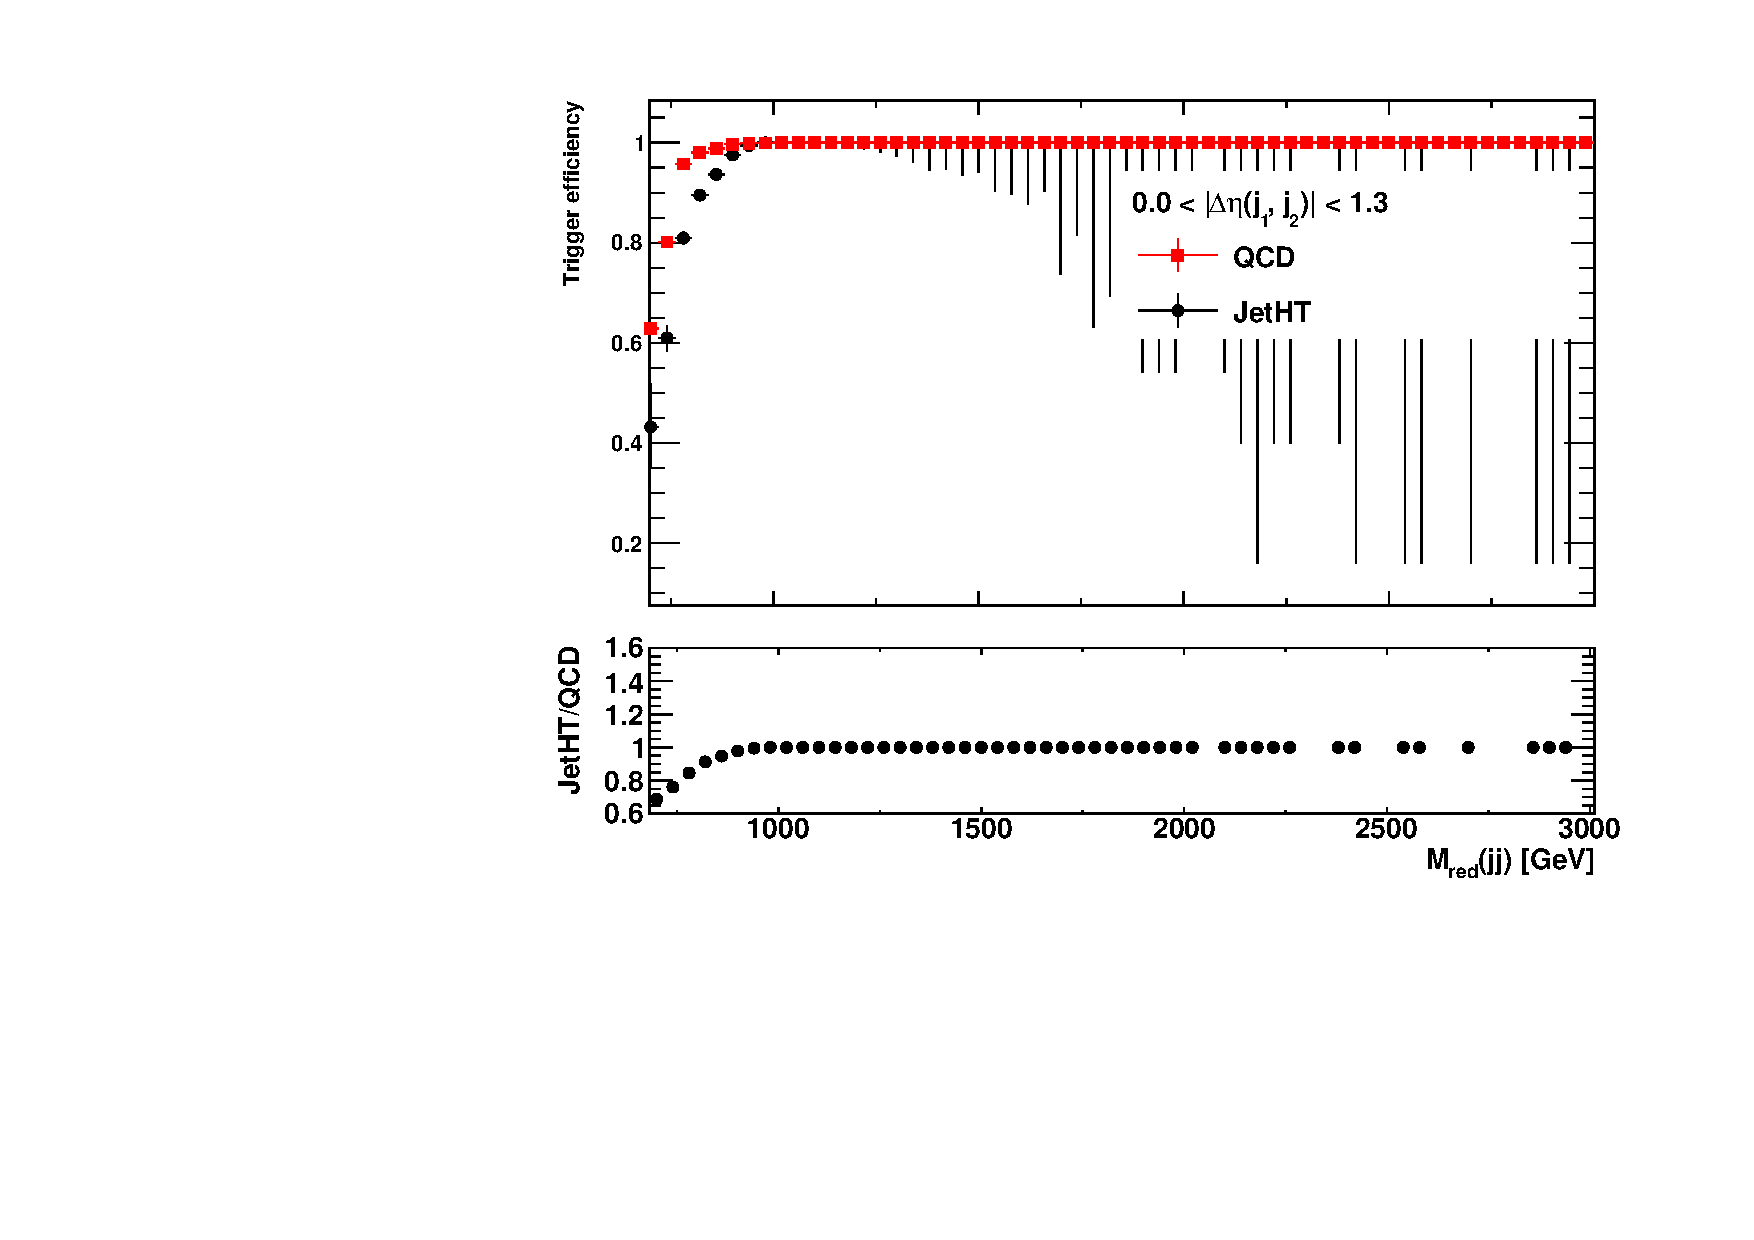
\includegraphics[width=0.45\textwidth]{Analysis/Trigger/JetHT_QCD_mjjred__trigEff.pdf}
    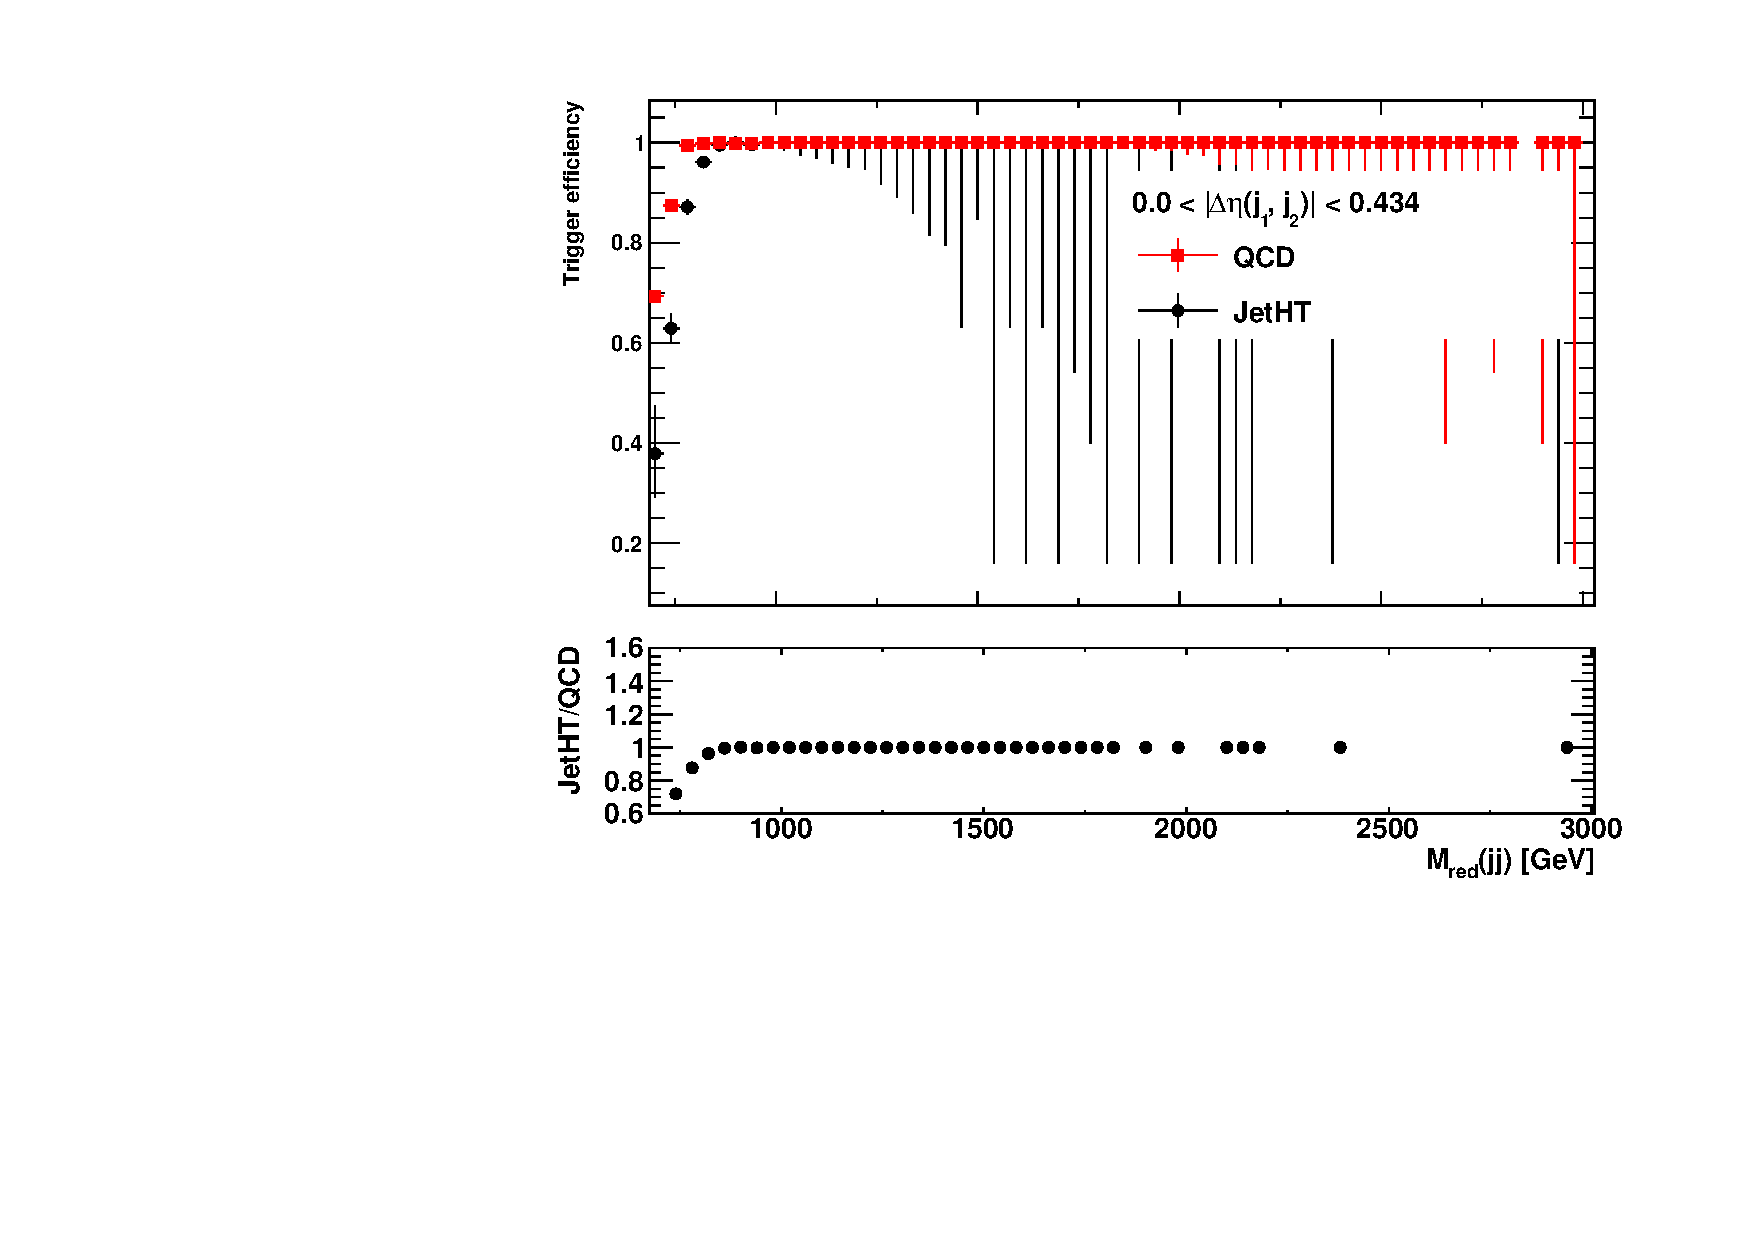
\includegraphics[width=0.45\textwidth]{Analysis/Trigger/JetHT_QCD_mjjred_py0_trigEff.pdf}

    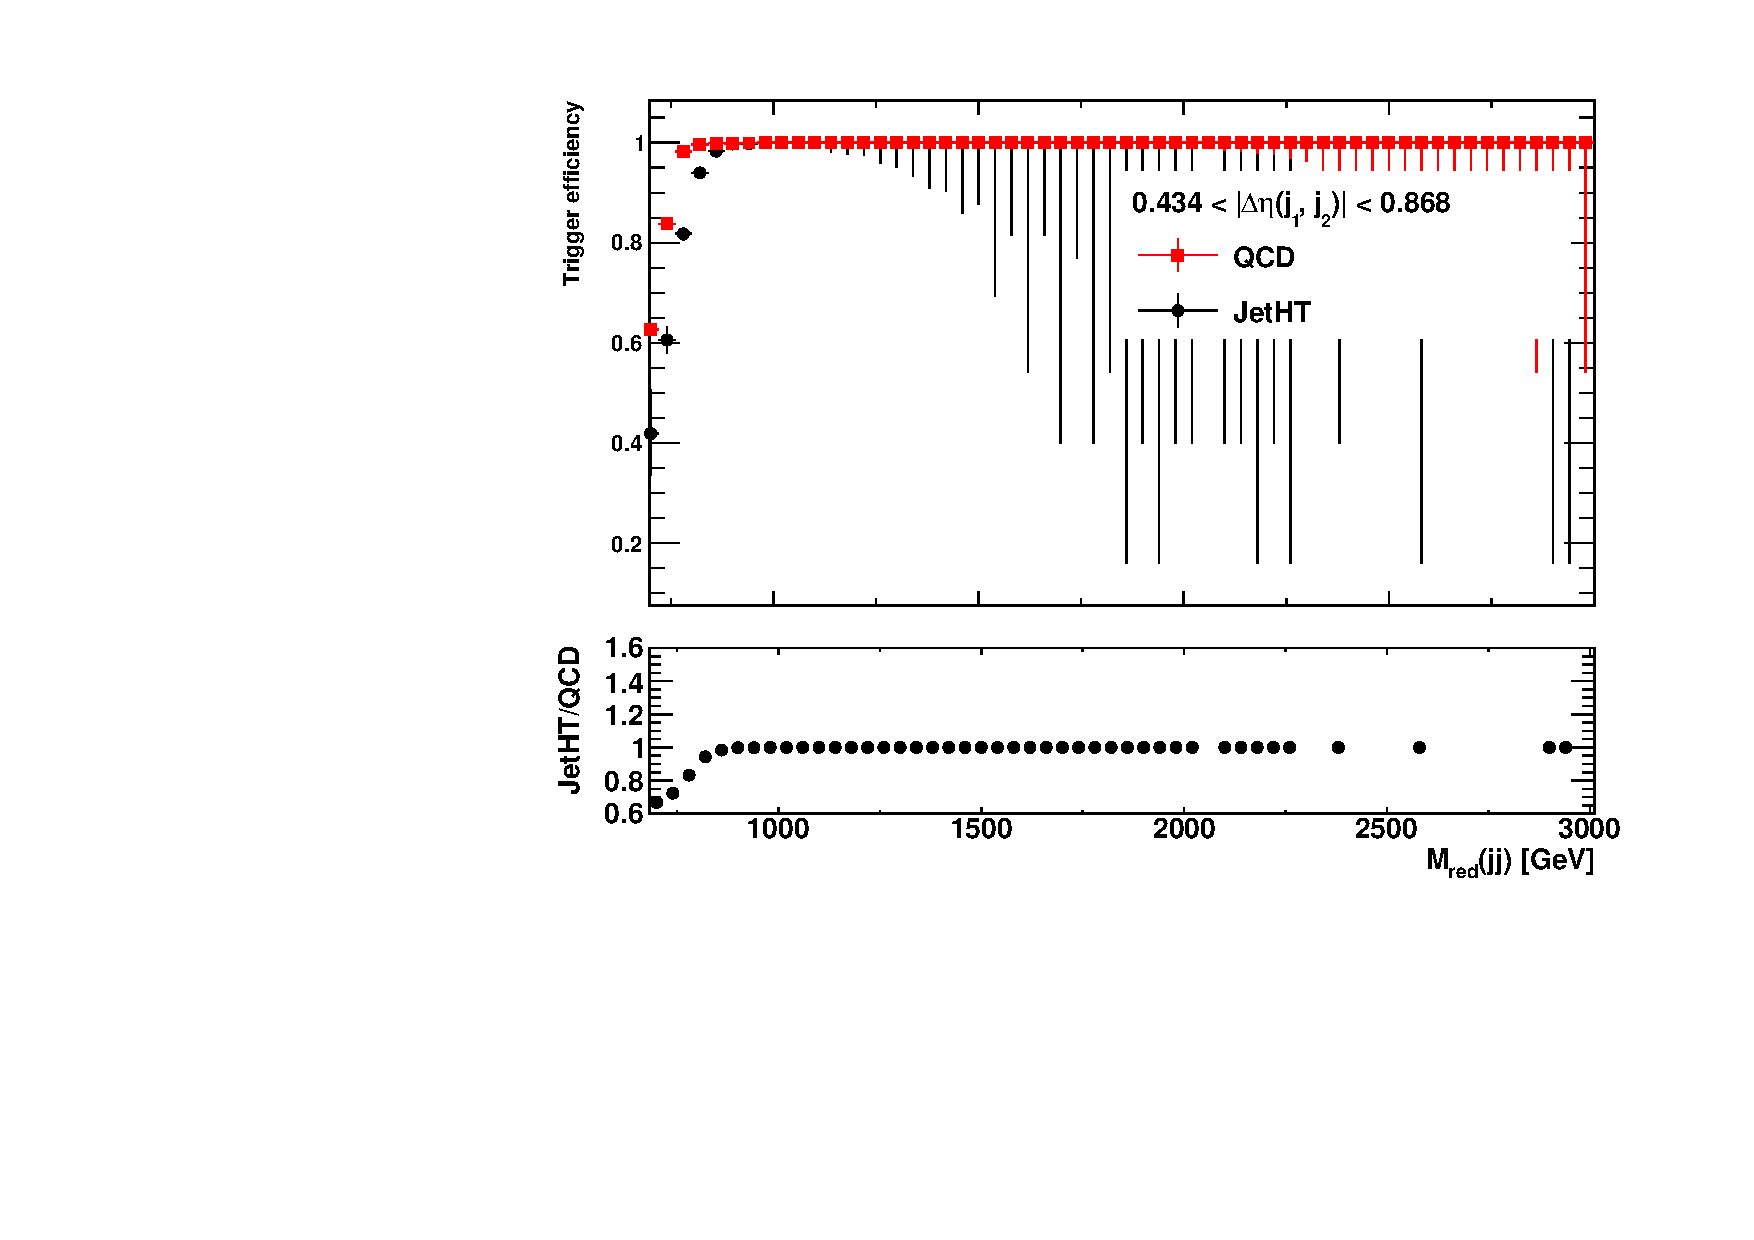
\includegraphics[width=0.45\textwidth]{Analysis/Trigger/JetHT_QCD_mjjred_py1_trigEff.pdf}
    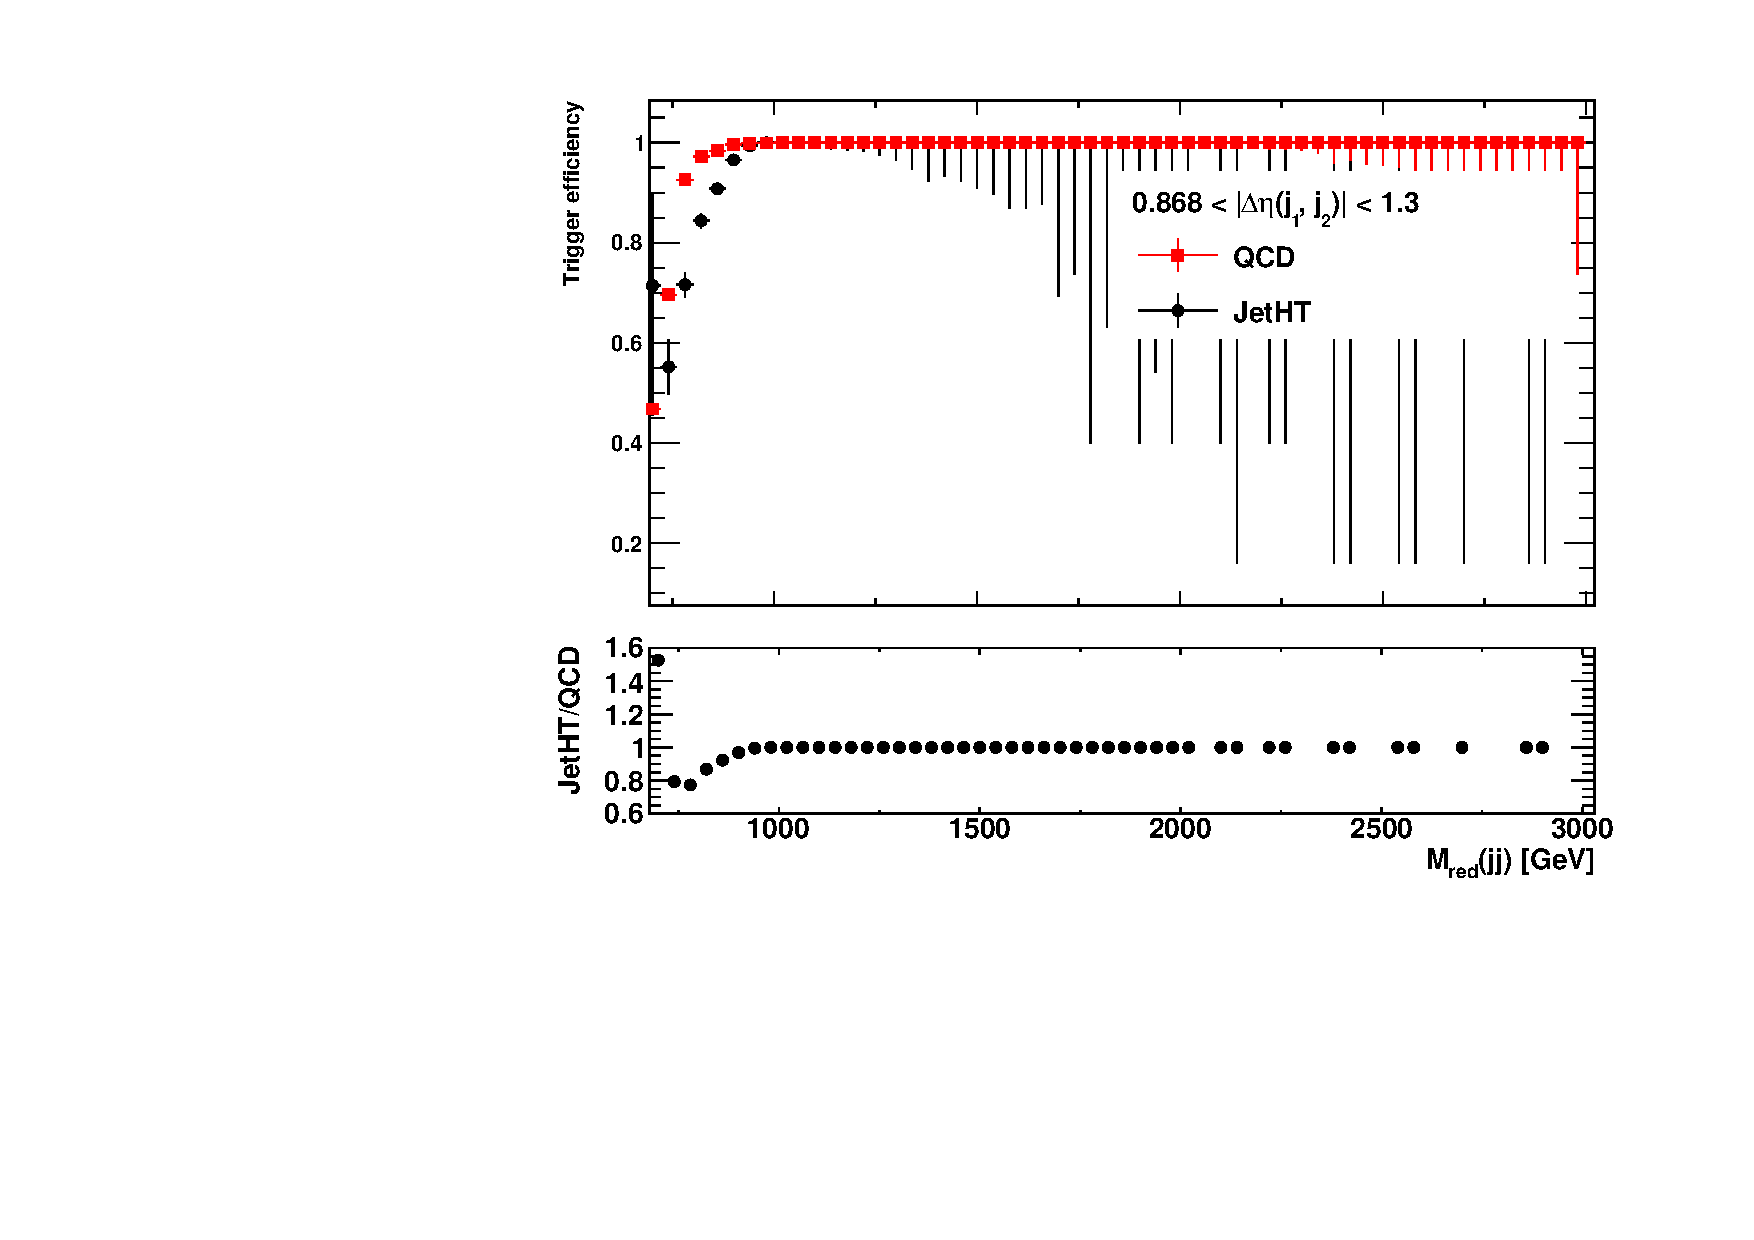
\includegraphics[width=0.45\textwidth]{Analysis/Trigger/JetHT_QCD_mjjred_py2_trigEff.pdf}
  \end{center}
  \caption{The trigger efficiency, as a function of $M_{jj}^{red} \equiv M_{jj} - (M_{jet}^{1}-M_{H}) - (M_{jet}^{2}-M_{H})$, defined in Section~\ref{sss:DijetMassDef}, in the data and QCD MC for different $\Delta\eta_{jj}$ regions: 0.0--1.3 (upper left), 0.0--0.434 (upper right), 0.434--0.868 (lower left), and 0.868--1.3 (lower right).}
  \label{fig:trigeEffvsMjj_JetHT_DetaBins}
\end{figure}

Trigger efficiency is measured as a function of the ``reduced mass'' introduced in Eqn.~\ref{} of Section~\ref{}. The $\Delta\eta_{jj}$ variable is quite different for the signal and the background, and hence the efficiency is measured in three $\Delta\eta_{jj}$ regions: 0.0--0.434, 0.434--0.868, and 0.868--1.3. The efficiencies are shown in Fig.~\ref{fig:trigeEffvsMjj_JetHT_DetaBins}.

\begin{figure}[H]
  \begin{center}
    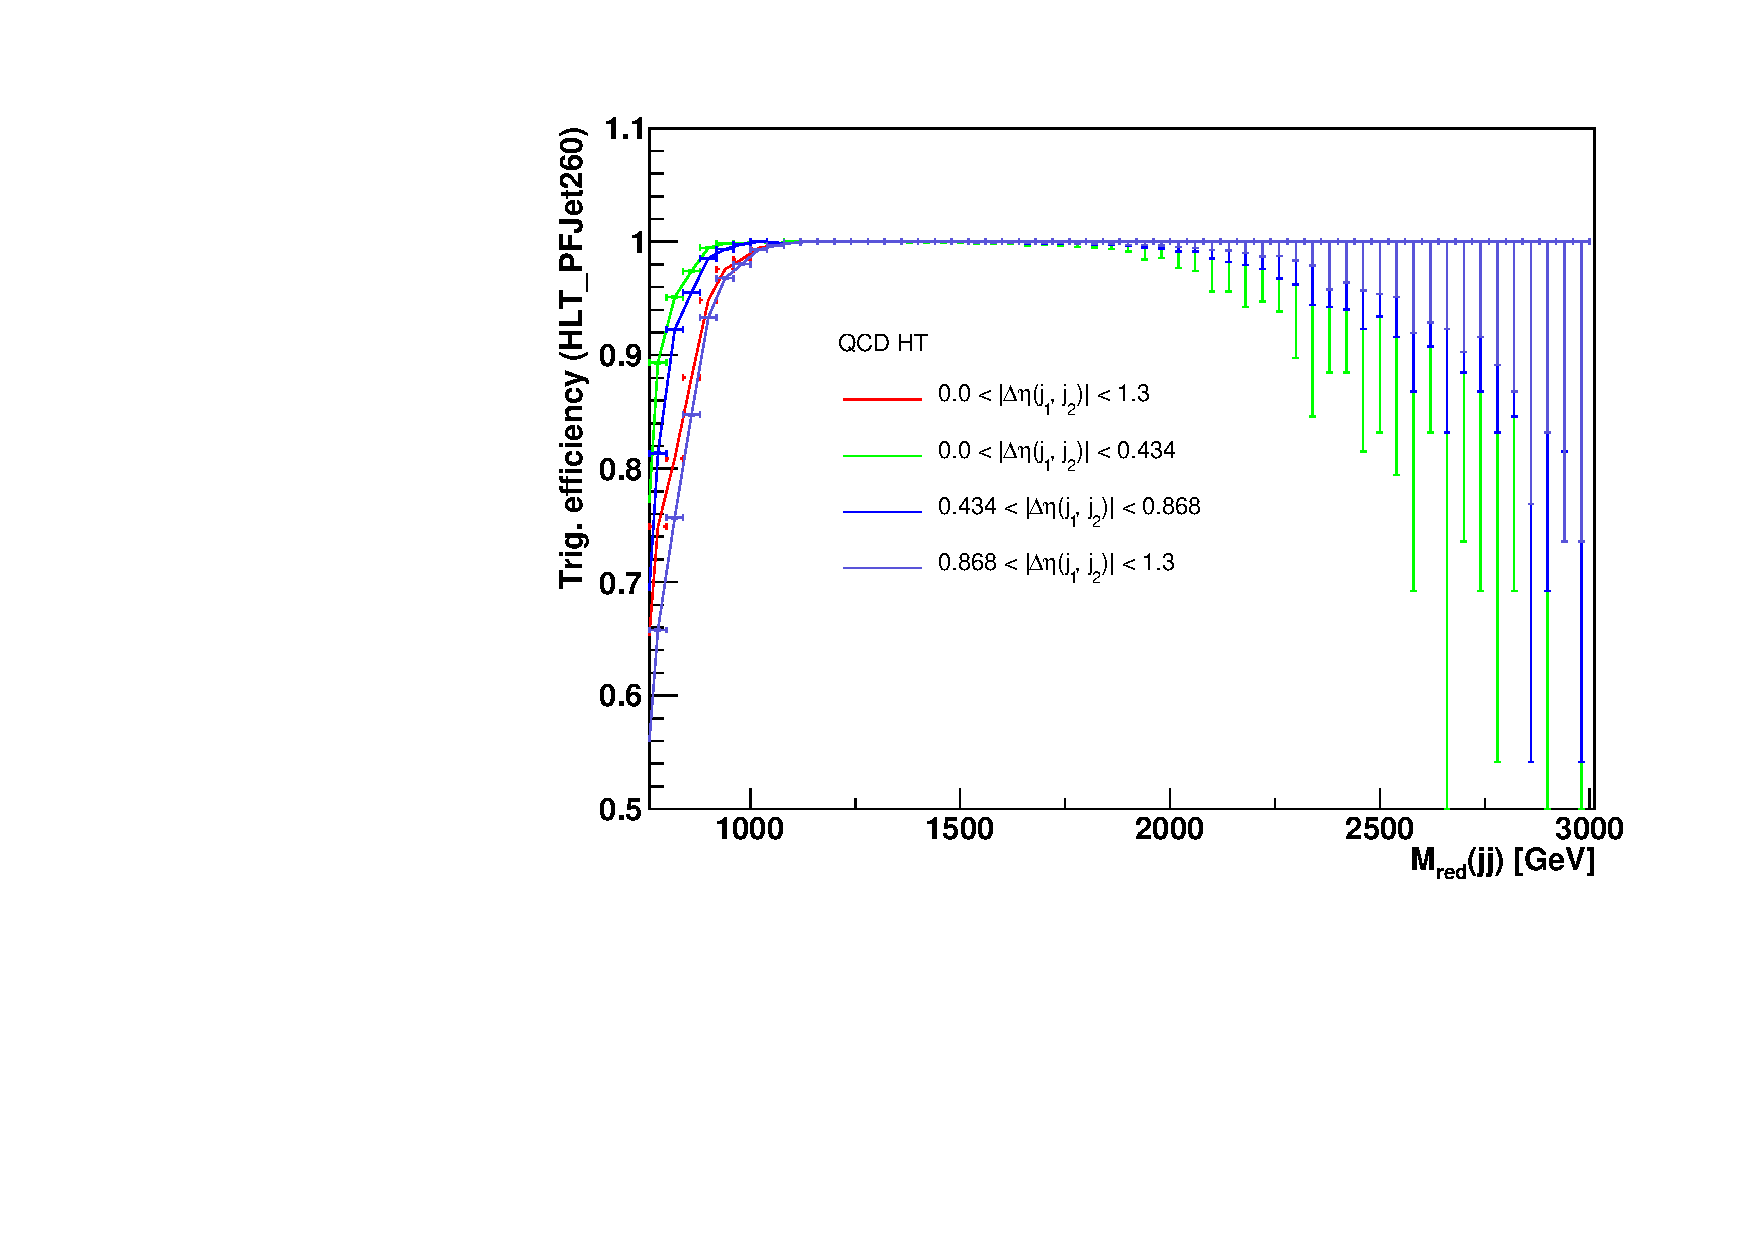
\includegraphics[width=4 in]{Analysis/Trigger/c_QCD_HLTPFJet260.pdf}
  \end{center}
  \caption{The trigger efficiency for the baseline trigger \textsc{HLT\_PFJet260}, as a function of $M_{jj}^{red} \equiv M_{jj} - (M_{jet}^{1}-M_{H}) - (M_{jet}^{2}-M_{H})$, defined in Section~\ref{}, for different $\Delta\eta_{jj}$ regions: 0.0--1.3, 0.0--0.434, 0.434--0.868, and 0.868--1.3. The percentage difference between one and these turn-on curves are taken as an uncertainty on the trigger efficiency scale factor.}
  \label{fig:trigeEffvsMjj_QCDHT_HLTPFJet260_DEtabins}
\end{figure}

The combined set of triggers reaches full efficiciency for $M_{jj}^{red} > 1100$ GeV over all the $\Delta\eta_{jj}$ ranges. For $M_{jj}^{red} < 1100$ GeV, the trigger efficiencies are higher for smaller $\Delta\eta_{jj}$, where most of the signal lie, and are smaller at larger values of $\Delta\eta_{jj}$. Furthermore, the data/MC scale factor also varies depending on $\Delta\eta_{jj}$. Since the search begins from $M_{jj}^{red} = 750$ GeV, the modelling of the trigger efficiency turn-on curves in the data and the simulations are done extremely carefully. Since the baseline trigger \textsc{HLT\_PFJet260} also has some inefficiency for low $M_{jj}^{red}$, an additional uncertainty is assigned to the trigger efficiency scale factor based on this trigger's efficiency  in MC.

Figure~\ref{fig:trigeEffvsMjj_QCDHT_HLTPFJet260_DEtabins} shows the \textsc{HLT\_PFJet260} trigger turn-on curves for different $\Delta\eta_{jj}$ in MC, with respect to only the event selection. The difference between unity and the trigger efficiency is propagated to the scale factor as a systematic uncertainty. The scale factors are shown in Fig.~\ref{fig:trigeEffSFvsMjj_JetHT_DetaBins}. The trigger efficiency is also measured in different run periods separately. The efficiency turn-on curves are shown in Fig.~\ref{fig:Mjj_trigeEffvsMjj_JetHT}.

\begin{figure}[H]
  \begin{center}
    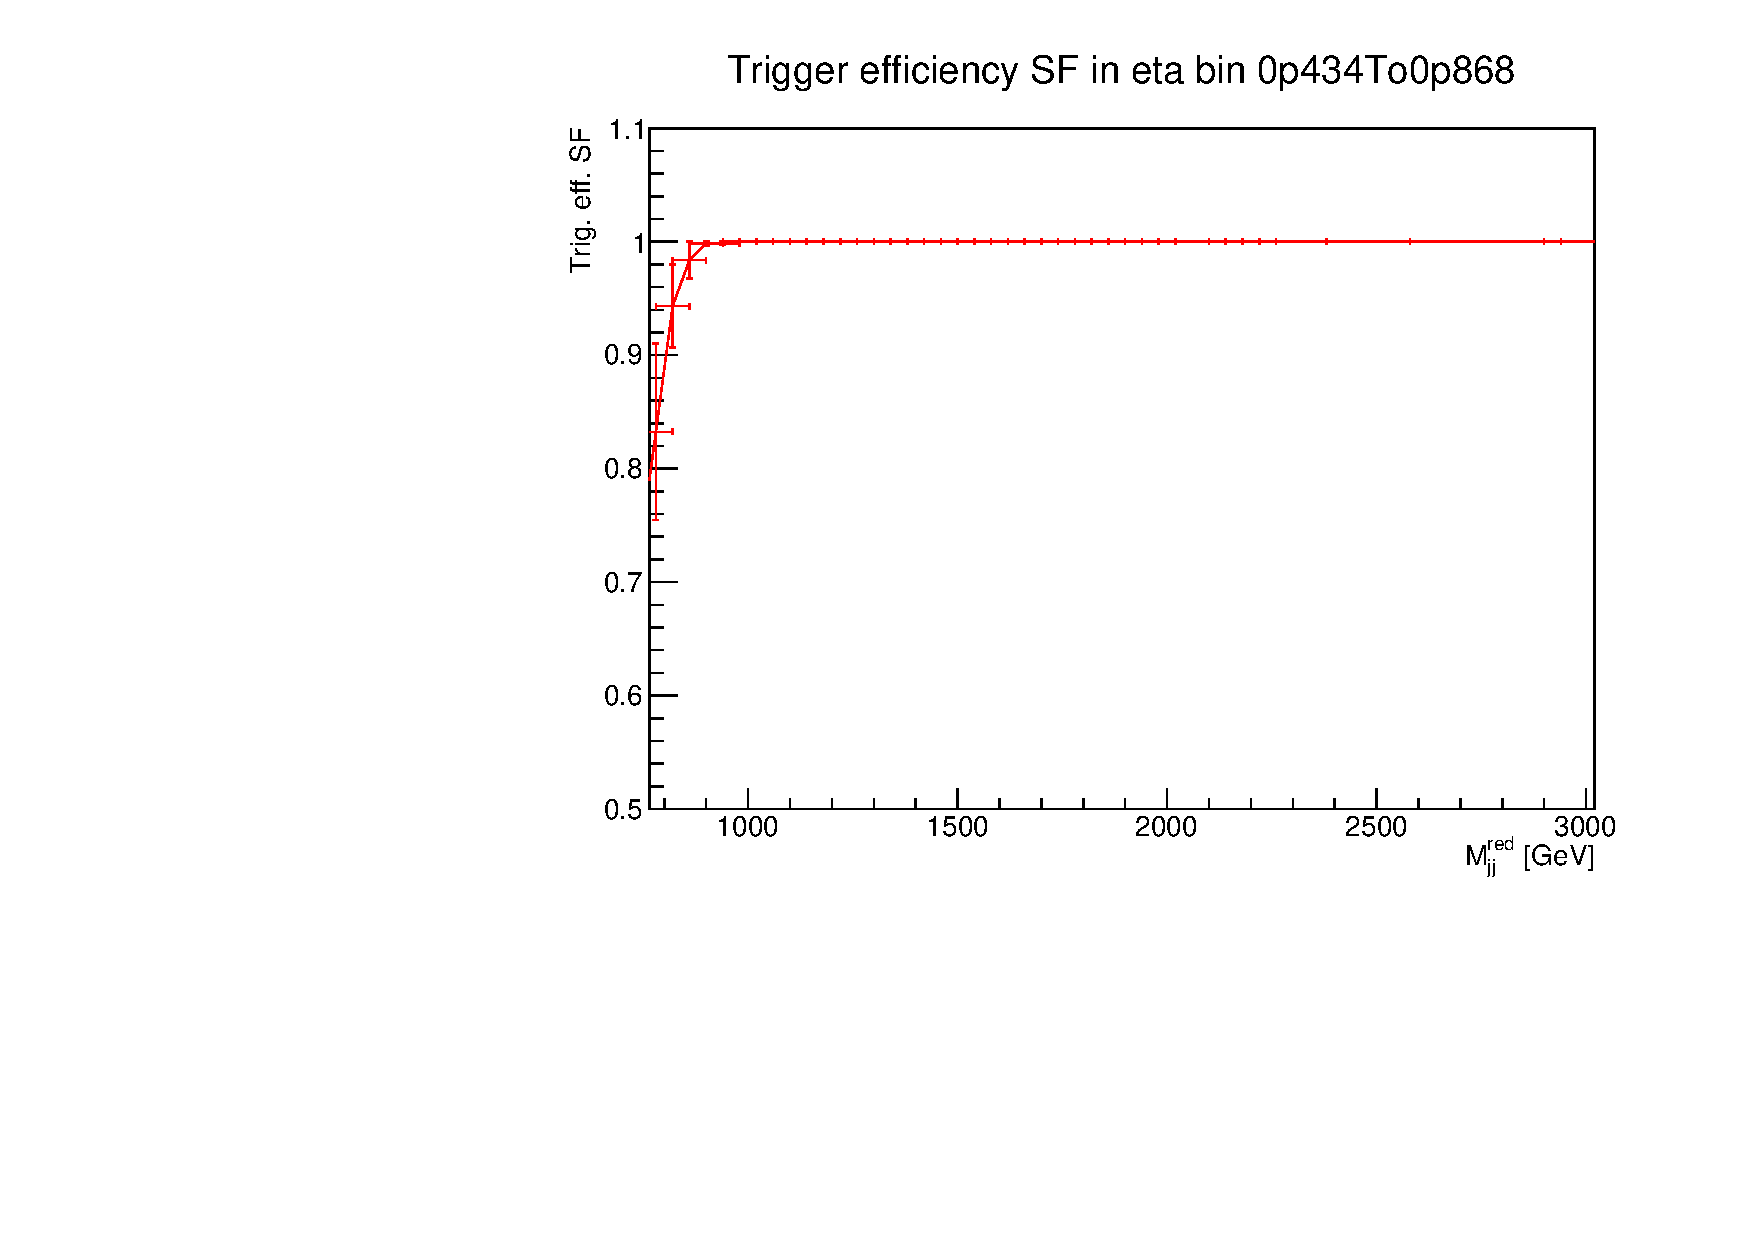
\includegraphics[width=0.33\textwidth]{Analysis/Trigger/c_gsftrigger_0p434To0p868}
    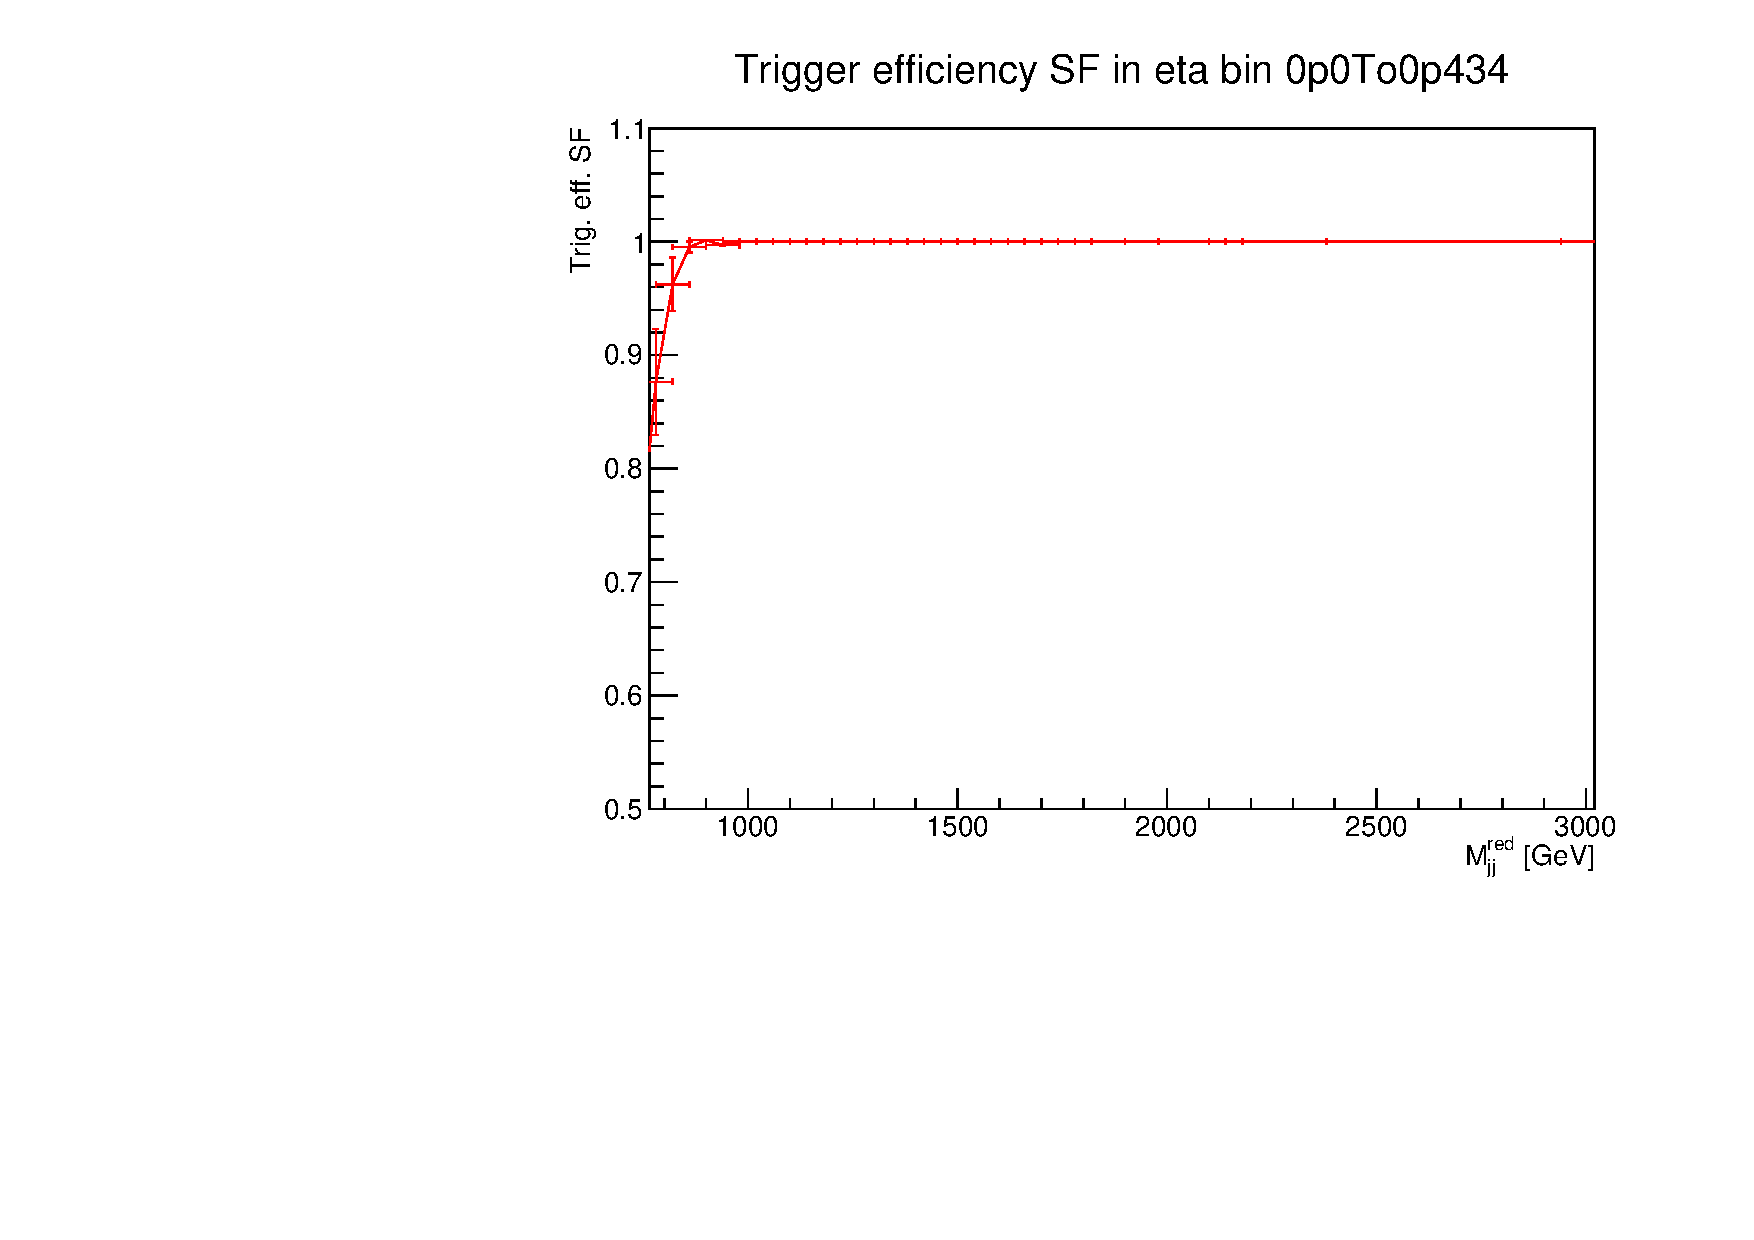
\includegraphics[width=0.33\textwidth]{Analysis/Trigger/c_gsftrigger_0p0To0p434}
    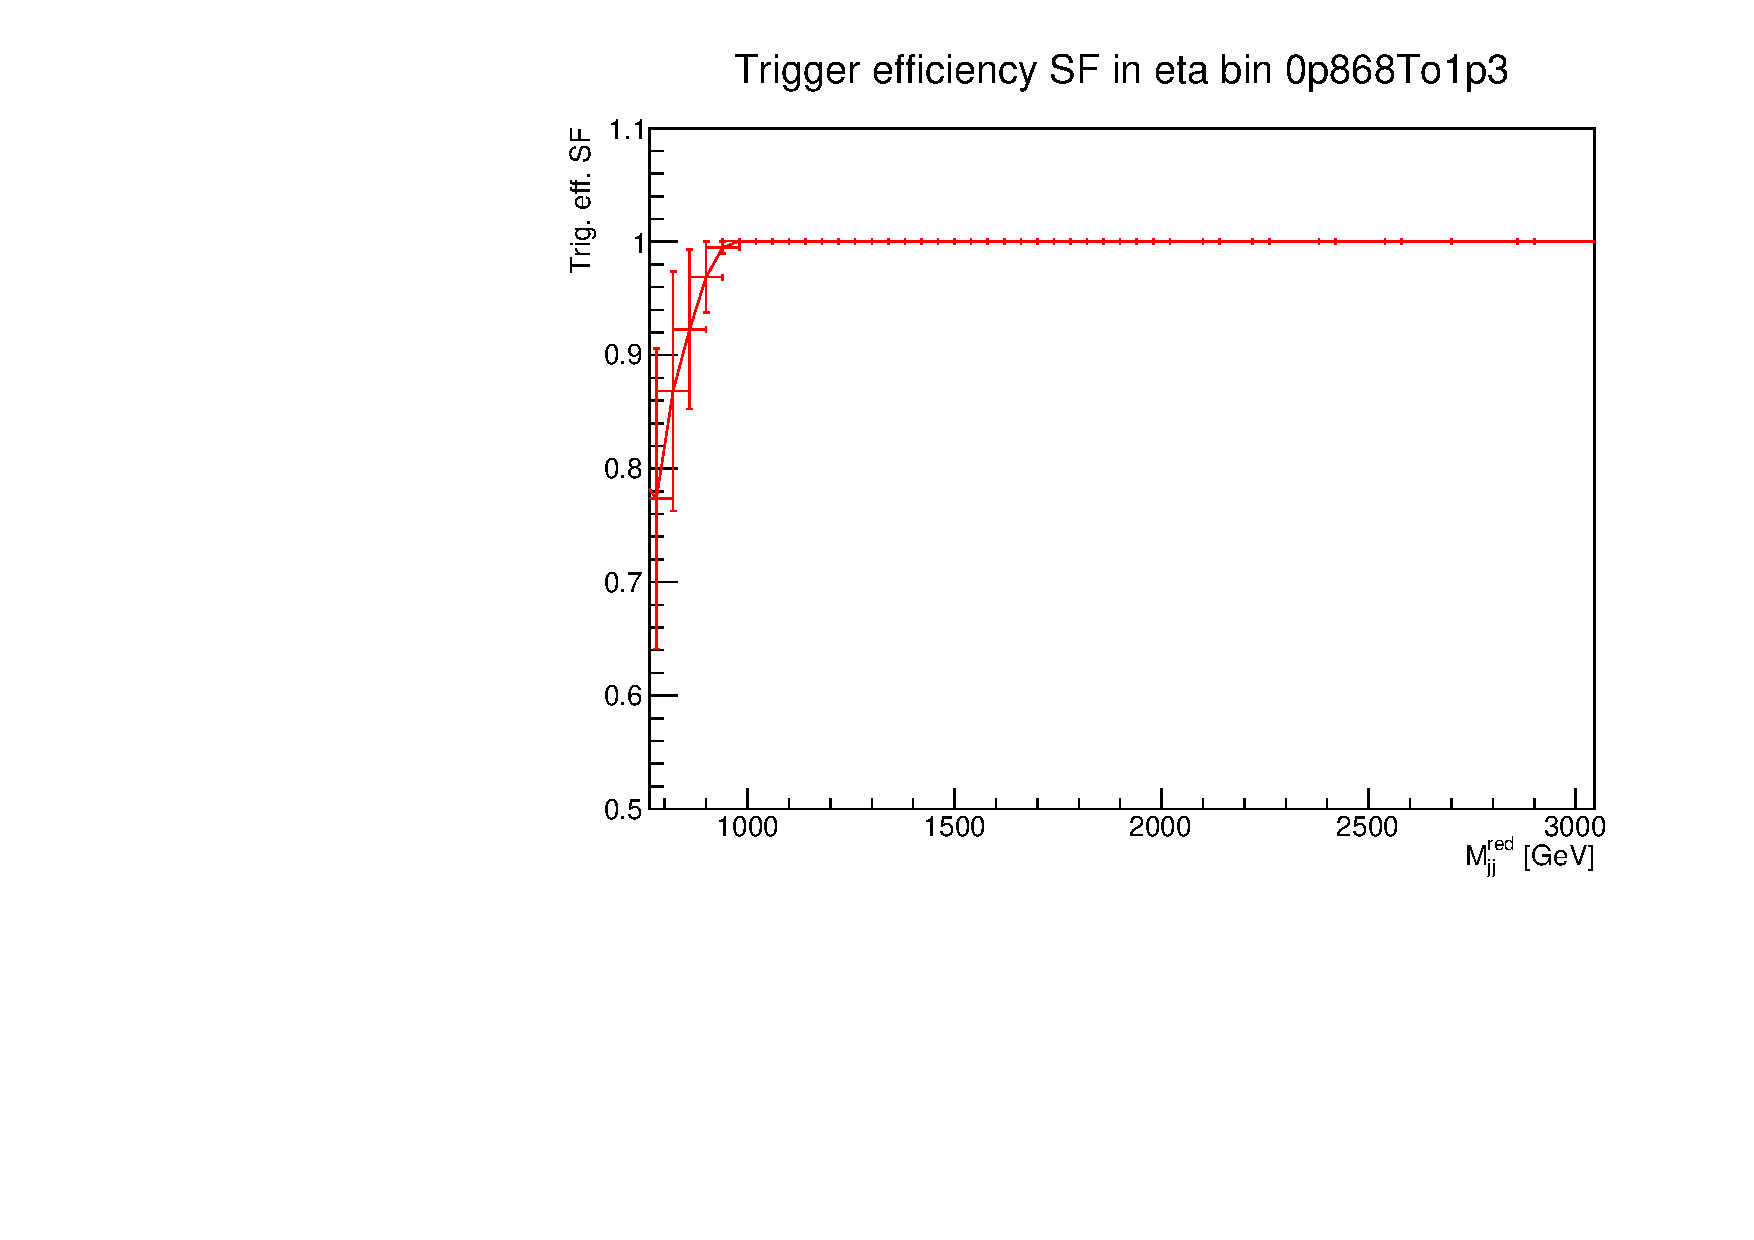
\includegraphics[width=0.33\textwidth]{Analysis/Trigger/c_gsftrigger_0p868To1p3}
  \end{center}
  \caption{The trigger efficiency scale factors, as a function of $M_{jj}^{red} \equiv M_{jj} - (M_{jet}^{1}-M_{H}) - (M_{jet}^{2}-M_{H})$, defined in Section~\ref{}, for different $\Delta\eta_{jj}$ regions: 0.0--0.434 (left), 0.434--0.868 (centre), and 0.868--1.3 (right). The error bars are the combined statistical and systematic errors.}
  \label{fig:trigeEffSFvsMjj_JetHT_DetaBins}
\end{figure}


\begin{figure}[H]
  \begin{center}
    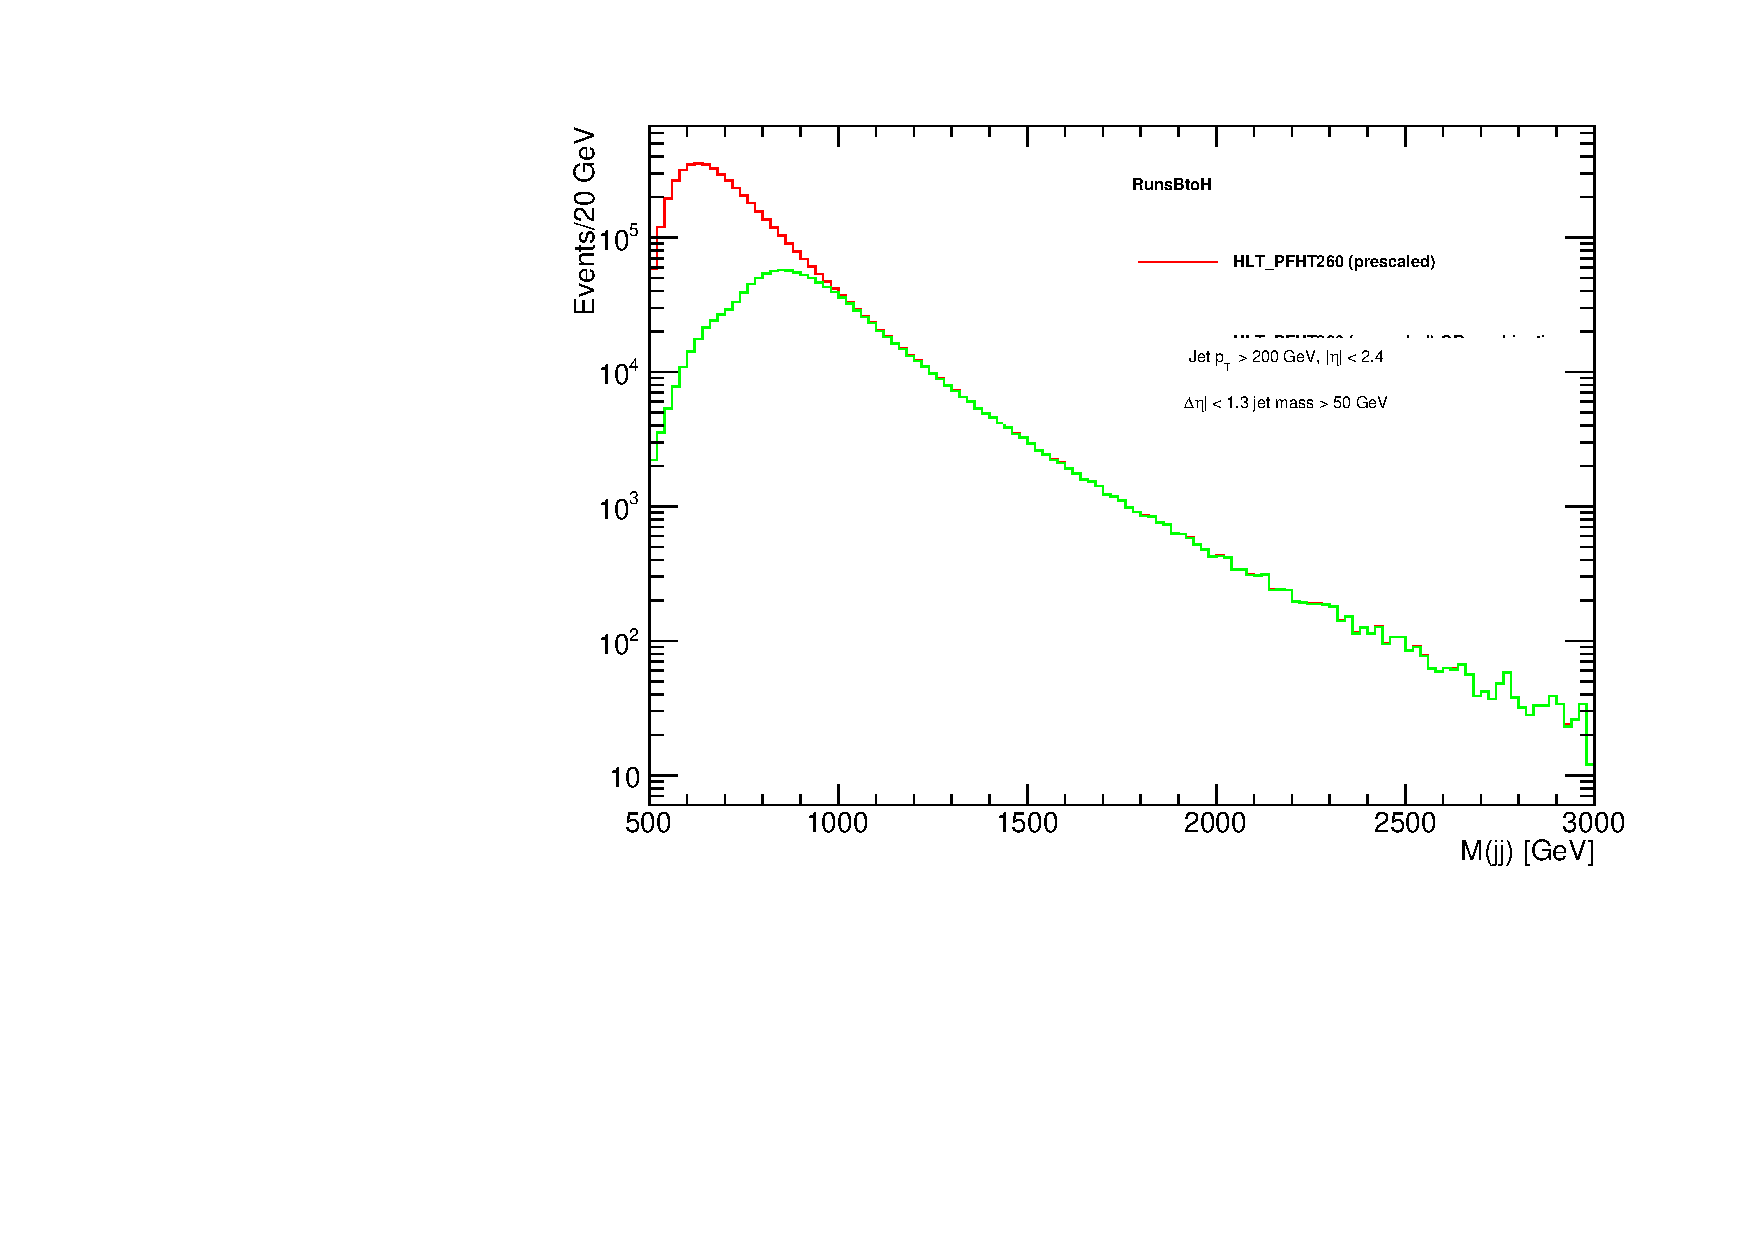
\includegraphics[scale=0.32]{Analysis/Trigger/JetHT_RunsBtoH_mjj_all_pass.pdf}
    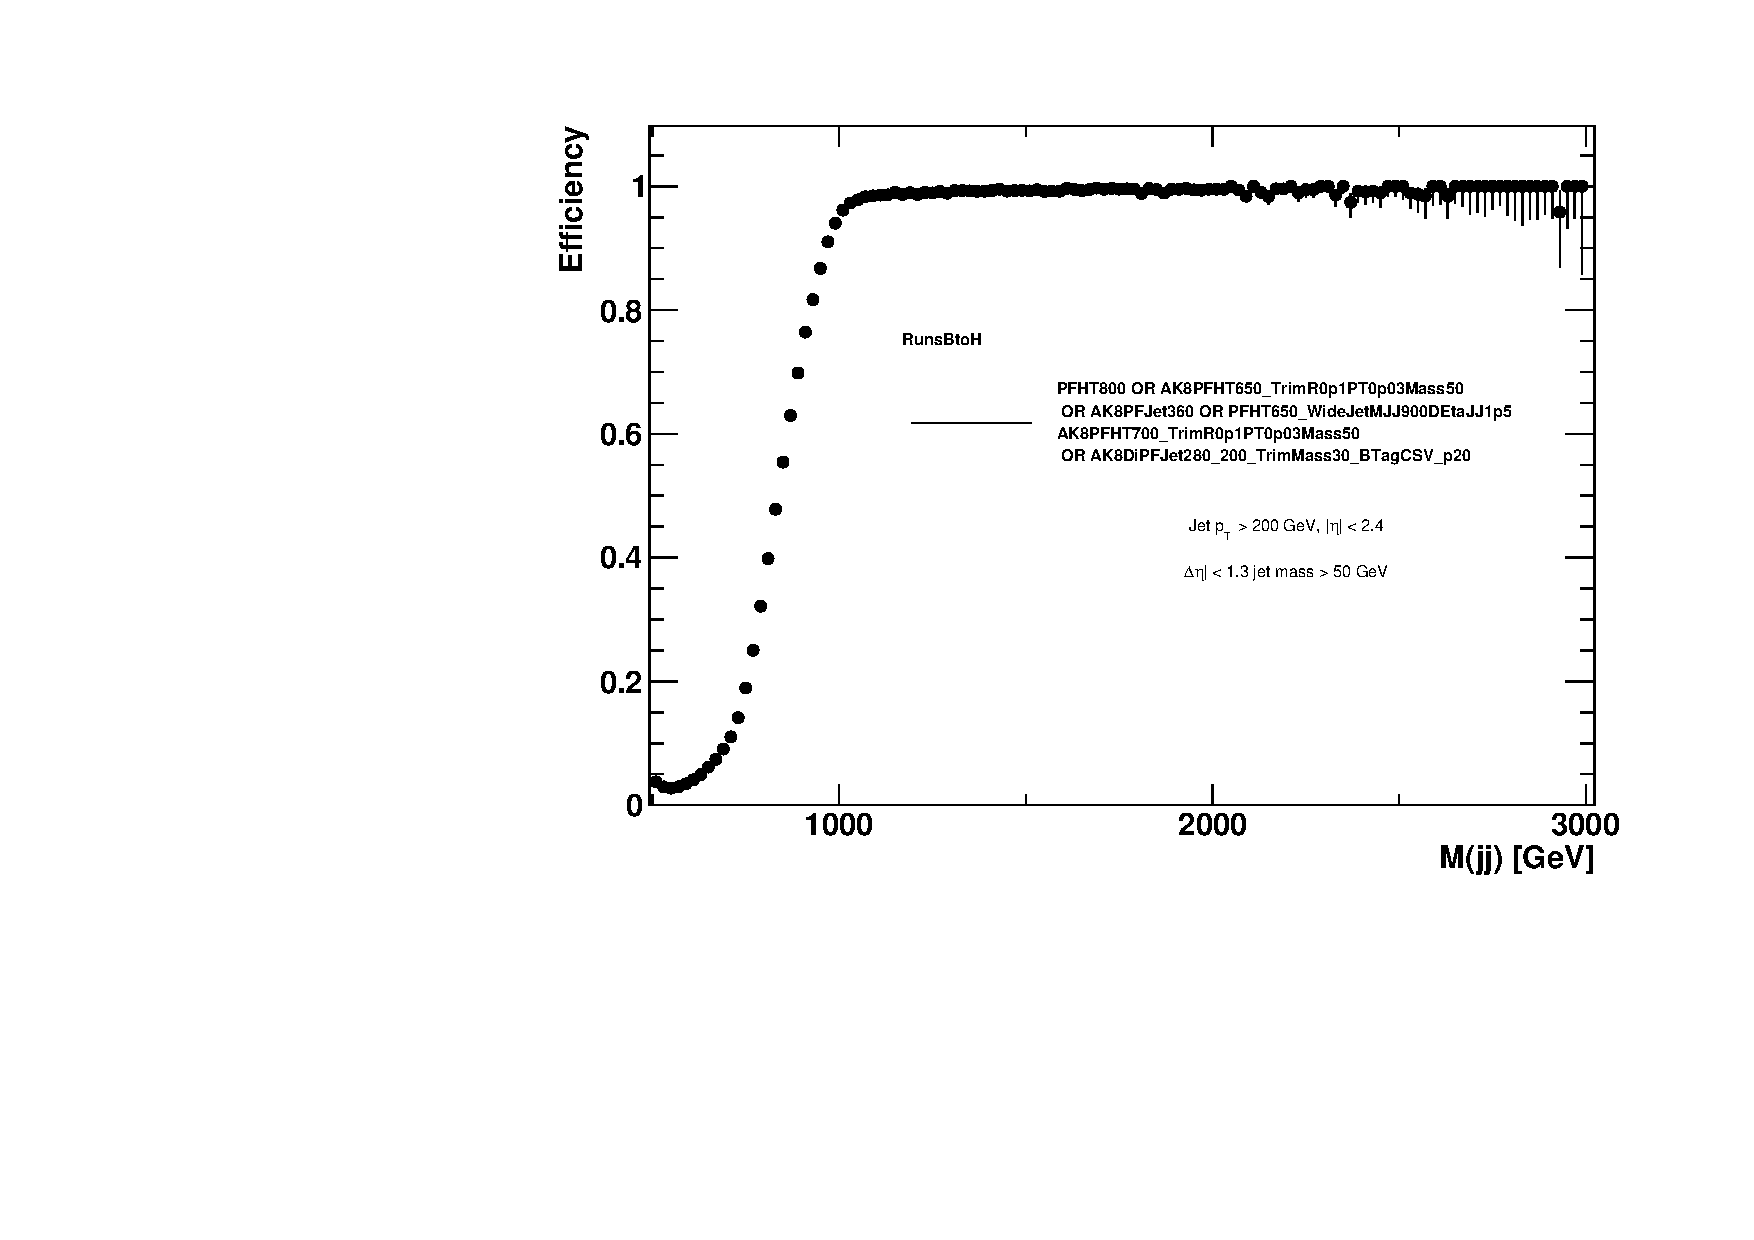
\includegraphics[scale=0.32]{Analysis/Trigger/JetHT_RunsBtoH_trigeff_mjj.pdf}
    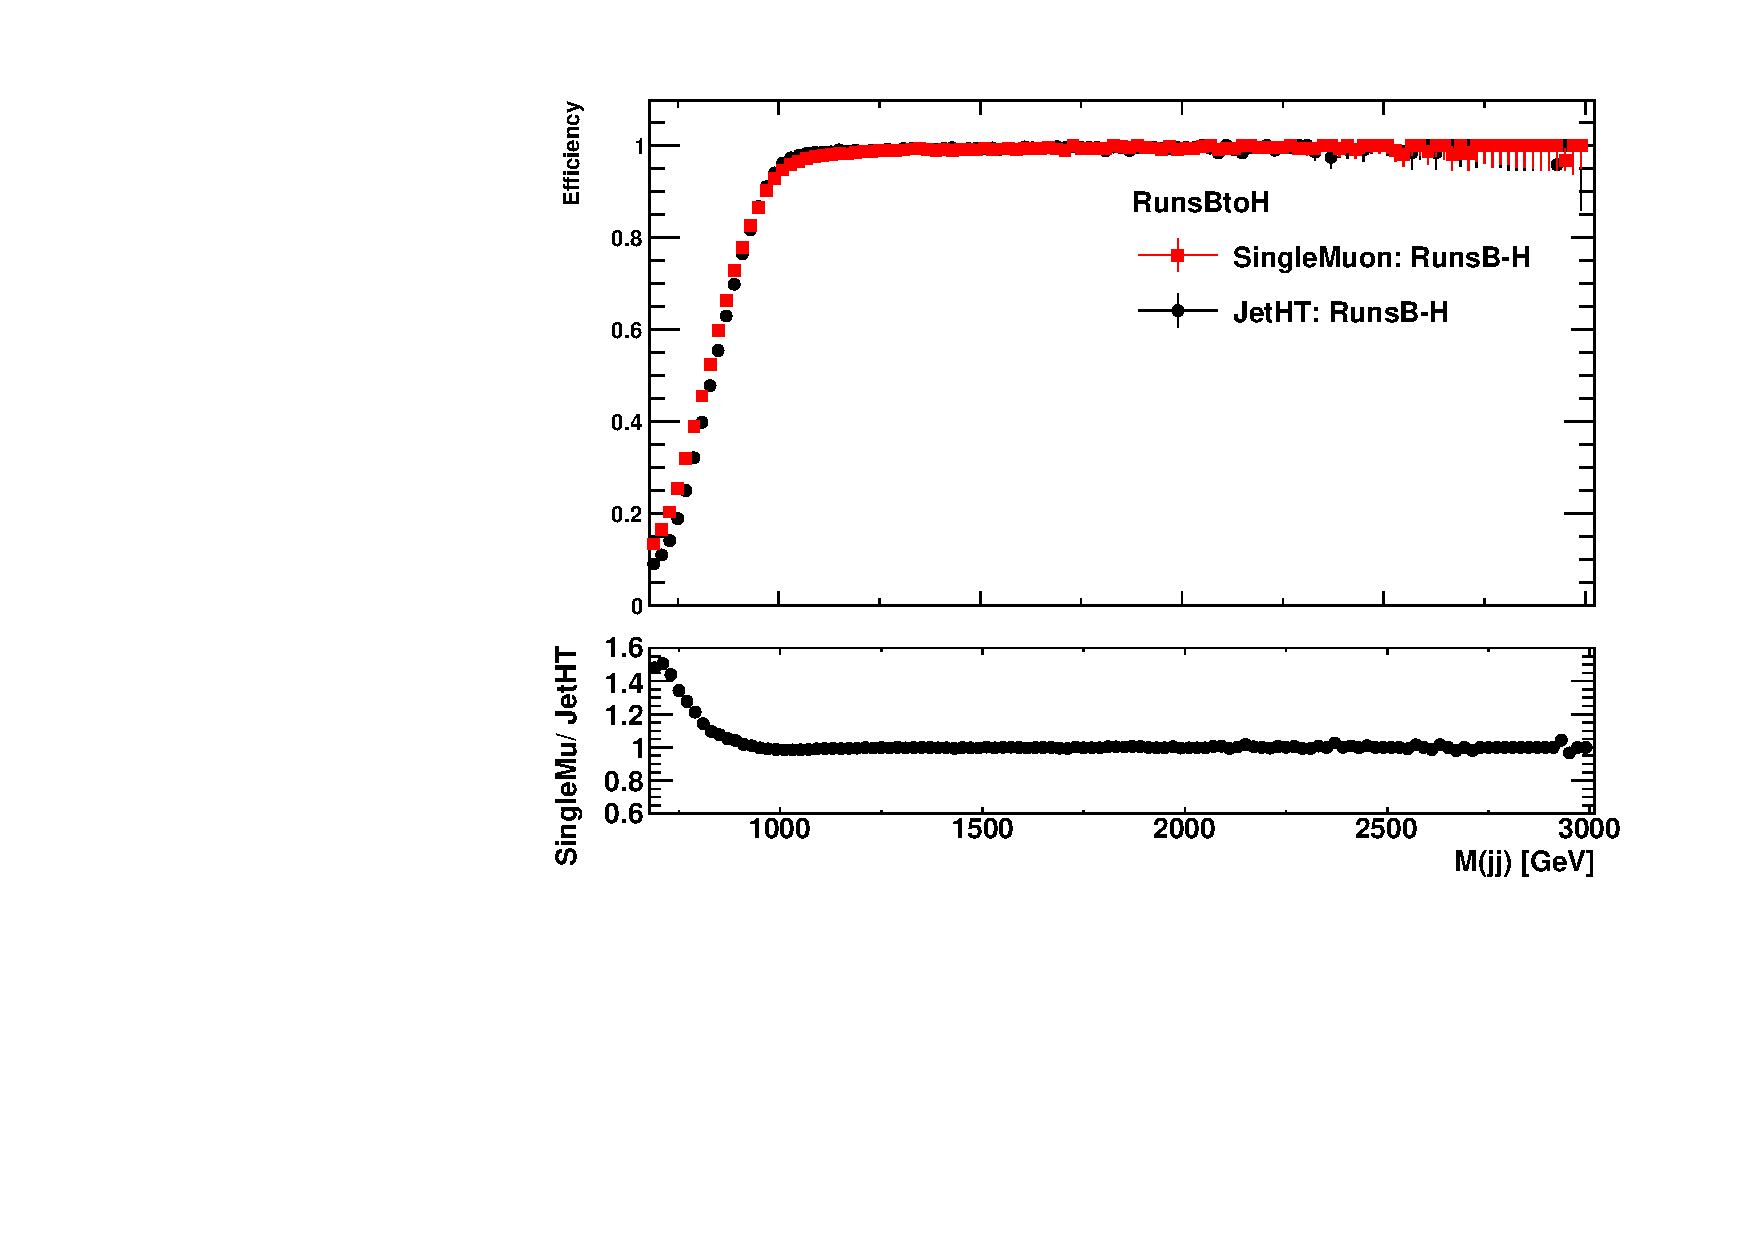
\includegraphics[scale=0.32]{Analysis/Trigger/JetHT_SingleMuon_BtoH_mjj_trigEff.pdf}
  \end{center}
  \caption{The dijet mass distribution used to derive the efficiency in data (top left) and the trigger efficiency as measured in data (top right) using the \texttt{JetHT} dataset. The bottom figure shows the ratio of the turn-on curves from the \texttt{SingleMuon} over the \texttt{JetHT} datasets.}
  \label{fig:Mjj_trigeEffvsMjj_JetHT}
\end{figure}

\section{Event Selection}
\label{sec:EvtSel}

After passing the triggers, events are required to have at least one reconstructed $pp$ collision vertex satisfying the following criteria:
\begin{itemize}
  \item Vertex number of degrees of freedom $> 4$;
  \item Absolute displacement from the beamspot position along the $z$ direction $< 24$ cm;
  \item Absolute displacement from the beamspot position along the transverse direction $< 2$ cm.
\end{itemize}

\noindent
Many additional vertices, corresponding to other overlapping $pp$ collisions (pileup), are usually reconstructed in an event using charged particle tracks. The primary interaction vertex (PV) corresponds to the vertex that maximizes the sum in $p_{T}^2$ and the magnitude of $\sum{p_{T}}$ from the associated physics objects.

\subsection{Lepton Selection}

To suppress $\mathrm{t\bar{t}} + \mathrm{jets}$ and diboson backgrounds, events with an isolated electron or muon with $p_{T} > 20$ GeV are removed. The isolation requirement is designed to remove jets misidentified as leptons and is defined as the ratio of energy surrounding the lepton and the leptons momentum. The energy surrounding a lepton is defined as the scalar $p_{T}$ sum of the charged hadrons, neutral hadrons, and photons in a cone of $\Delta R = 0.3$ and $\Delta R = 0.4$ for electrons and muons, respectively. The identification criteria for an electron and a muon a listed in Tables~\ref{tab:electronid} and~\ref{tab:muonid}, respectively. The combined isolation and identification requirement of the lepton is required to be such that the overall electron selection efficiency is $90\%$ ($70\%$) for the "loose" ("medium") requirement. For the "loose" ("medium") muons, the selection efficiency is $100\%$ ($95\%$). Events are rejected if they contain one lepton passing the medium requirement or two leptons passing the loose requirement that have the same flavor but opposite charge.

\begin{table}[htb]
  \begin{center}
    \begin{tabular}{l |l | l | l | l}
    \hline
    \hline
       & \multicolumn{2}{c}{Barrel Selection} &
    \multicolumn{2}{| c}{Endcap Selection}\\
    \hline
    Variable & Loose &  Medium & Loose & Medium\\
    \hline
    $5\times 5 \sigma_{i\eta i\eta} < $ & 0.011 & 0.00998 & 0.0314 & 0.0298  \\
    $\Delta \eta_{seed} < $ & 0.00477 & 0.00311 & 0.00868 & 0.00609  \\
    $\Delta \phi_{in} <$  & 0.222 & 0.103 & 0.213 & 0.045     \\
    H/E $<$   & 0.298 & 0.253 & 0.101 & 0.0878   \\
    $|\frac{1}{E} - \frac{1}{p}| <$ & 0.241 & 0.134 & 0.14 & 0.13   \\
    Missing hits $\leq$   & 1 & 1 & 1 & 1     \\
    Conversion veto     & yes & yes & yes & yes \\
    \hline
    \hline
    \end{tabular}
   \caption{Loose and medium electron identification criteria used in the analysis.The selection criteria varies depending on if the electron is in the barrel or endcap of the detector. \label{tab:electronid}}
  \end{center}
\end{table}

\begin{table}[htb]
  \begin{center}
    \begin{tabular}{l | l}
    \hline
    \hline
    Loose &  Medium \\
    \hline
    Global or Tracker Muon     & Global Muon  \\
    PF Muon  & Normalized $\chi^{2}$ of the global track $< 3$     \\
      & Tracker-Standalone position match $< 12$  \\
      & Kink finder $< 20$     \\
      & segment compatibility $> 0.303$      \\
      & OR \\
      & segment compatibility $> 0.451$ \\
    \hline
    \hline
    \end{tabular}
   \caption{Loose and medium muon identification criteria used in the analysis. A segment is when hits in the muon drift tubes and cathode strip chambers are matched.\label{tab:muonid}}
  \end{center}
\end{table}

\subsection{Jet Selection}

Particle Flow (PF) candidates, as described in Section~\ref{}, are clustered using the anti-$k_{t}$ algorithm~\cite{antikt}, as described in Section~\ref{}, implemented in \textsc{FastJet}~\cite{FastJet}, into jets with a distance parameter $R=0.8$ (referred to as AK8 jets). To mitigate the effecrt of pileup, particles are assigned weights using the pileup per particle identification (PUPPI) algorithm~\cite{PUPPI}. This method uses local shape information, event pileup properties, and tracking information to compute a weight describing the degree to which a particle is pileup-like. Charged particles from pileup vertices recieve a weight of zero while those from the primary vertex receive a weight of one. Neutral particles are assigned a weight between zero and one, with higher values for those likely to originate from the primary vertex.

To account for detector response nonlinearity, jet energy corrections (JECs) are applied as a function of jet $\eta$ and $p_{T}$~\cite{JEC, JEC2}. The JECs applied to both data and MC are known as L2L3 MC-truth corrections. This correction is derived from simulation and is designed to make the jet response uniform in $\eta$ and $p_{T}$. An additional L2L3 residual correction is applied to data events to correct for the small differences within jet response in data and MC. The procedure for the uncertainties associated with these corrections is described in Section~\ref{}. 

In each event, the $h\rightarrow \mathrm{b\bar{b}}$ system is reconstructed as a single high-$p_{T}$ AK8 jet, where the decay products have merged within the jet, and the two highest $p_{T}$ jets in the event are assumed to be the Higgs boson candidates. Both Higgs boson candidates are required to have $p_{T} > 300$ GeV and $|\eta| < 2.4$. All jets are also required to pass the tight jet identification requirements provided by the CMS JetMET physics analysis group. These selections require a jet to have a neutral hadron fraction $< 0.9$, a neutral EM fraction $< 0.9$, a muon fraction $< 0.8$, a charged hadron fraction $> 0$, a charged EM fraction $< 0.9$, and more than 1 constituent. The hadron fraction is the percentage of jet constituents taken from HCAL hits, the EM fraction is the percentage of jet constituents taken from ECAL hits, and the muon fraction is the percentage of constituents taken from the muon detector. All of these requirements are summarized in Table~\ref{tab:tightjetid}.

\begin{table}[htb]
  \begin{center}
    \begin{tabular}{l r}
    \hline
    \hline
    Variable &  Cut \\
    \hline
    Neutral Hadron Fraction & $<0.90$  \\
    Neutral EM Fraction     & $<0.90$  \\
    Number of Constituents  & $>1$     \\
    Muon Fraction           & $<0.8$   \\
    Charged Hadron Fraction & $>0$     \\
    Charged Multiplicity    & $>0$     \\
    Charged EM Fraction     & $< 0.90$ \\
    \hline
    \hline
    \end{tabular}
   \caption{Tight jet identification quality criteria used in the analysis.\label{tab:tightjetid}}
  \end{center}
\end{table}

For multijet background events, the two AK8 jets have a large separation in $\eta$. In contrast, the signal events are characterized by a small separation of the two jets. Therefore, events are required to have a pseudorapidity separation $|\Delta\eta(\mathrm{j}_{1}, \mathrm{j}_{2})| < 1.3$. 

\begin{figure}[htbp]
\begin{center}
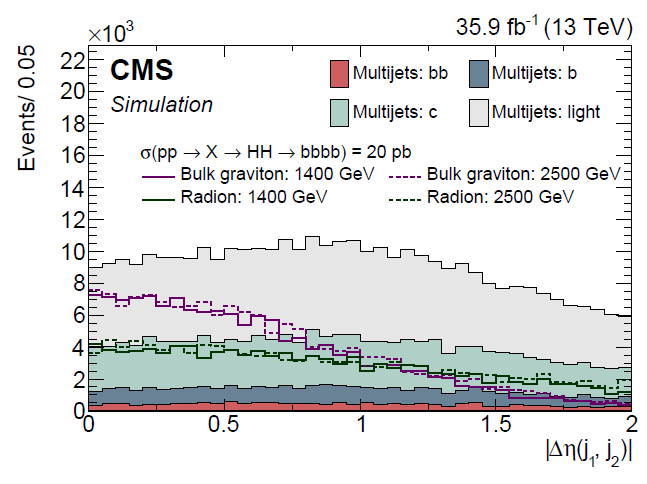
\includegraphics[width=4 in]{Analysis/EventSelection/DeltaEta.png}
\end{center}
\caption{The jet separation, $|\Delta\eta(\mathrm{j}_{1}, \mathrm{j}_{2})|$, distribution for background and signal events. The multijet background components for the differernt jet flavors are shown: events containing at least one jet with two B hadrons (bb) or a single one (b), events containing a jet having a charm hadron (c), and all other events (light). Also, the simulated bulk graviton and radion signals of masses 1400 and 2500 GeV.}
\label{fig:DeltaEta}
\end{figure}

\subsubsection{Candidate Higgs Selection}

After the initial preselction, further cuts need to be applied to reduce the large amount of QCD background. These cuts all have the same effect of distinguishing a standard QCD jet from a Higgs jet. First, a selection is applied to the mass of each jet. The jet is first groomed~\cite{JetGrooming} to mitigate the effects of initial state radiation, underlying event activity, and pileup. This done with the soft-drop algorithm~\cite{SDMass, SDMass2} which is a declustering algorithm that recursively removes soft wide-angle radiation from a jet. The soft-drop declustering procedure begins by undoing the last step of the jet clustering by breaking the jet, $j$, into two subjets, $j_{1}$ and $j_{2}$. If the subjets pass the soft-drop condition:

\begin{equation}
\frac{\mathrm{min}(p_{T1},p_{T2})}{p_{T1}+p_{T2}} > z_{cut}\bigg(\frac{\Delta R_{12}}{R_{0}}\bigg)^{\beta}
\end{equation}

\noindent
then the original jet is kept as the final jet. Otherwise, the subjet with the lowest $p_{T}$ is thrown away and $j$ is redefined as the remaining subjet. Here $p_{Ti}$ are the transverse momenta of the two constituents, $\Delta R_{12}$ is the angular distance between the constituents, $R_{0}$ is the size of the jet, $z_{cut}$ is the soft-drop threshold, and $\beta$ is an angular component where $\beta\rightarrow\infty$ returns an ungroomed jet. In this analysis $z_{cut}$ is set to $0.1$ and $\beta = 0$. 

The groomed jet is used to calculate the soft-drop jet mass, which peaks at the Higgs boson mass for signal events and reduces the masss of background quark- and gluon-initiated jets. However, a dedicated jet mass correction~\cite{SDCorr} must be applied to these groomed jets, similar to the jet energy corrections that were described in the previous section. This is a two step correction that is derived from data and simulation in a region enriched with $\mathrm{t\bar{t}}$ events with merged $W\rightarrow q\bar{q}$ decays. The first correction accounts for a $p_{T}$ dependent soft-drop jet mass shift introduced at the generator level. Then an additional weight, to account for any residual $p_{T}$ and $\eta$ dependence, is calculated based on the difference between the reconstructed and the generated soft-drop mass after the gen correction is applied. These corrections applied to a Higgs jet yield a mass stable with $p_{T}$ and number of true interactions, peaking around the Higgs mass.

The soft-drop masses of each jet are required to be within the range $105-135$ GeV, with an efficiency of about $60-70\%$. 

The next selection that is applied to distinguish QCD jets from Higgs jets uses the substructure of the jet to determine whether the jet has one or two prongs within it. A Higgs jet has two prongs of energy within it corresponding to each of the b quarks. While a QCD jet has the energy unifomly distributed throught the jet cone. The algorithm used to quantify the degree to which a jet's constituents can be arranged in N subjets is called "N-subjettiness"~\cite{Nsubjettiness}, or $\tau_{N}$, where

\begin{equation}
\tau_{N} = \frac{1}{\sum_{k}p_{T,k}R_{0}}\sum_{k}p_{T,k}\mathrm{min}(\Delta R_{1,k},\Delta R_{2,k}...,\Delta R_{N,k})
\end{equation}

\noindent
where $k$ runs over the constituents of a jet, $\Delta R_{j,k}$ is the angular distance between a subjet $j$ and a constituent $k$, and $R_{0}$ is the size of the jet. The subjet axis are identified using the exclusive-$k_{t}$ clustering algorithm~\cite{kTCluster, kTCluster2}

The ratio $\tau_{21}=\tau_{2}/\tau_{1}$ has been found to discriminate QCD jets from Higgs jets the best~\cite{Nsubjettiness2}. $\tau_{21}$ values much less than one indicate a jet with two subjets. Both of the jets in this analysis are required to have $\tau_{21} < 0.55$. This is the loose working point supported by the CMS JetMET Algorithms and Reconstruction POG. This working point was chosen because tighter working points caused a reduction in expected sensitivity.

The final and main method to suppress multijet background is b tagging and since a Higgs jet is expected to contain two b quarks the dedicated "double-b tagger" algorithm~\cite{DoubleB} is used to select Higgs candidates. The double-b tagger defines subjet axis in the same manner that N-subjettiness does. These are used as input for the discriminator rather than the jet-direction as in single-b discriminators. This resolves the two b hadron decay chains that are expected for the $H\rightarrow \mathrm{b\bar{b}}$ signal. Due to the long decay time of a b quark, there are secondary vertices (SV) within a Higgs jet corresponding to each of the b quarks. These secondary vertices are then associated to a subjet axis to form a two-SV system. The secondary vertices, reconstructed tracks, and the two-SV system are used as input to the multivariate tagging discriminator with an output between $-1$ and $1$, with a higher value indicating a greater probability for the jet to contain a $\mathrm{b\bar{b}}$ pair. 

The working points that are support by the BTagging and Vertex POG are loose, medium, and tight corresponding to signal efficiencies of $80\%$, $65\%$, and $30\%$, respectively, as measured in the bulk gravition samples. The working points used in this analysis were optimized separately for low and high $p_{T}$ jets based on expected sensitivity. The optimal choice results in the tight working point for low and medium $p_{T}$ jets while the loose working point is optimal for high $p_{T}$ jets. This optimization was done using a full event selection and expected limits based on data. 

Do I explain the TT and LL categories here?

\subsubsection{Dijet Mass}

The dijet mass of the leading two Higgs-tagged jets in the event correspond to the invariant mass of the resonance searched for. However, it is well known that techniques such as kinematic fit that constraint the mass of each Higgs candidate to $m_{H}$ improves the resonance resolution and ultimately the sensitivity~\cite{CMS-PAS-B2G-16-008}. This technique was well validated also in the resolved case~\cite{Khachatryan:2015year}. For the boosted case, we considered constraining either the groomed or the ungroomed mass of the Higgs-tagged jets to $m_{H}$ to improve the resolution of $M_{jj}$. In some cases we observed an improvement of the resolution but an over-correction of $M_{jj}$, \textit{i.e.}, the average position of $M_{jj}$ shifted well above $M_{X}$.

It was found that the variable

\begin{equation}
M_{jj}^{red} \equiv M_{jj} - (M_{jet}^{1}-M_{H}) - (M_{jet}^{2}-M_{H})
\label{eq:Mjjs}
\end{equation}

provides the best resolution improvement and the mean position of $M_{jj}^{red}$ remained at $\approx M_{X}$.

An example of the improvement is given in Fig.~\ref{fig:subtImp} for 1, 2 and 3 TeV resonance mass hypotheses. $M_{jj}^{red}$ will henceforth be referred to as \textit{reduced mass}.

\begin{figure}[H]
\begin{center}
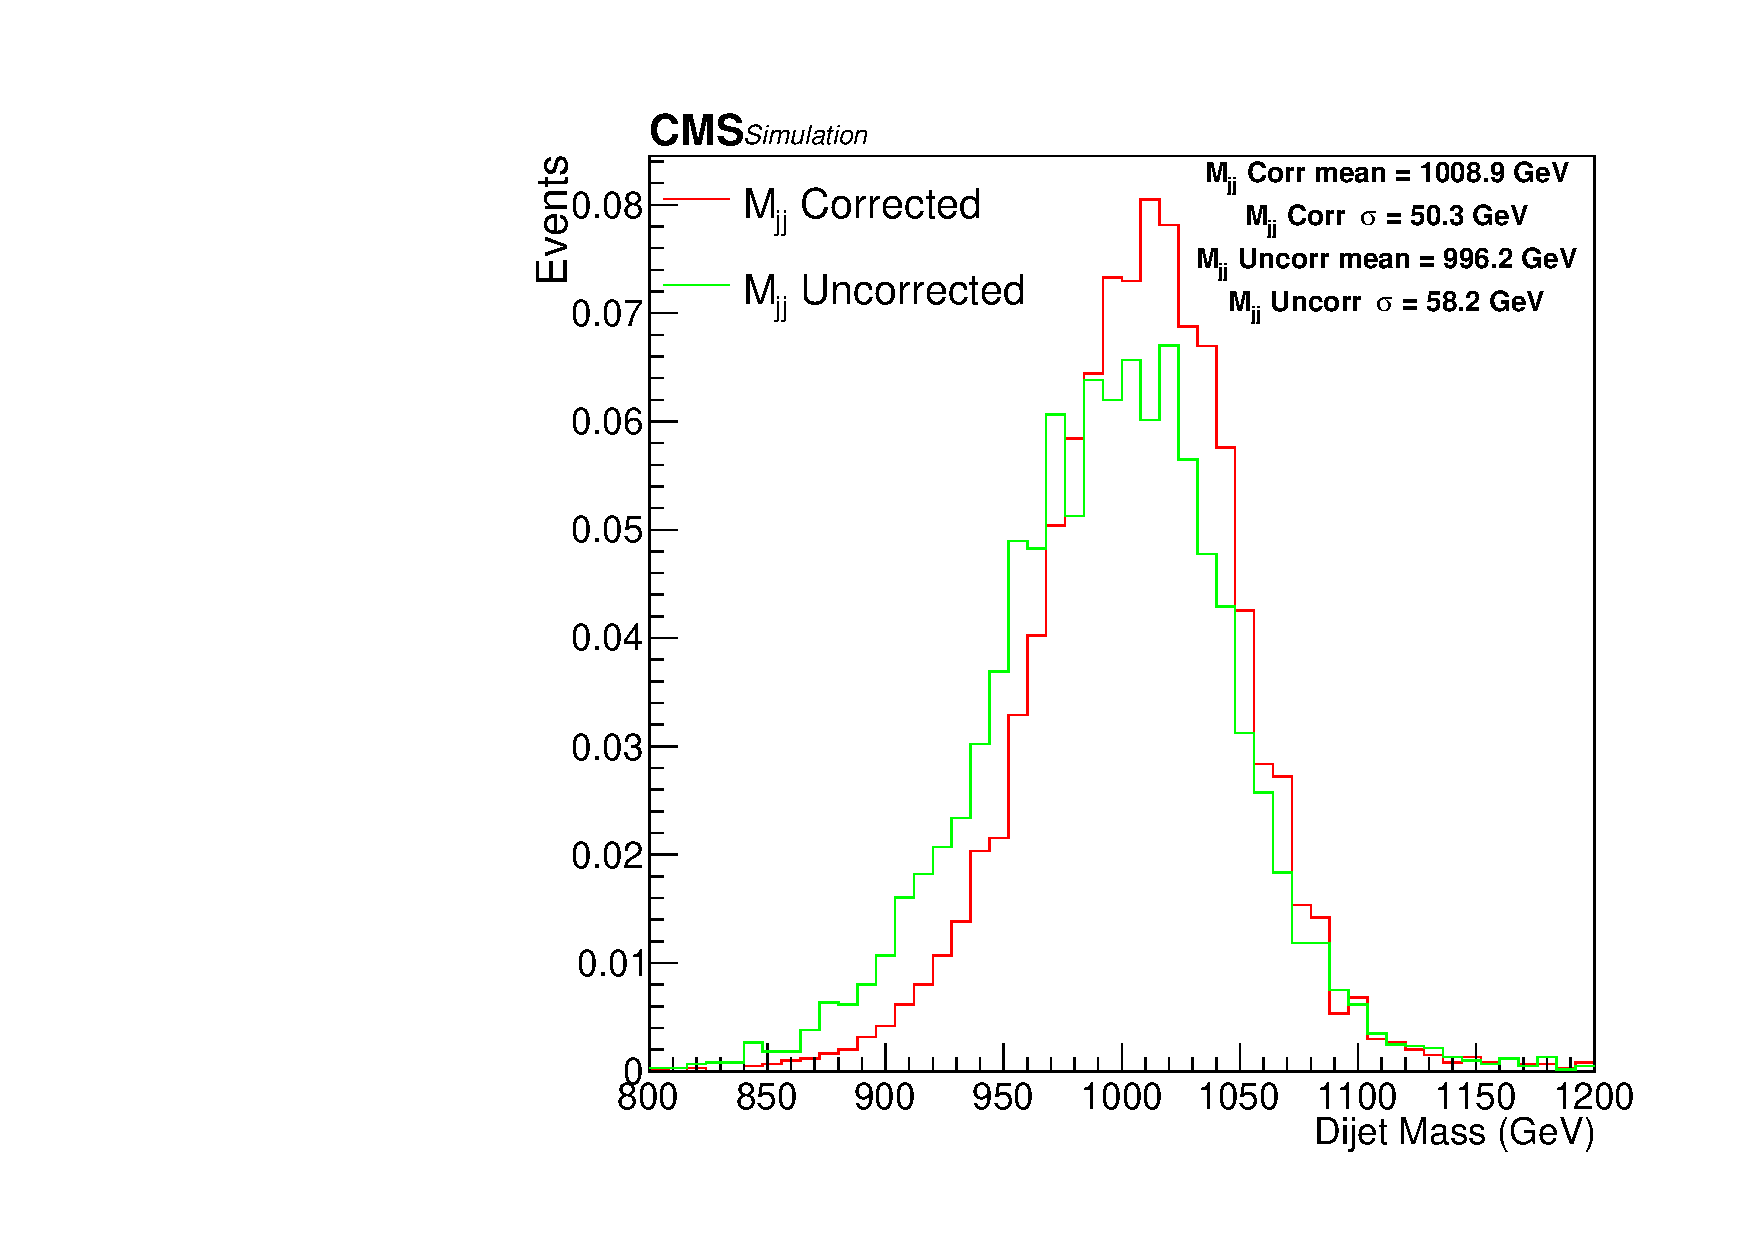
\includegraphics[scale=0.34]{Analysis/EventSelection/BulkGrav_M-1000_DijetMassCorrection_update.pdf}
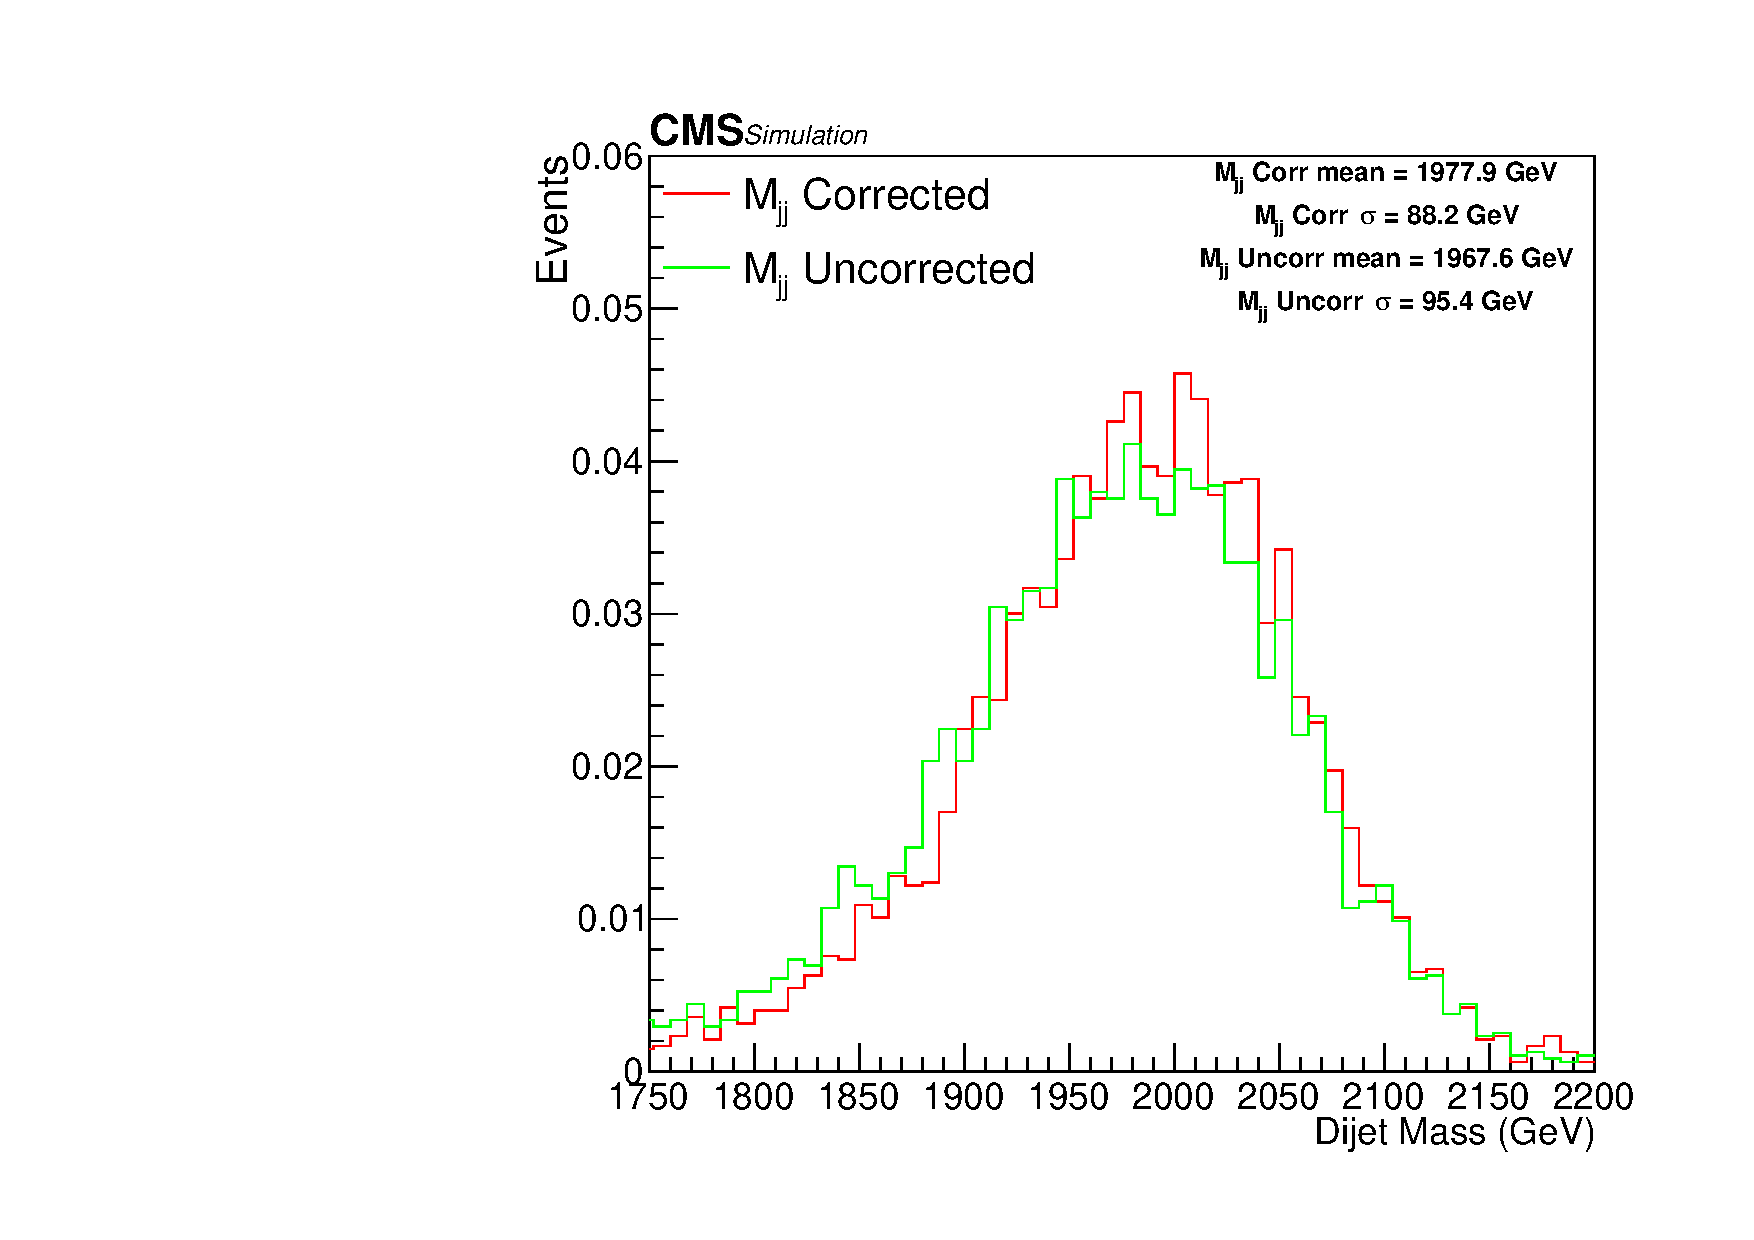
\includegraphics[scale=0.34]{Analysis/EventSelection/BulkGrav_M-2000_DijetMassCorrection_update.pdf}
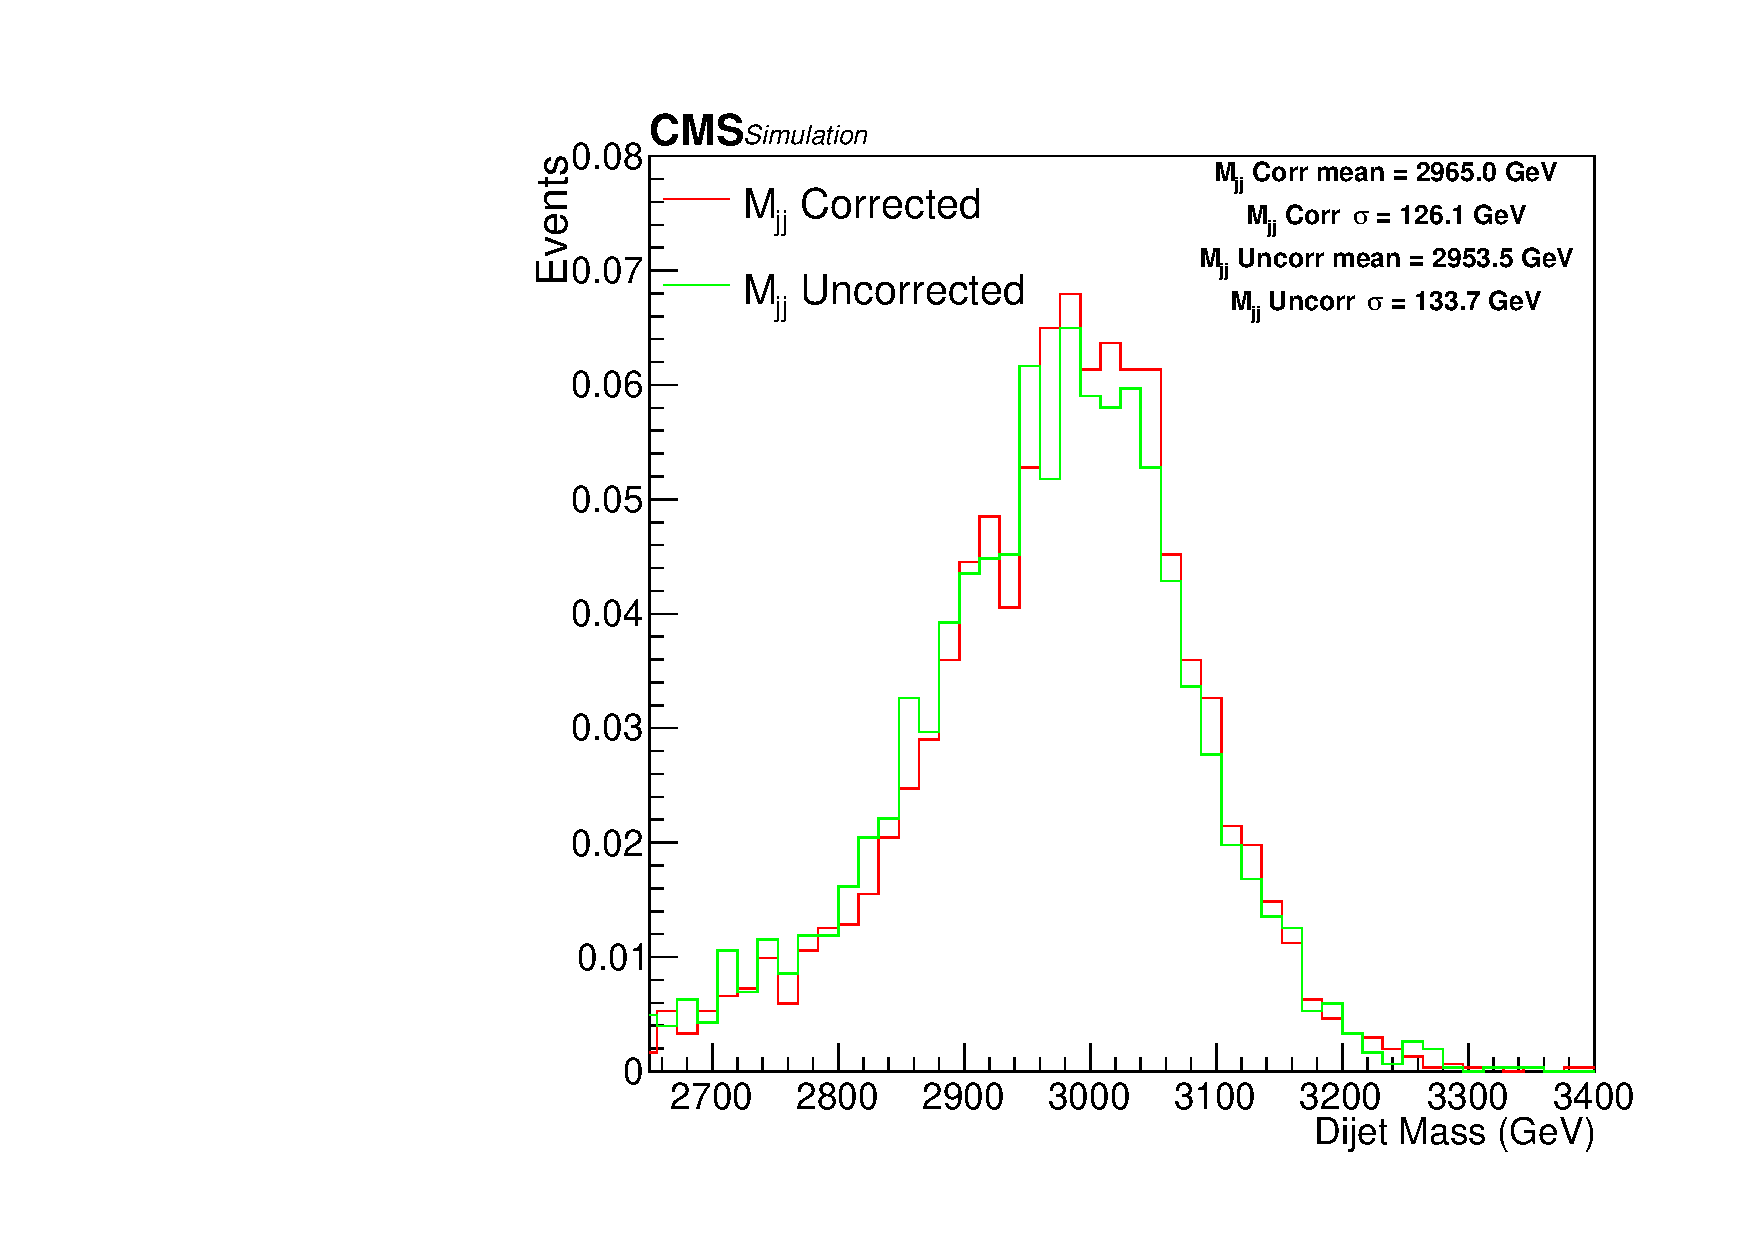
\includegraphics[scale=0.34]{Analysis/EventSelection/BulkGrav_M-3000_DijetMassCorrection_update.pdf}
\end{center}
\caption{The dijet mass distribution computed as described in Eqn.~\ref{eq:Mjjs} and compared to the standard dijet invariant mass for simulated signal events. The simulated Bulk Graviton mass points are 1000 (top left), 2000 (top right), and 3000 (bottom) GeV.}
\label{fig:subtImp}
\end{figure}

\subsection{Full Selection}

We compare the simulated distributions from QCD background and from signal after
applying the pre-selection criteria in Table~\ref{tab:datamcselection}; note the
b-tagging is not applied. In addition, when comparing a variable X, such as
$\tau_{21}^\mathrm{PUPPI}$, the pre-selection criterion on this variable is removed.
The cross sections of the QCD HT-binned MC in Section~\ref{sec:Samples} are known
to be imprecise, therefore, we normalize the number of events in simulation
according to the integrated luminosity of $35.9~\mathrm{fb}^{-1}$ with an additional correction
factor of 0.7, which is based on the data/MC scaling observed for QCD MC in 2015
analysis, to match the event yields in MC to that in the data.
Figures~\ref{fig:eventToplogy_prebtag}--\ref{fig:doublesv_prebtag} present the comparison of the
distributions of the simulated QCD events for the kinematic, jet substructure, and b-tagger variables of
the Higgs-jets, with those from bulk graviton with a resonance mass of 1.4, 1.8, and 2.5 TeV. For this comparison, a signal cross section of 20~pb is assumed for each signal mass point. The simulated QCD events are further subdivided into different categories based the matched hadron flavor as listed in Table~\ref{tab:qcdflavor}.


\begin{table}[htb]
\begin{center}
    \begin{tabular}{l l}
    \hline
    \hline
    Variable &  Cut \\
    \hline
    Trigger &  Section~\ref{ss:trigger}\\
    Lepton veto & Section~\ref{sec:EvtSel} \\
    Number of good vertices & $\geq 1$ \\
    Tight PF jet ID in Table~\ref{tab:tightjetid} & Pass  \\
    Higgs jet $p_{T}$ & $>300$ GeV \\
    Higgs jet $\left|\eta\right|$ & $<2.4$ \\
    $|\Delta\eta_{jj}|$ & $<1.3$ \\
    $M_{jj}^{red}$ & $>750$ GeV \\
    Thea-corrected puppi-softdrop mass, $M_{soft-drop}$ & $105-135$ GeV \\
    $\tau_{21}^\mathrm{PUPPI}$ & $<0.55$ \\
    \hline
    \hline
    \end{tabular}
    \caption[Pre-selection criteria for the comparison of MC distributions.]{Pre-selection criteria for the comparison of MC distributions. \label{tab:datamcselection}}
\end{center}
\end{table}

\begin{table}[htb]
\begin{center}
    \begin{tabular}{c c c}
    \hline
    \hline
    Label in Figures &  hadron flavor ID of AK8 jets & hadron flavor ID of sub-jets  \\
    \hline
    bb & 5 & 5 (both) \\
    b & 5 & 5 (only one) \\
    cc / c & 4 & 4 (at least one) \\
    udsg & all remaining & all remaining \\
    \hline
    \hline
    \end{tabular}
    \caption[The categorization of simulated QCD events.]{The categorization of simulated QCD events. \label{tab:qcdflavor}}
\end{center}
\end{table}

\begin{figure}[H]
\centering
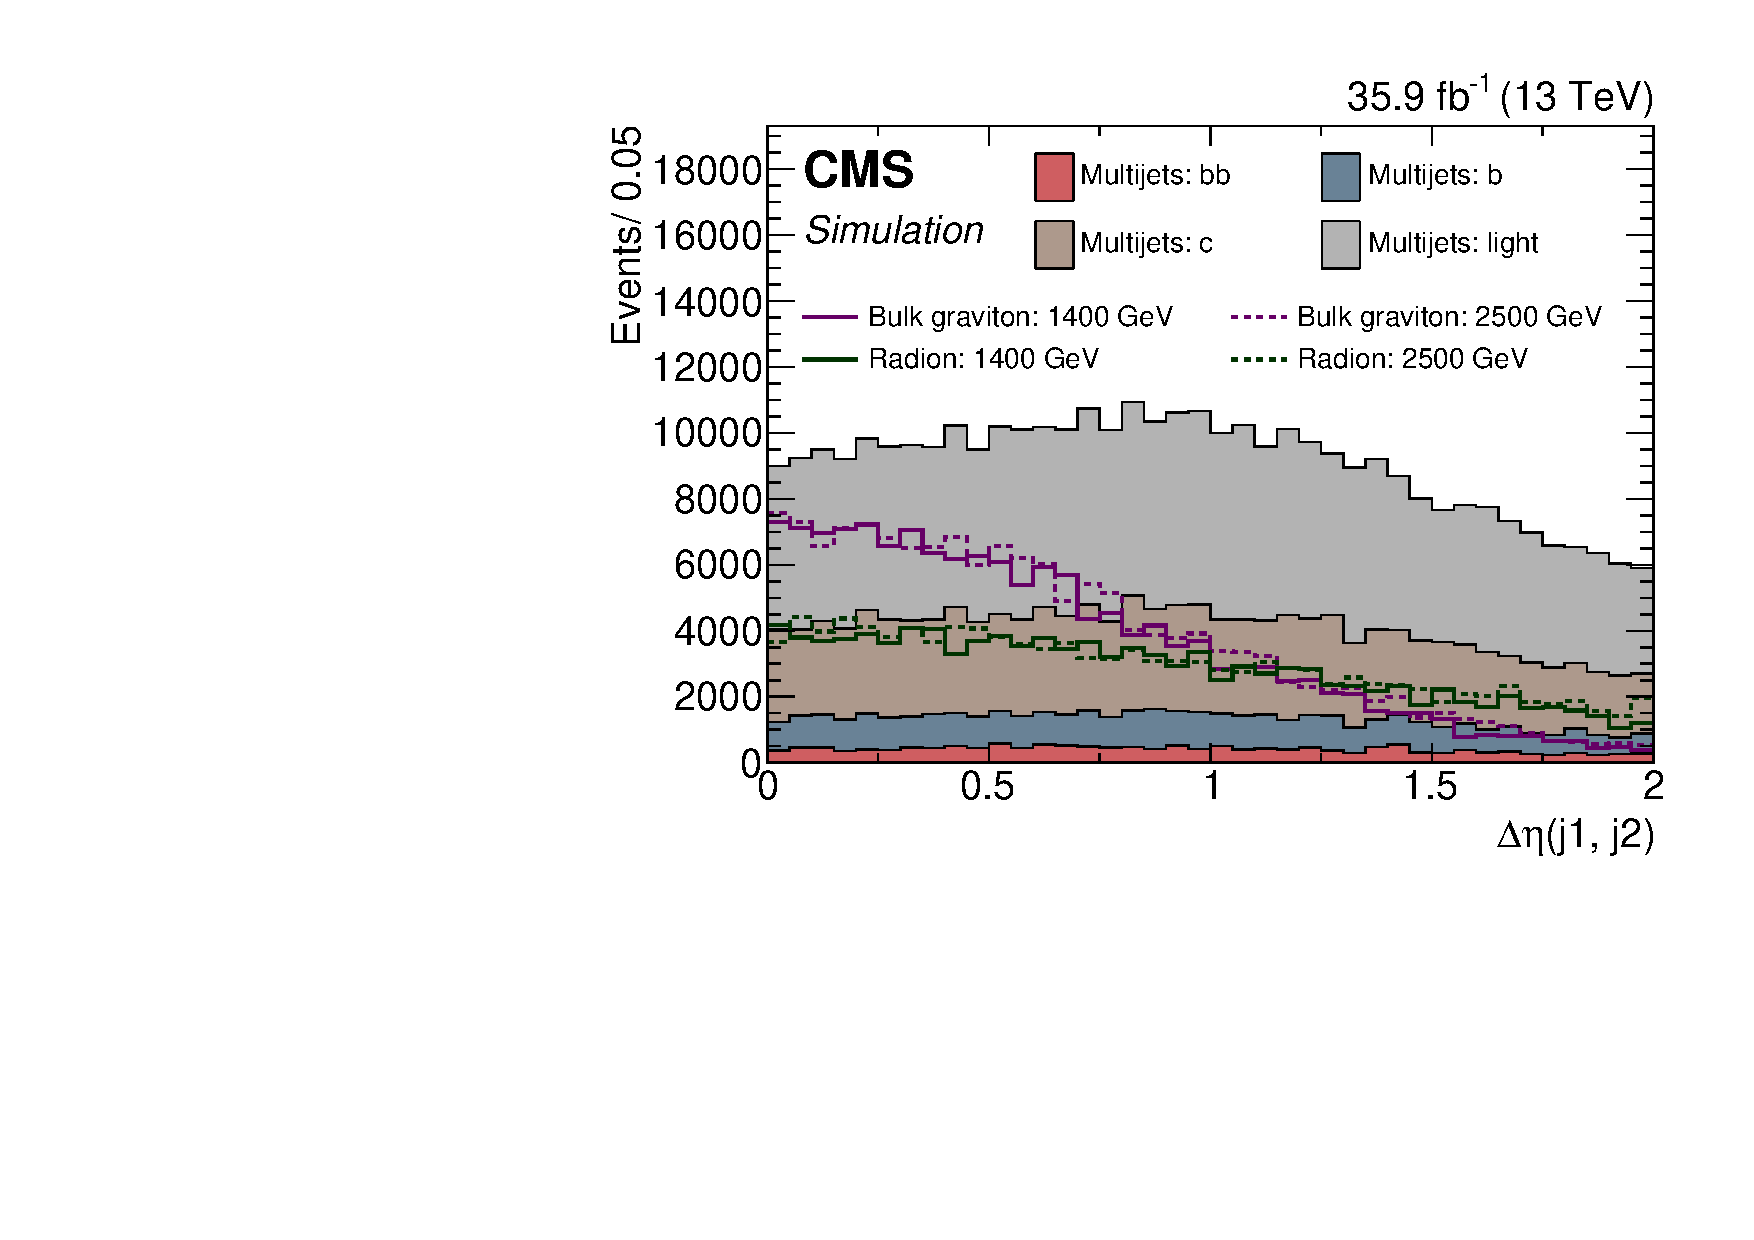
\includegraphics[width=0.45\textwidth]{Analysis/EventSelection/cmc_deltaEta.pdf} \\
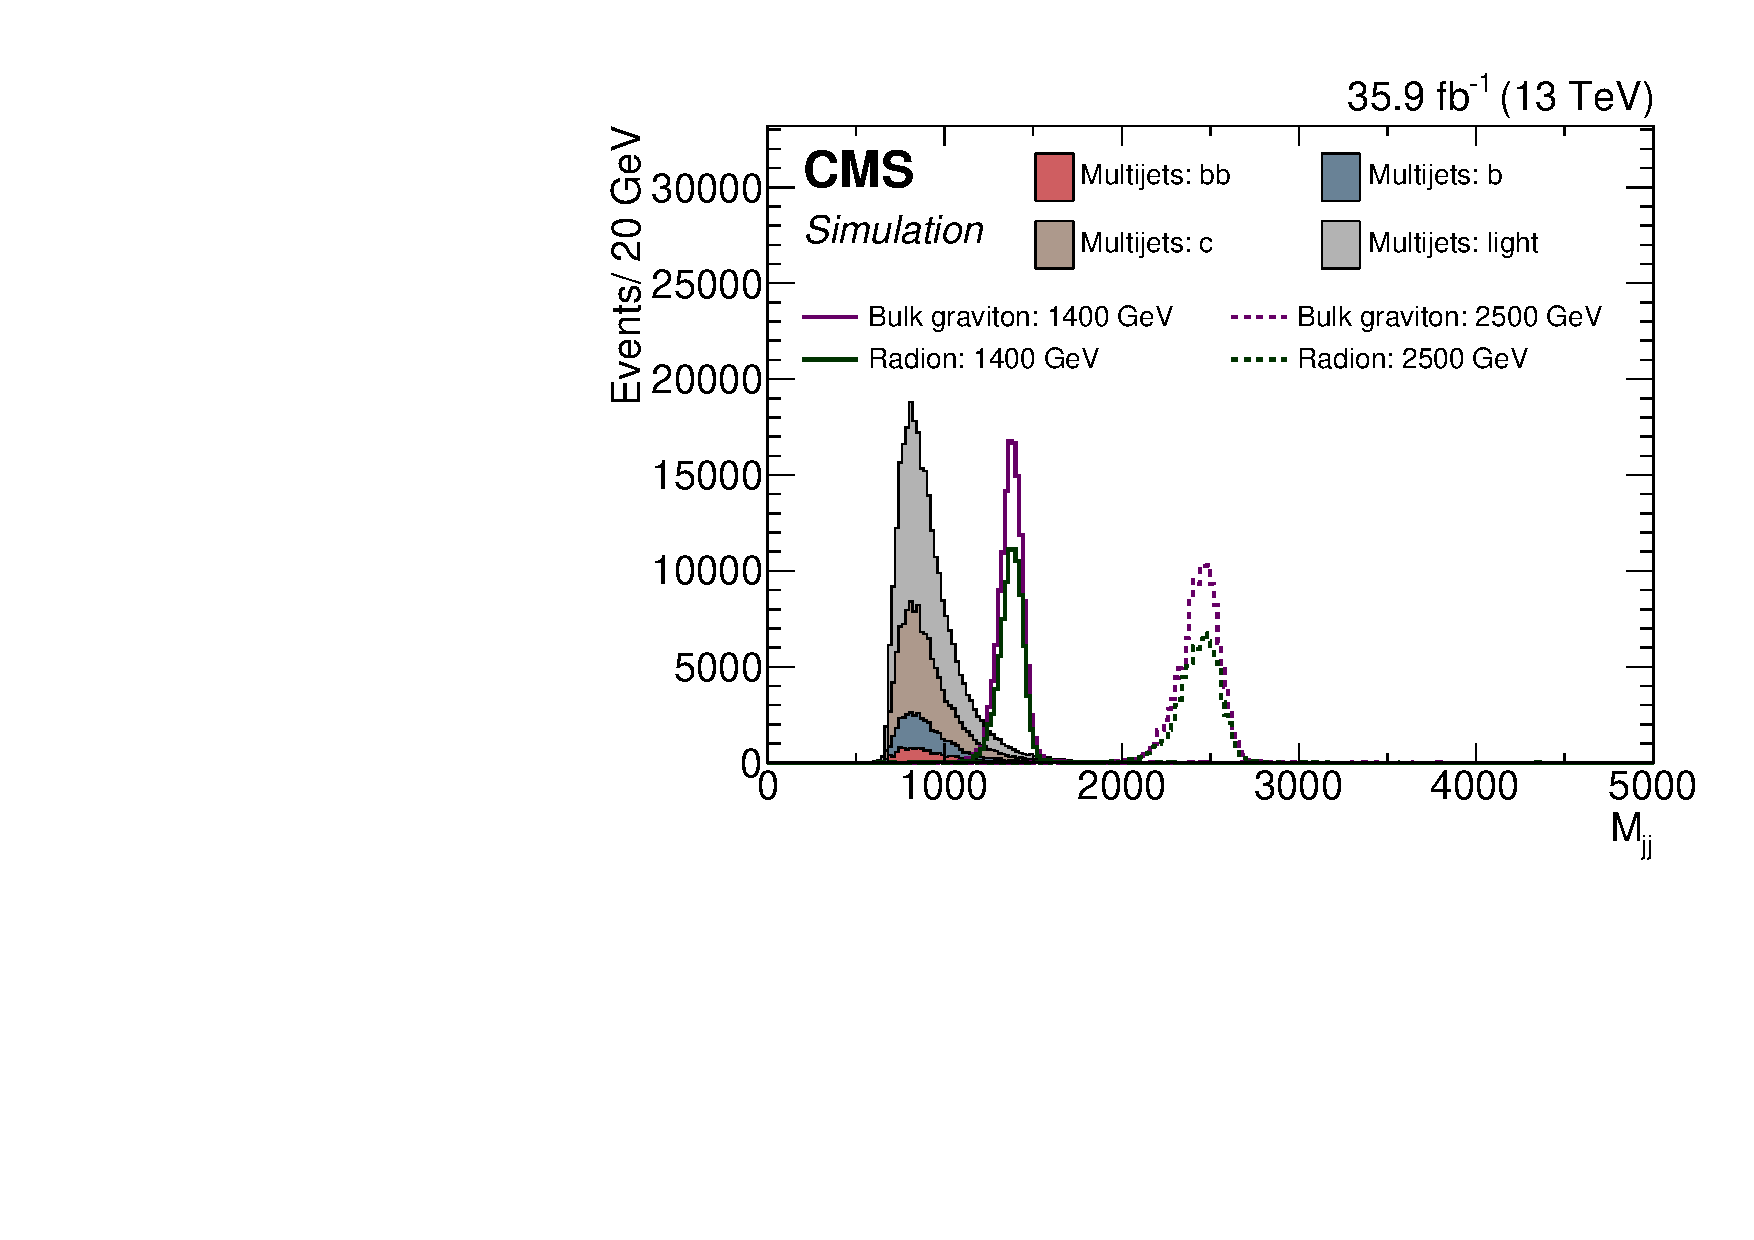
\includegraphics[width=0.45\textwidth]{Analysis/EventSelection/cmc_totalMass.pdf}
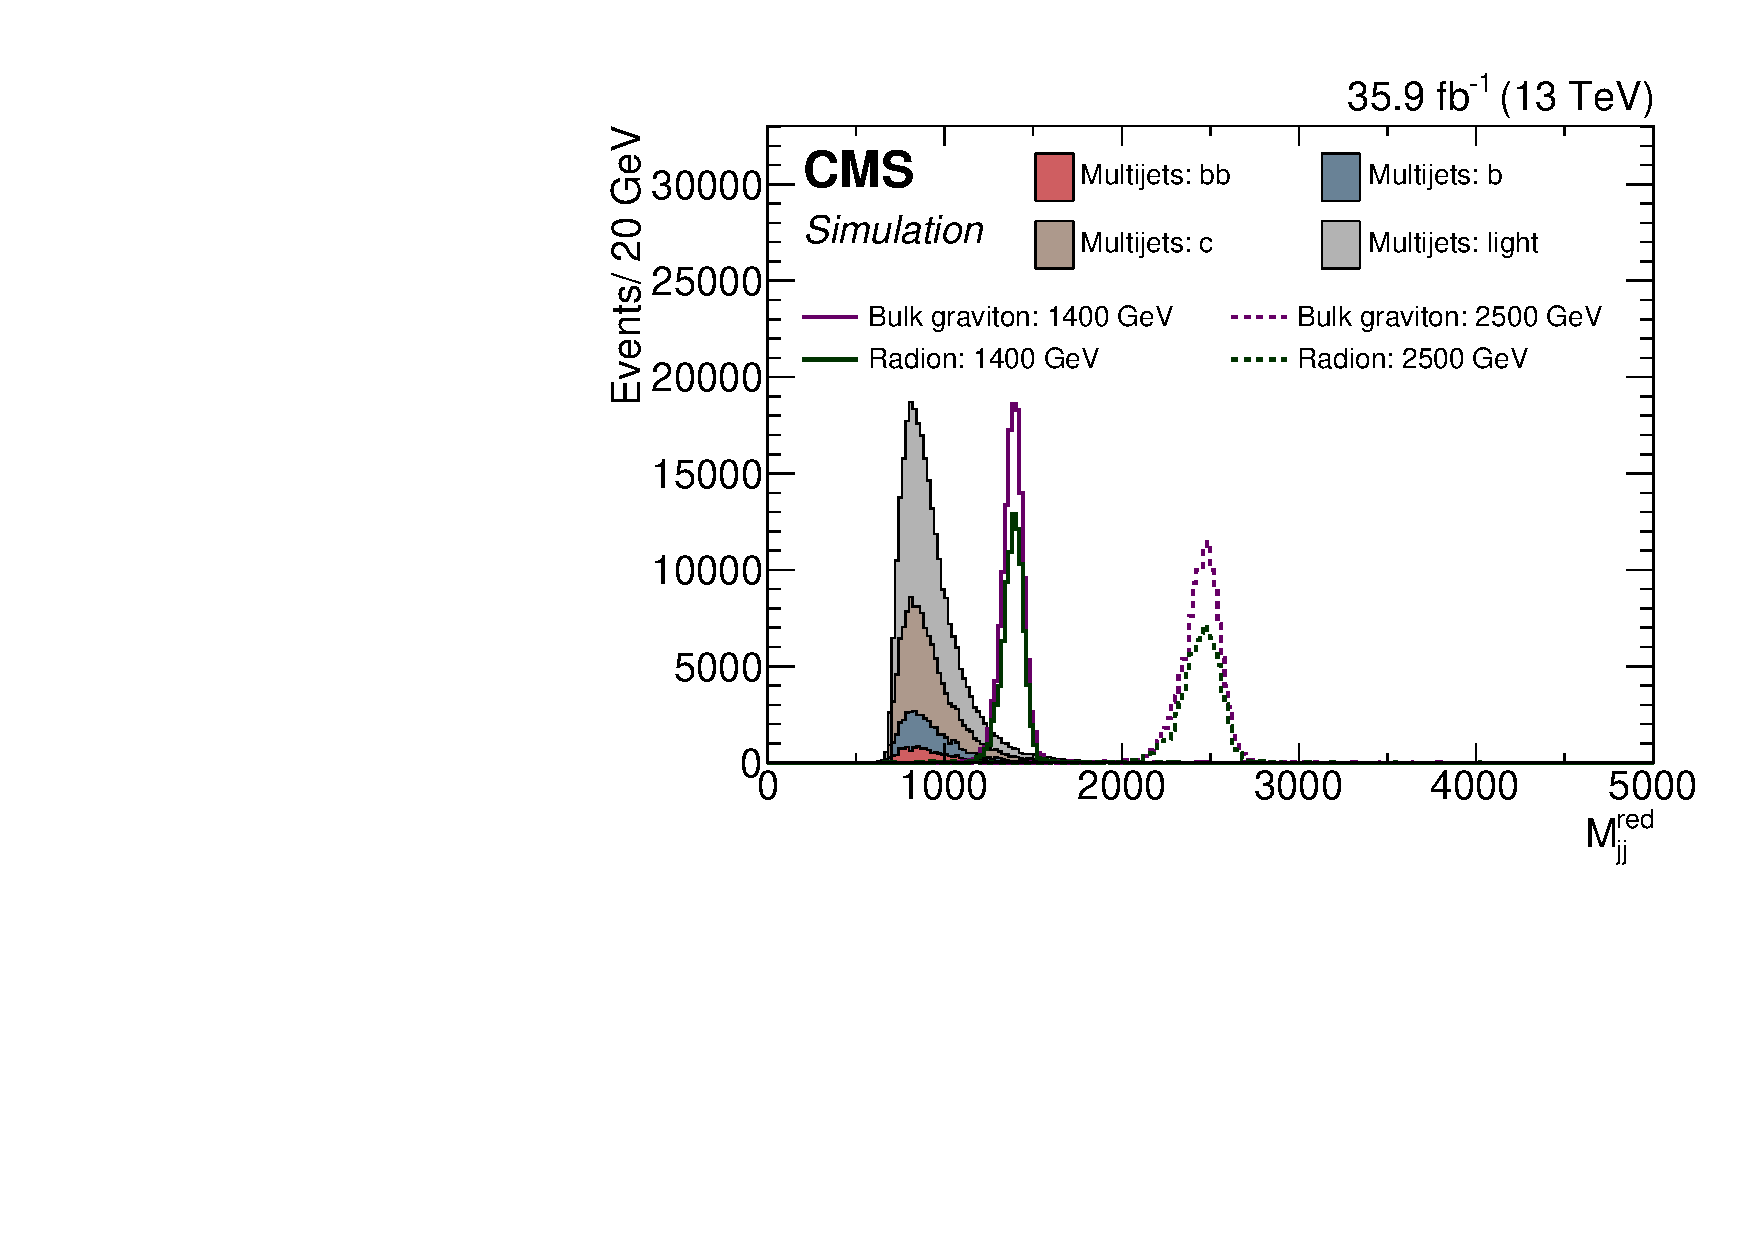
\includegraphics[width=0.45\textwidth]{Analysis/EventSelection/cmc_totalMassRed.pdf}
\caption{ Comparison of simulated events after pre-selection, $|\Delta\eta_{jj}|$ (upper), $M_{jj}$ (lower left), and $M_{jj}^{red}$ (lower right). A signal cross section of 20~pb is assumed for each signal mass point.
\label{fig:eventToplogy_prebtag}
}
\end{figure}

\begin{figure}[H]
\centering
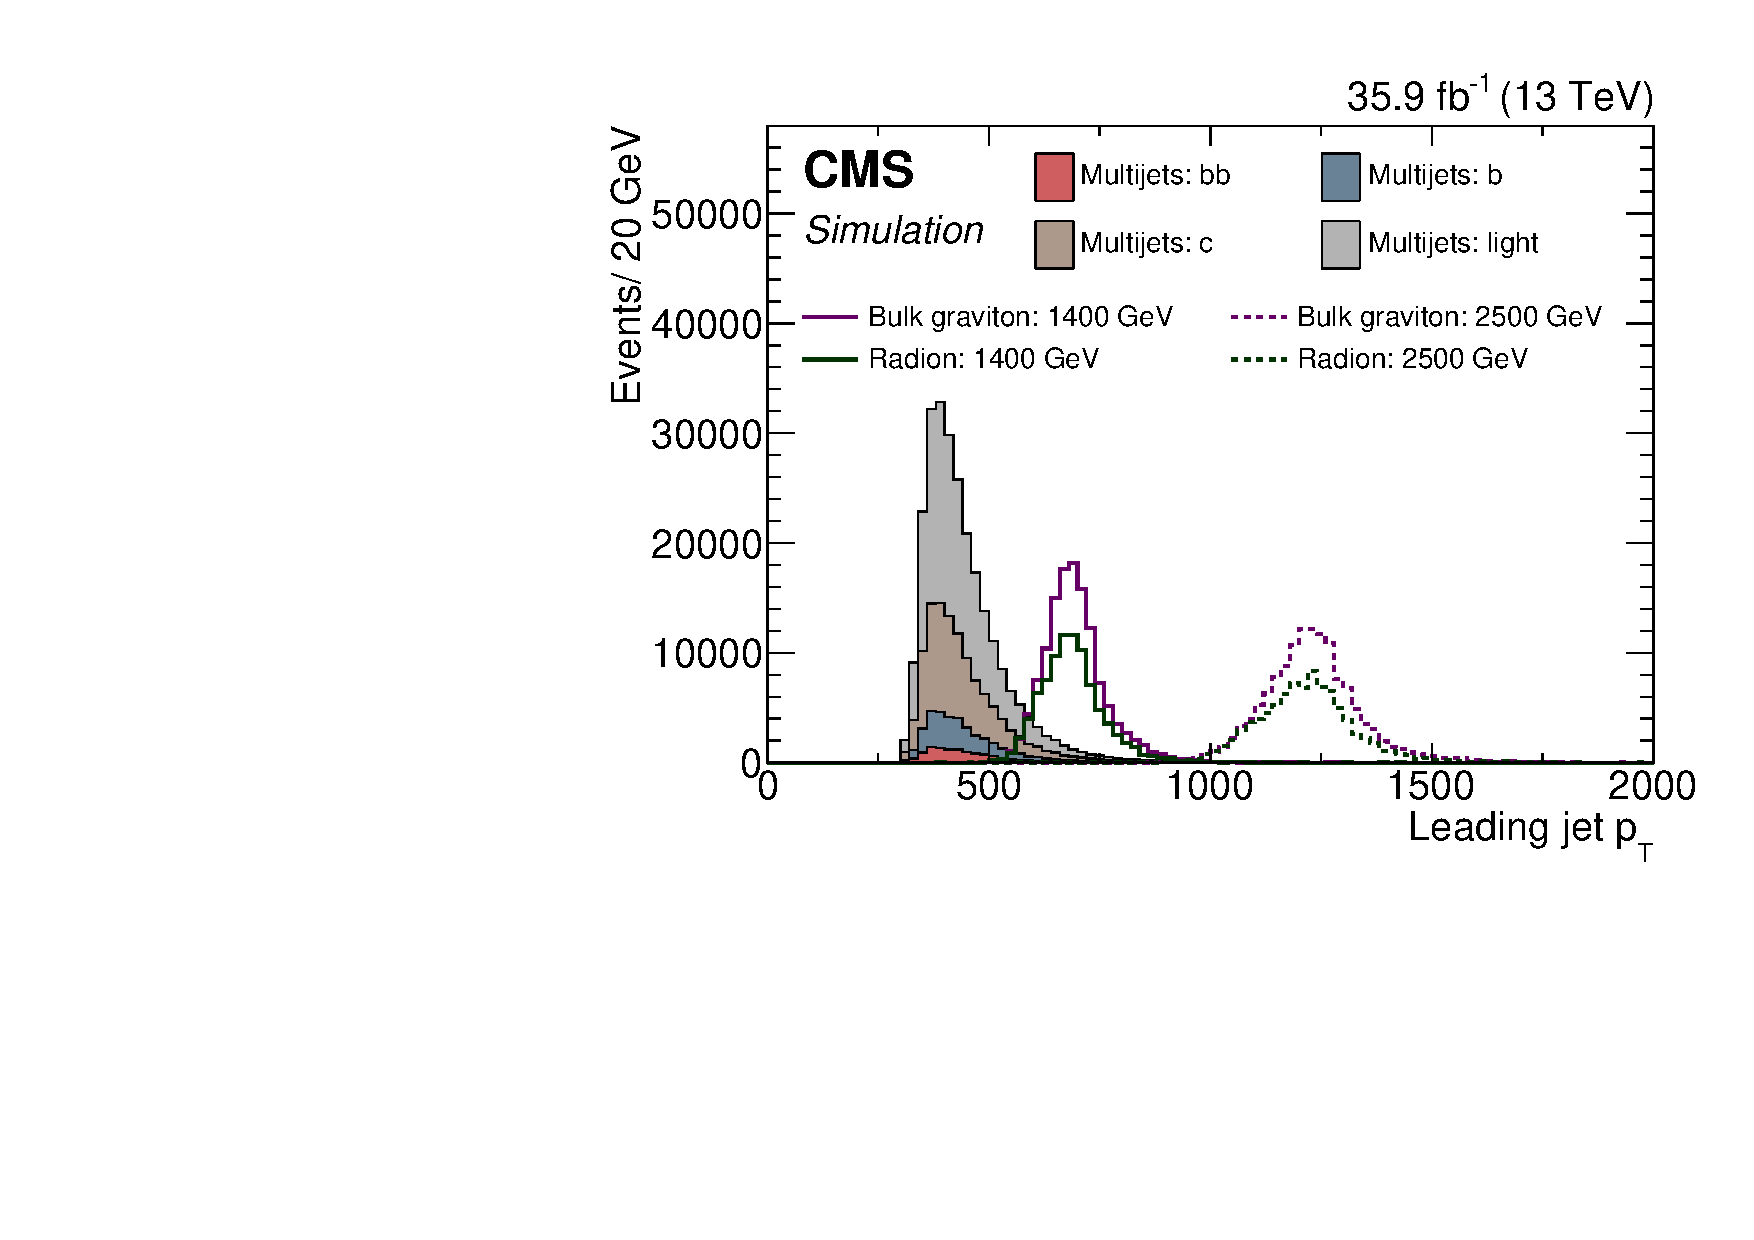
\includegraphics[width=0.45\textwidth]{Analysis/EventSelection/cmc_pt_j0.pdf}
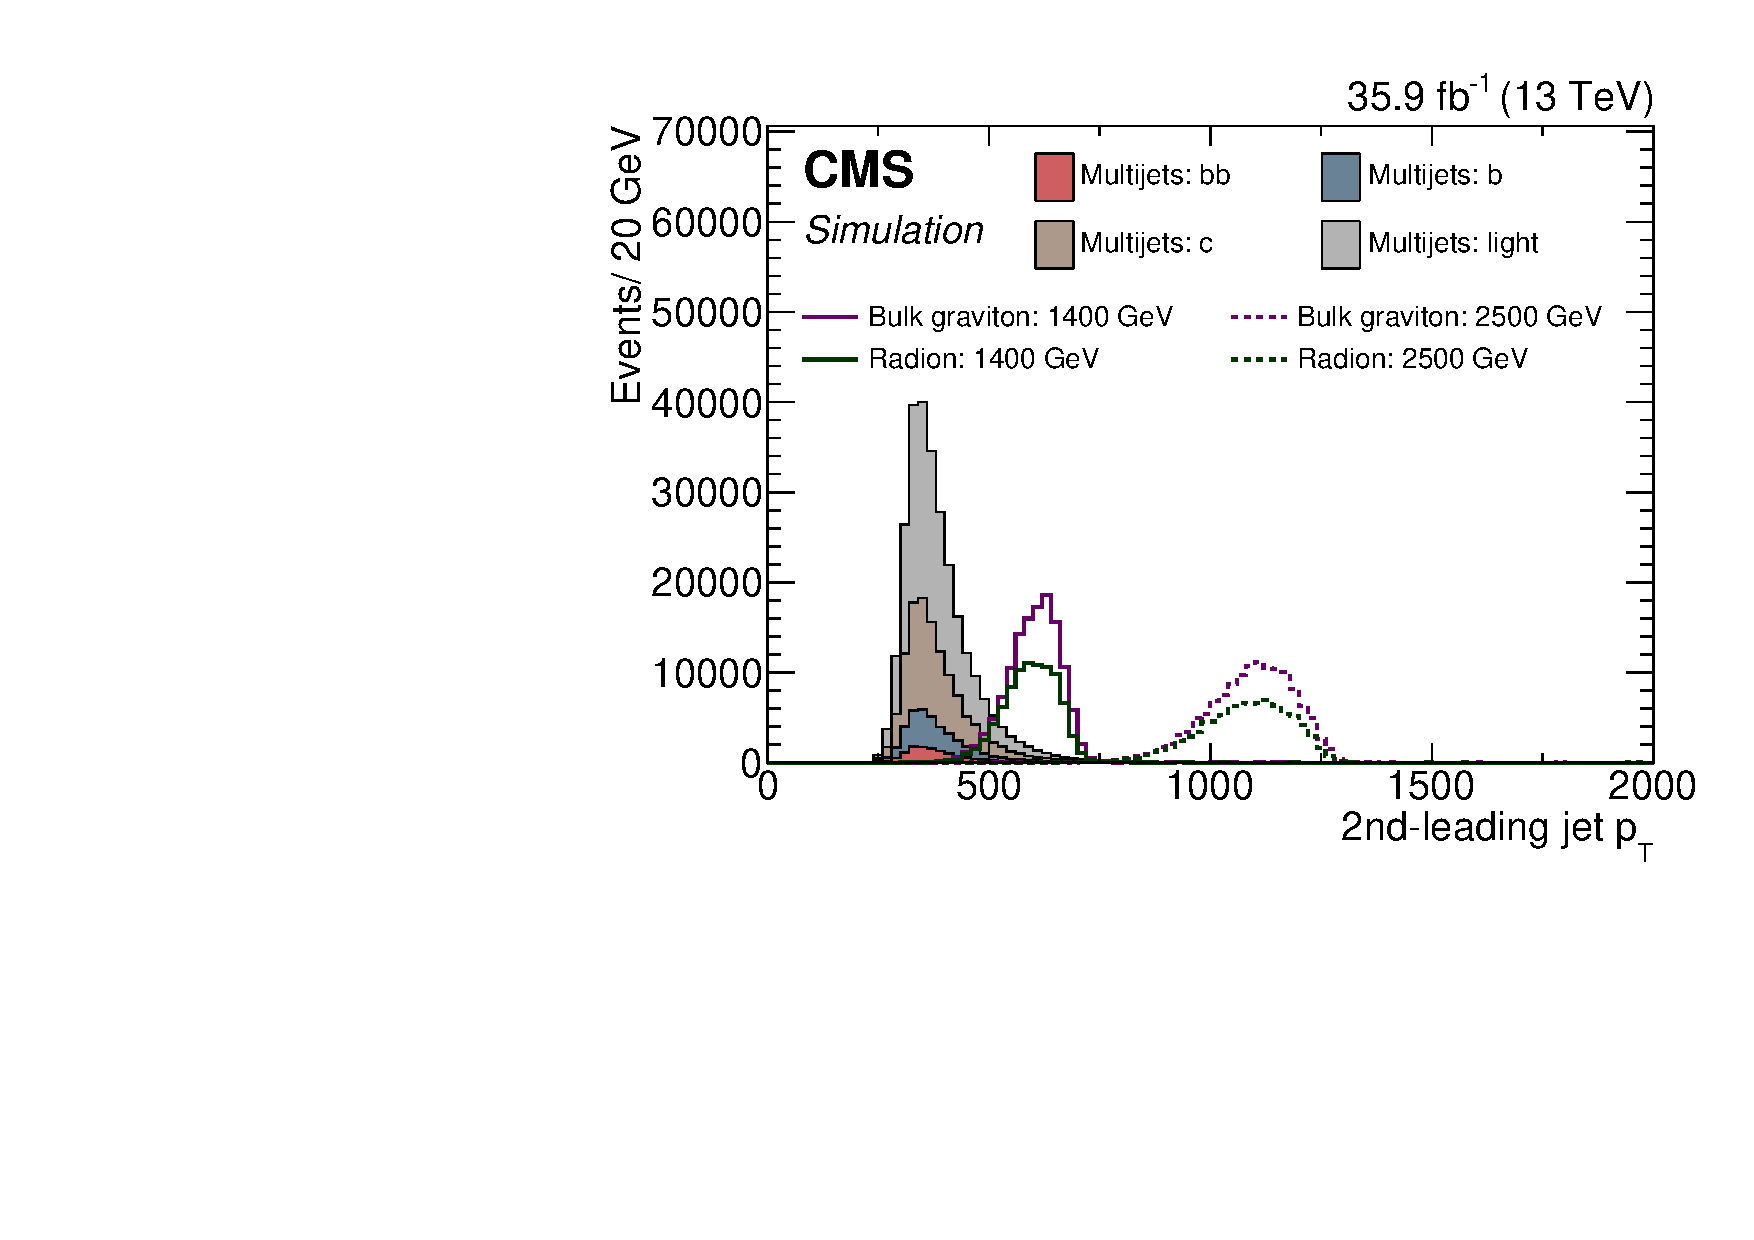
\includegraphics[width=0.45\textwidth]{Analysis/EventSelection/cmc_pt_j1.pdf} \\
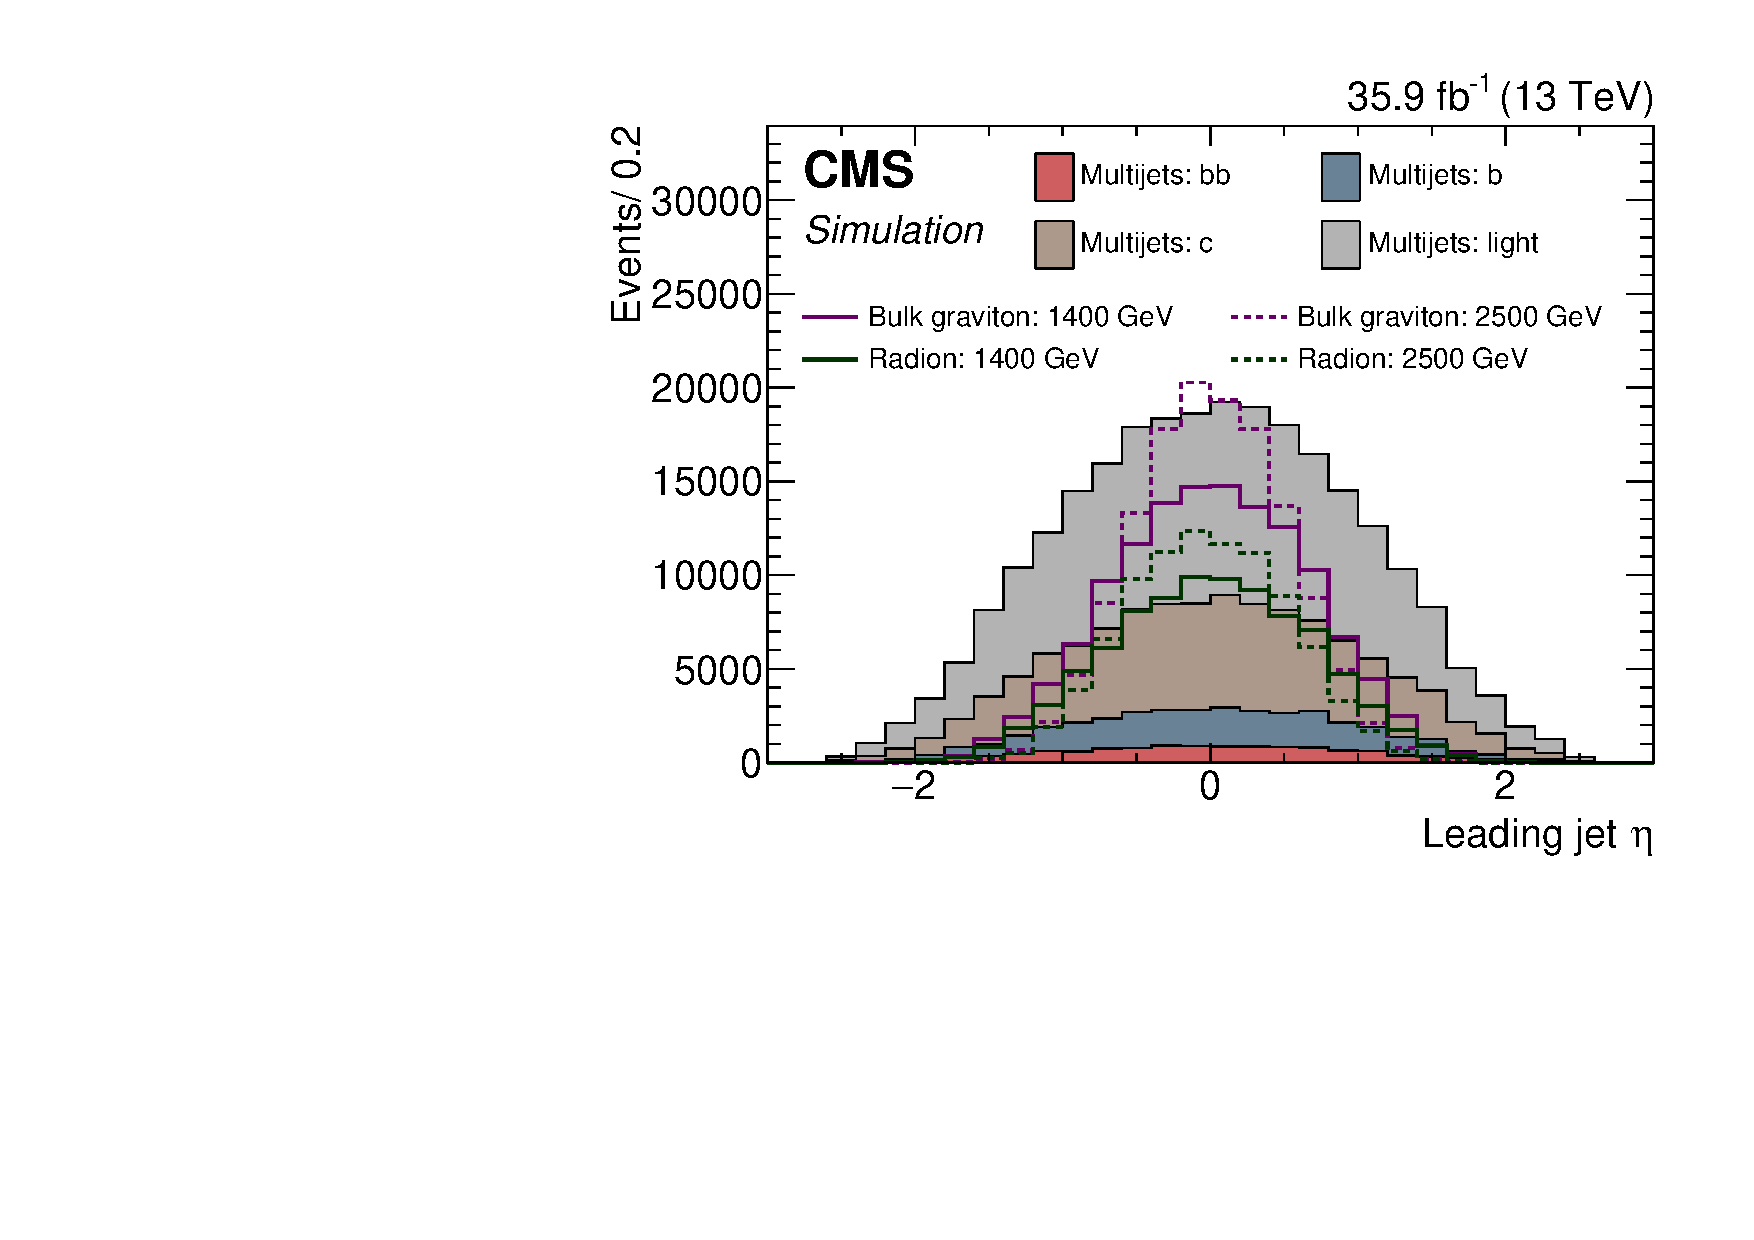
\includegraphics[width=0.45\textwidth]{Analysis/EventSelection/cmc_eta_j0.pdf}
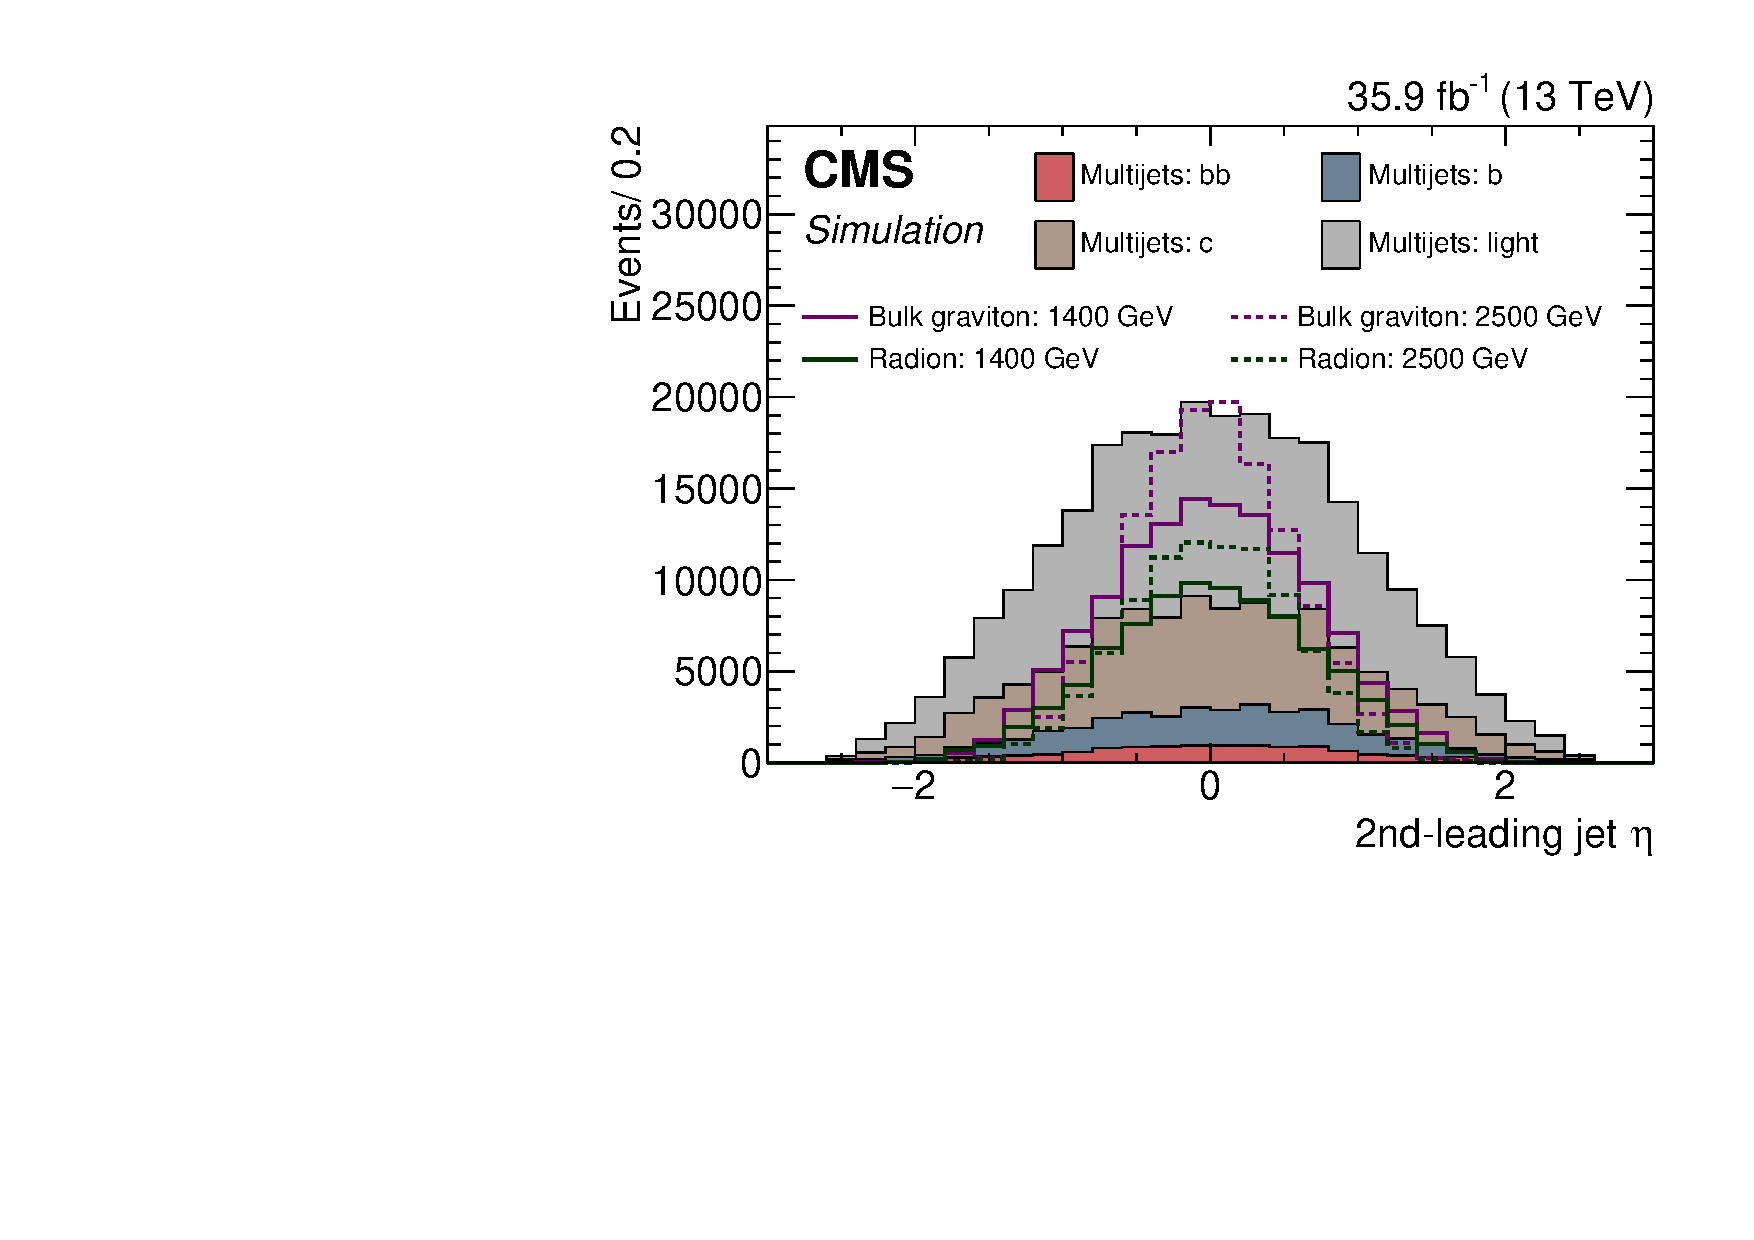
\includegraphics[width=0.45\textwidth]{Analysis/EventSelection/cmc_eta_j1.pdf}
\caption{ Comparison of simulated events after pre-selection, for the $p_{T}$ (upper) and $\eta$ (lower) of
 leading (left) and sub-leading (right) Higgs-jets.
A signal cross section of 20~pb is assumed for each signal mass point.
\label{fig:higgsjet_prebtag}
}

\end{figure}
\begin{figure}[H]
\centering
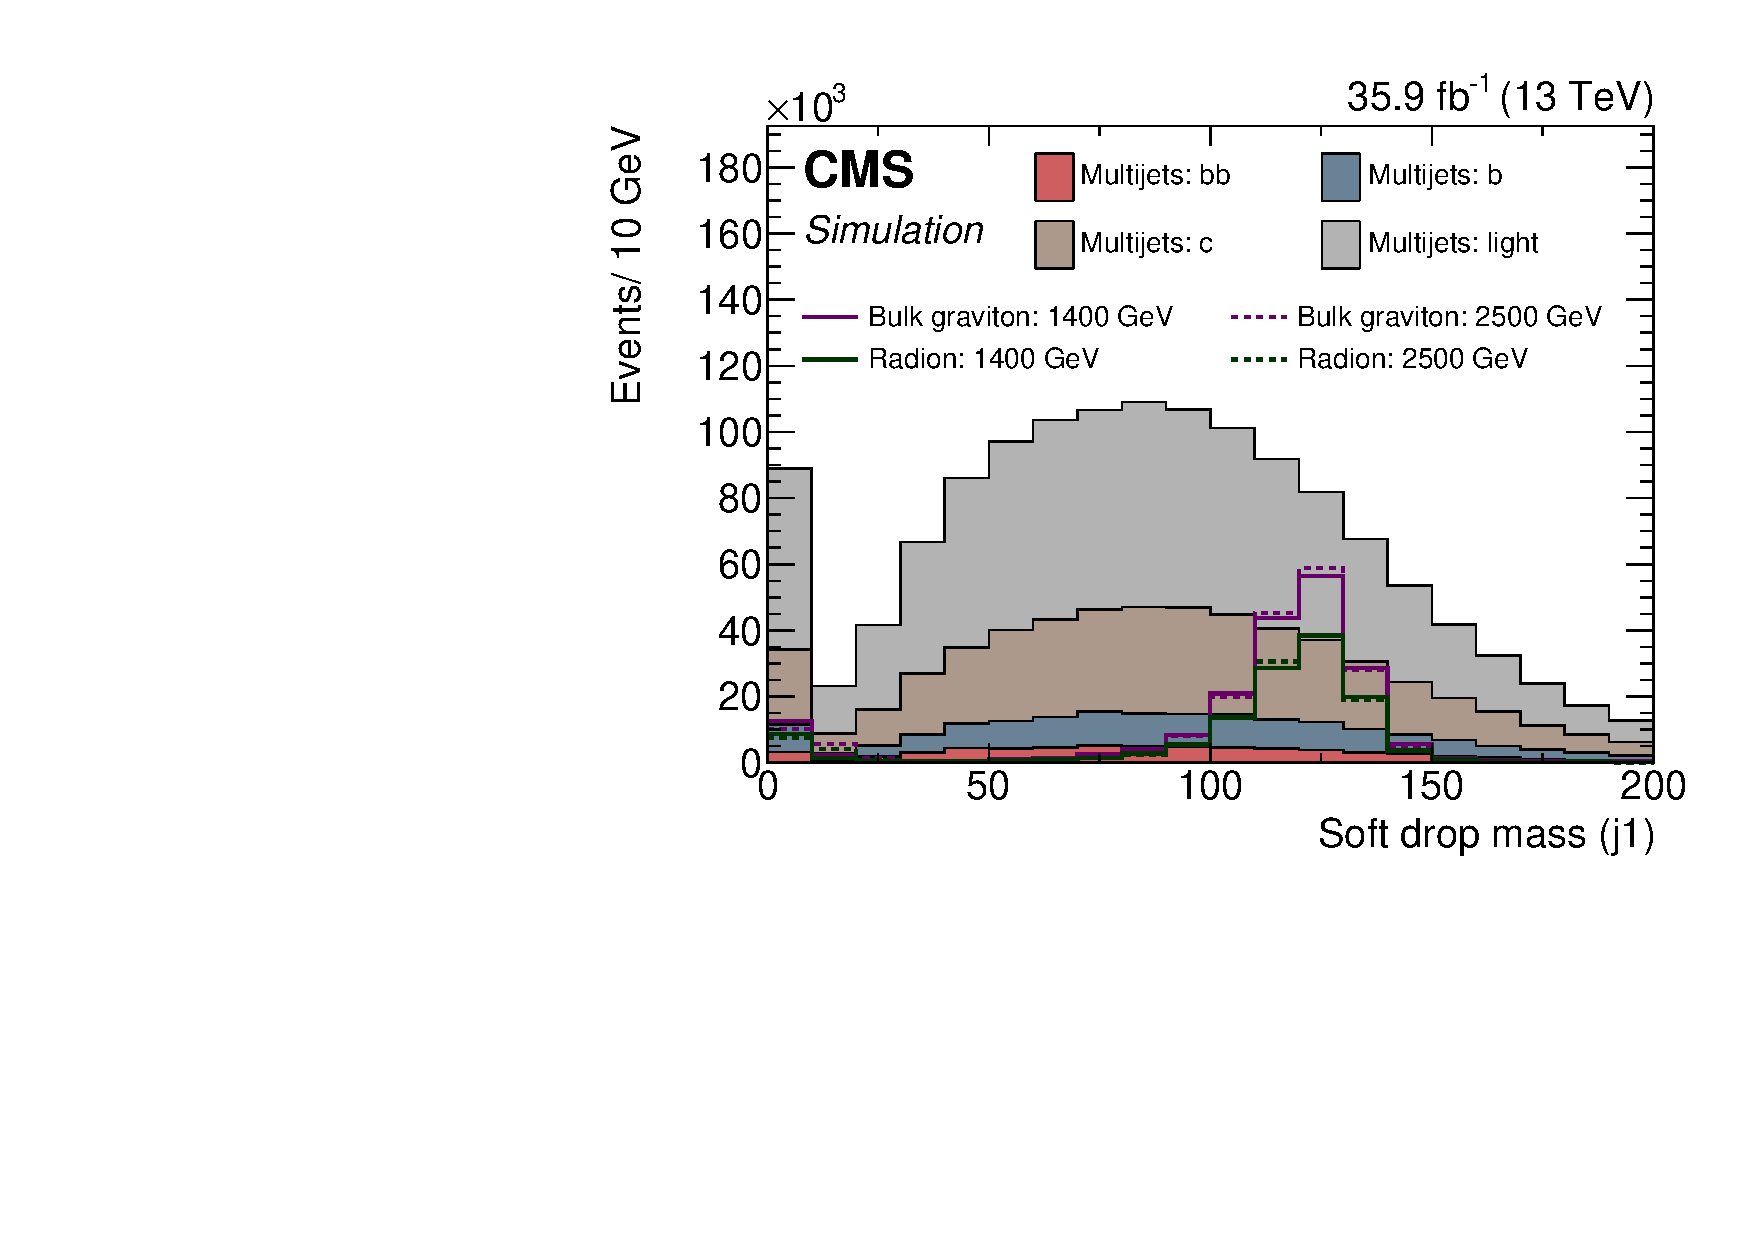
\includegraphics[width=0.45\textwidth]{Analysis/EventSelection/cmc_puppiSDMassThea_j0.pdf}
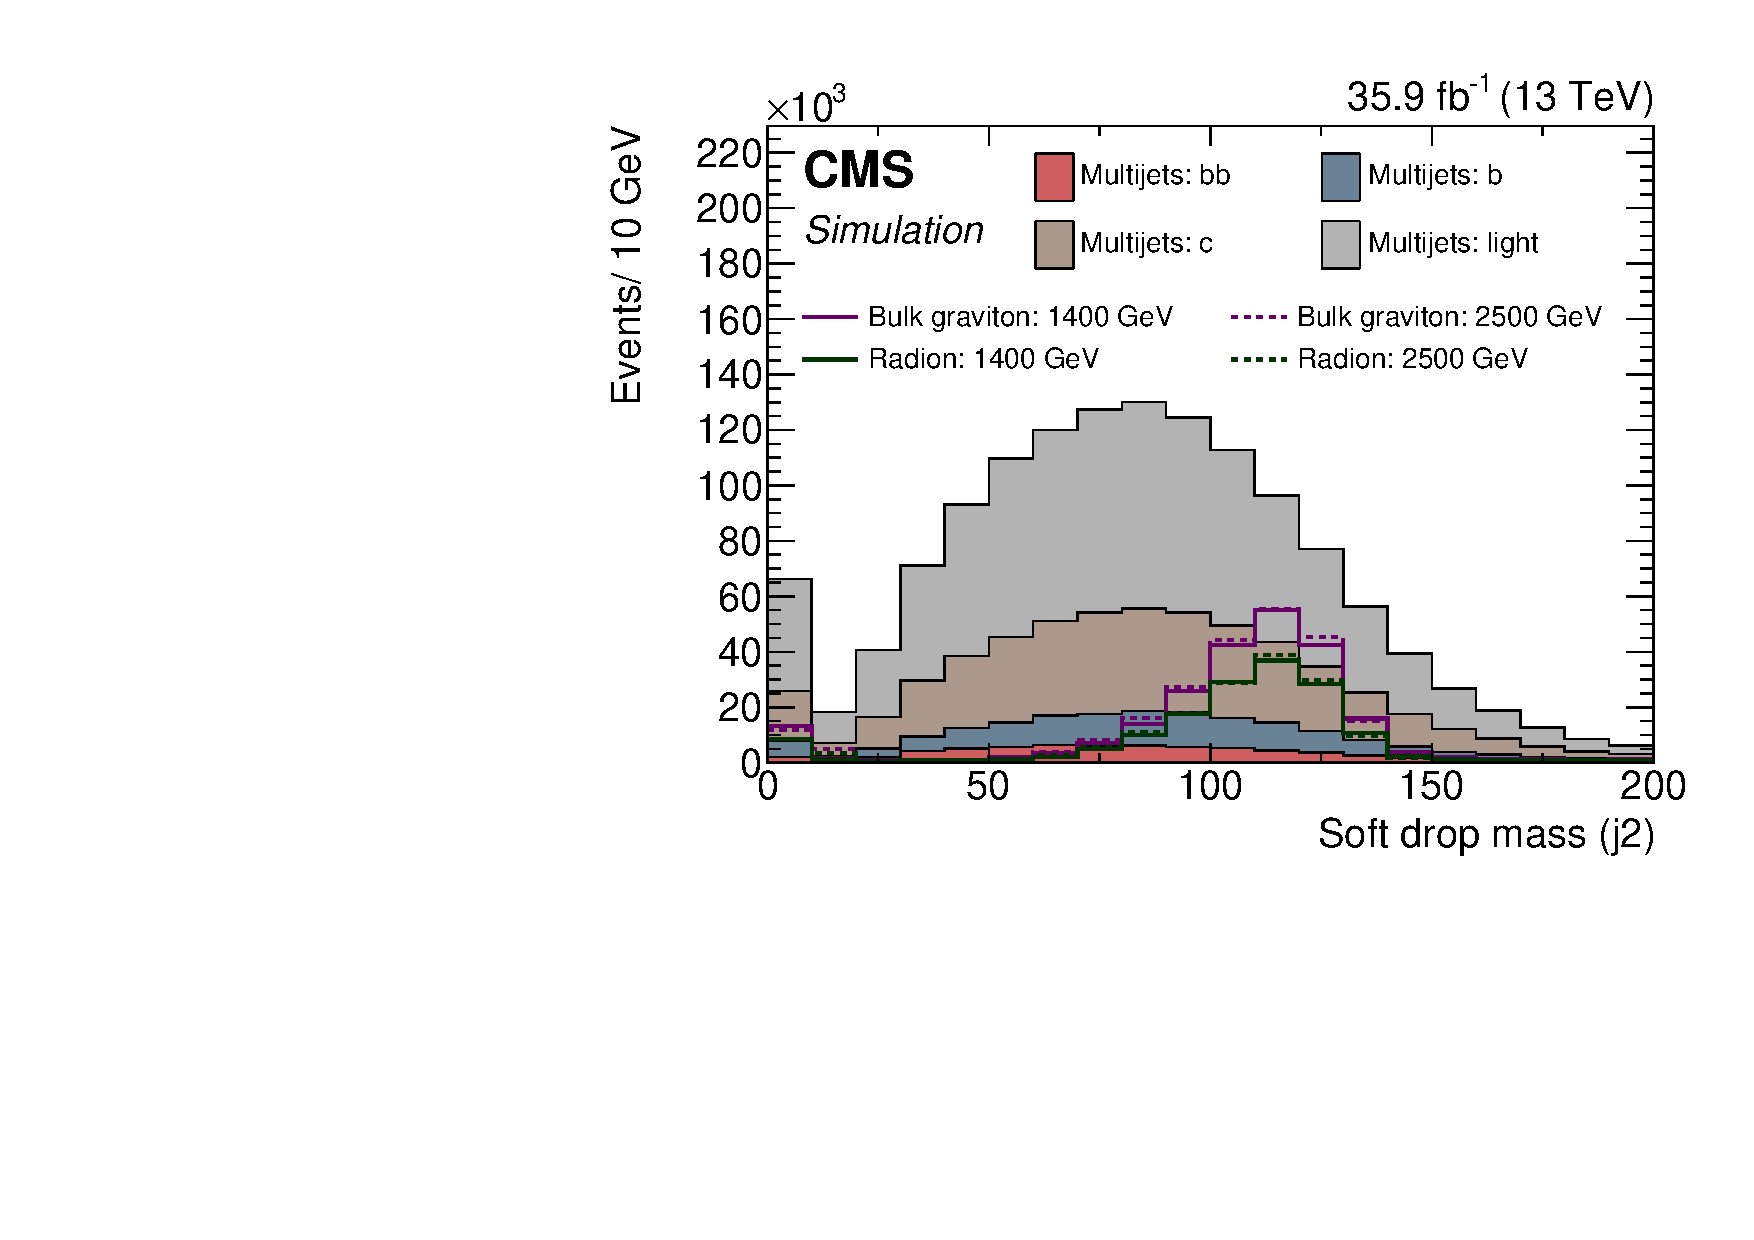
\includegraphics[width=0.45\textwidth]{Analysis/EventSelection/cmc_puppiSDMassThea_j1.pdf} \\
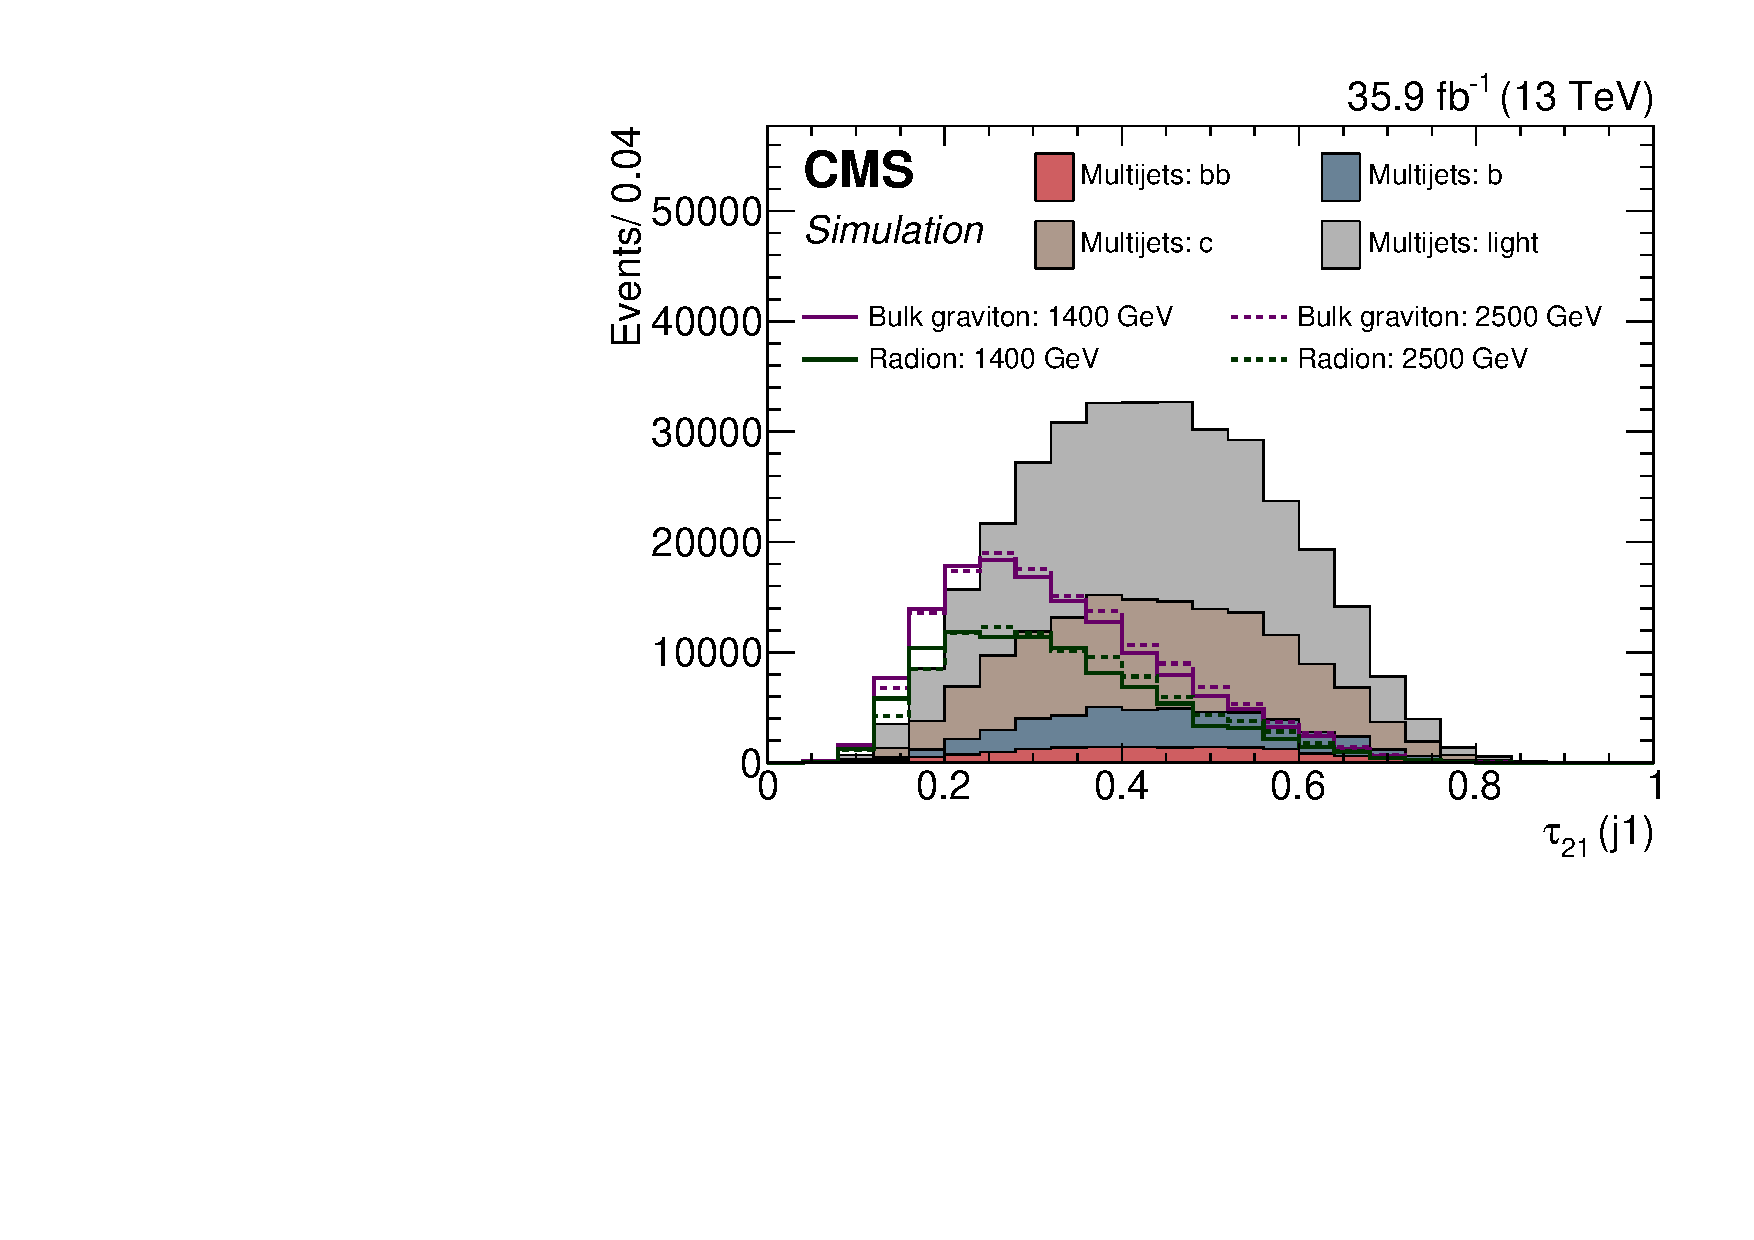
\includegraphics[width=0.45\textwidth]{Analysis/EventSelection/cmc_puppiTau21_j0.pdf}
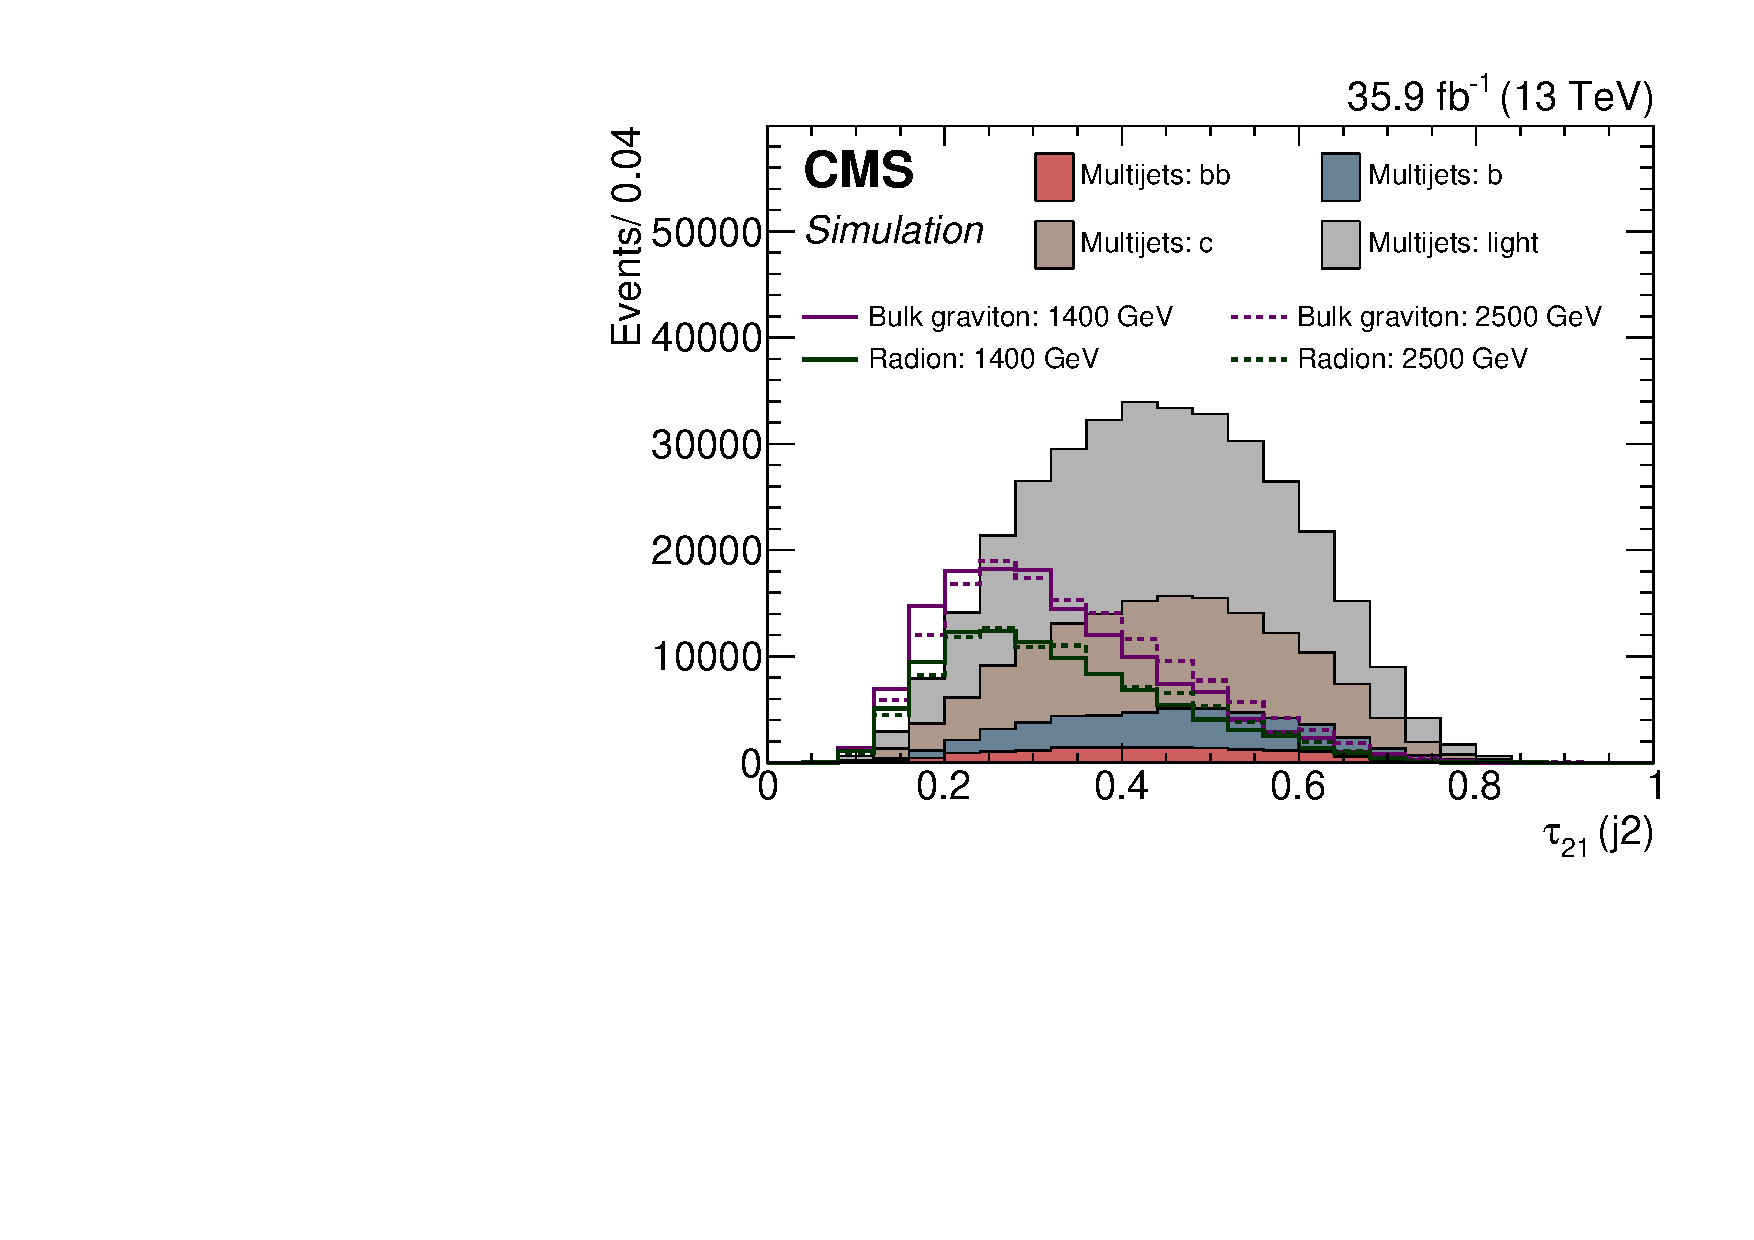
\includegraphics[width=0.45\textwidth]{Analysis/EventSelection/cmc_puppiTau21_j1.pdf}
\caption{ Comparison of simulated events after pre-selection, for the corrected Puppi+Softdrop mass (upper)
 and the $\tau_{21}^\mathrm{Puppi}$ (lower) of the leading (left) and sub-leading (right) Higgs-jets.
 A signal cross section of 20~pb is assumed for each signal mass point.
\label{fig:uncorrsd_prebtag}
}
\end{figure}

\begin{figure}[H]
\centering
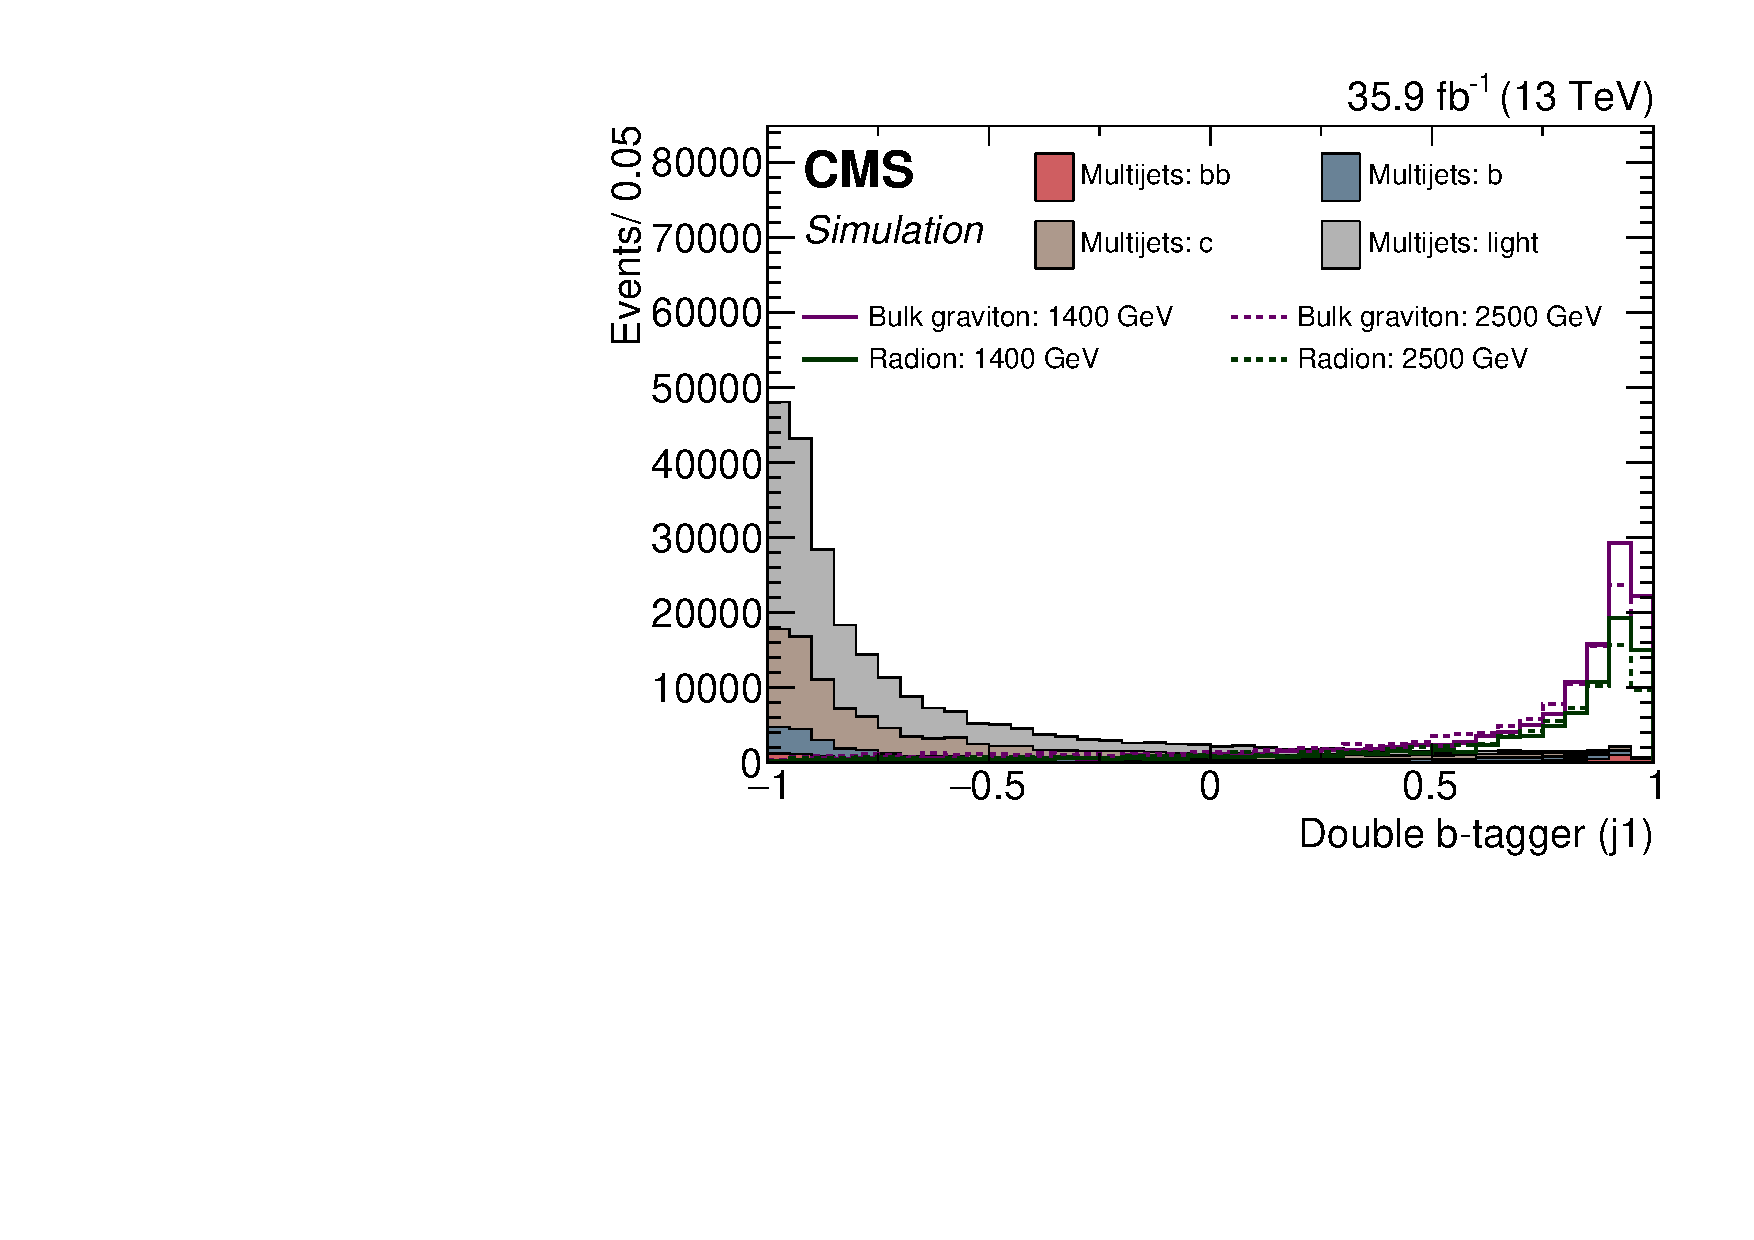
\includegraphics[width=0.45\textwidth]{Analysis/EventSelection/cmc_doubleSV_j0.pdf}
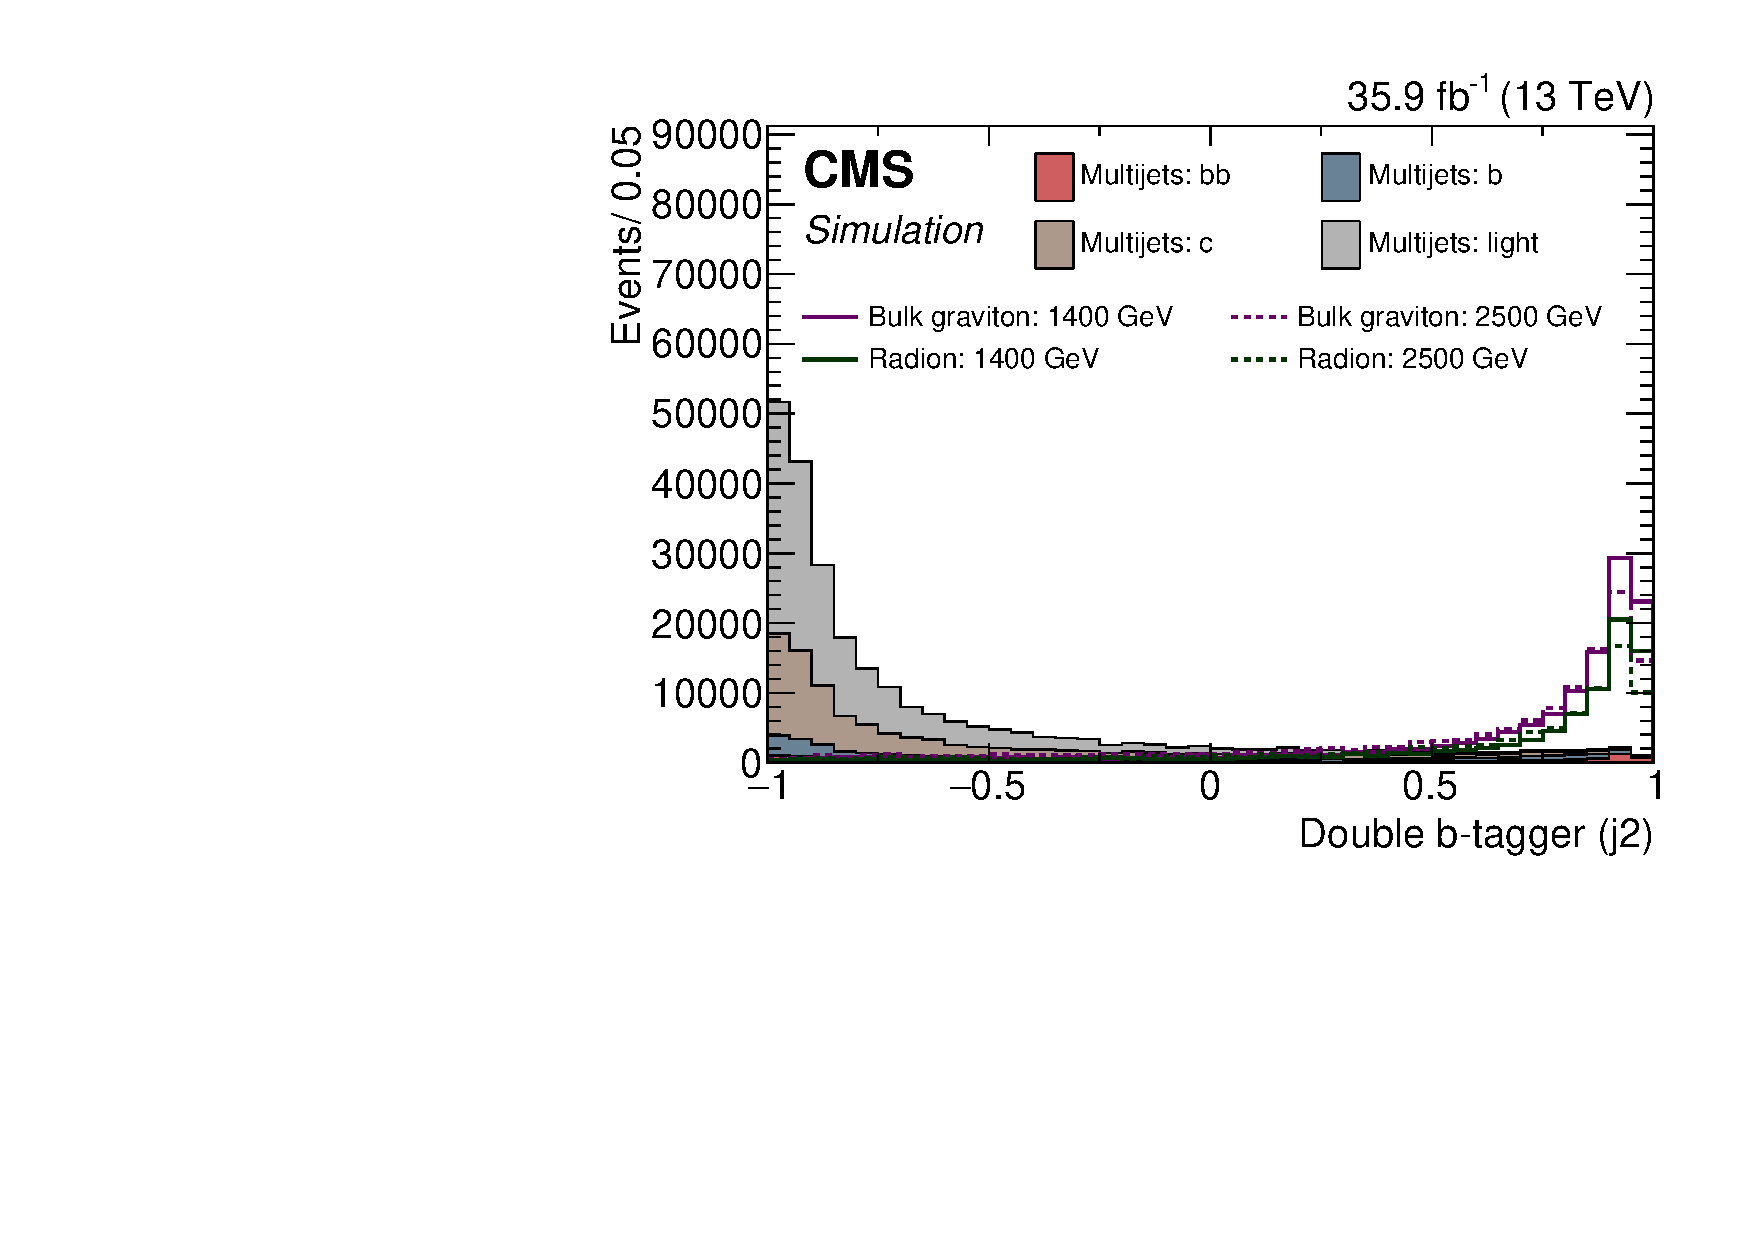
\includegraphics[width=0.45\textwidth]{Analysis/EventSelection/cmc_doubleSV_j1.pdf}
\caption{ Comparison of simulated events after all pre-selection criteria, for the double b-tagger discriminant
  of the leading (left) and sub-leading (right) Higgs-jets. A signal cross section of 20~pb is assumed for each signal mass point.
\label{fig:doublesv_prebtag}
}
\end{figure}

The cut flow for the full event selection outlined in the previous section is given in Table~\ref{tab:BulkGravCutFlowEff} for bulk gravitons and in Table~\ref{tab:RadionCutFlowEff} for radions. The main difference in the efficiencies of the spin-2 and the spin-0 models stems from the different $\Delta\eta_{jj}$ distributions, that for the bulk graviton being more central. Therefore, the bulk gravitions have a higher efficiency than the radions.

\begin{table}[h]
\begin{center}
\scalebox{0.65}{
\begin{tabular}{|l|c|c|c|c|c|c|c|c|c|c|}
\hline
Mass (GeV) & $\ge 2$ AK8 jets + triggers & jet $p_{T}$, $\eta$ & Tight jet ID & $\Delta\eta_{jj}$ & Lepton Veto & $\tau_{21}$ & jet mass & $M_{jj}^{red}$ & double-b tag $>0.3$ & double-b tag $>0.8$ \\ \hline
750 & 0.610 & 0.368 & 0.368 & 0.331 & 0.330 & 0.149 & 0.049 & 0.039 & 0.027 & 0.015 \\
800 & 0.758 & 0.541 & 0.541 & 0.503 & 0.502 & 0.237 & 0.080 & 0.079 & 0.057 & 0.032 \\
900 & 0.903 & 0.772 & 0.771 & 0.716 & 0.715 & 0.371 & 0.125 & 0.124 & 0.092 & 0.051 \\
1000 & 0.958 & 0.885 & 0.885 & 0.801 & 0.799 & 0.434 & 0.151 & 0.151 & 0.111 & 0.062 \\
1200 & 0.988 & 0.962 & 0.961 & 0.843 & 0.842 & 0.499 & 0.178 & 0.178 & 0.129 & 0.068 \\
1400 & 0.996 & 0.984 & 0.983 & 0.854 & 0.853 & 0.524 & 0.182 & 0.182 & 0.129 & 0.064 \\
1600 & 0.998 & 0.993 & 0.993 & 0.858 & 0.857 & 0.532 & 0.186 & 0.186 & 0.128 & 0.061 \\
1800 & 0.999 & 0.996 & 0.996 & 0.864 & 0.863 & 0.543 & 0.193 & 0.193 & 0.130 & 0.059 \\
2000 & 1.000 & 0.998 & 0.998 & 0.861 & 0.860 & 0.541 & 0.190 & 0.190 & 0.123 & 0.054 \\
2500 & 1.000 & 0.999 & 0.999 & 0.862 & 0.862 & 0.538 & 0.188 & 0.188 & 0.113 & 0.044 \\
3000 & 1.000 & 1.000 & 0.999 & 0.865 & 0.865 & 0.530 & 0.186 & 0.186 & 0.102 & 0.034 \\
4000 & 1.000 & 1.000 & 0.999 & 0.861 & 0.861 & 0.505 & 0.166 & 0.166 & 0.078 & 0.021 \\
4500 & 1.000 & 1.000 & 0.999 & 0.859 & 0.858 & 0.502 & 0.156 & 0.156 & 0.065 & 0.016 \\
\hline
\end{tabular}
}
\caption{ Efficiencies for event selection for spin-2 bulk gravitons. The selections applied are $\tau_{21} < 0.55$,  $105 < m_{soft-drop} < 135$ and for all the three operating points for the double-b tagger\label{tab:BulkGravCutFlowEff}}.
\end{center}
\end{table}

\begin{table}[h]
\begin{center}
\scalebox{0.65}{
\begin{tabular}{|l|c|c|c|c|c|c|c|c|c|c|}
\hline
Mass (GeV) & $\ge 2$ AK8 jets + triggers & jet $p_{T}$, $\eta$ & Tight jet ID & $\Delta\eta_{jj}$ & Lepton Veto & $\tau_{21}$ & jet mass & $M_{jj}^{red}$ & double-b tag $>0.3$ & double-b tag $>0.8$ \\ \hline
750 & 0.432 & 0.248 & 0.247 & 0.213 & 0.213 & 0.093 & 0.029 & 0.024 & 0.016 & 0.009 \\
800 & 0.547 & 0.367 & 0.367 & 0.327 & 0.326 & 0.152 & 0.051 & 0.050 & 0.036 & 0.021 \\
900 & 0.693 & 0.552 & 0.552 & 0.487 & 0.485 & 0.245 & 0.083 & 0.083 & 0.061 & 0.033 \\
1000 & 0.772 & 0.666 & 0.666 & 0.552 & 0.550 & 0.296 & 0.101 & 0.101 & 0.075 & 0.041 \\
1200 & 0.859 & 0.792 & 0.792 & 0.585 & 0.584 & 0.335 & 0.116 & 0.116 & 0.084 & 0.044 \\
1400 & 0.902 & 0.854 & 0.854 & 0.591 & 0.590 & 0.355 & 0.123 & 0.123 & 0.087 & 0.044 \\
1600 & 0.928 & 0.890 & 0.889 & 0.592 & 0.591 & 0.358 & 0.124 & 0.124 & 0.086 & 0.041 \\
1800 & 0.946 & 0.913 & 0.913 & 0.595 & 0.594 & 0.365 & 0.124 & 0.124 & 0.082 & 0.036 \\
2000 & 0.957 & 0.931 & 0.931 & 0.598 & 0.598 & 0.365 & 0.127 & 0.127 & 0.081 & 0.036 \\
2500 & 0.975 & 0.956 & 0.955 & 0.596 & 0.595 & 0.367 & 0.125 & 0.125 & 0.076 & 0.030 \\
3000 & 0.981 & 0.966 & 0.965 & 0.589 & 0.589 & 0.357 & 0.123 & 0.123 & 0.068 & 0.022 \\
3500 & 0.987 & 0.973 & 0.972 & 0.582 & 0.582 & 0.349 & 0.116 & 0.116 & 0.059 & 0.018 \\
4500 & 0.991 & 0.977 & 0.976 & 0.579 & 0.578 & 0.334 & 0.103 & 0.103 & 0.044 & 0.010 \\
\hline
\end{tabular}
}
\caption{ Efficiencies for event selection for spin-0 radions. The selections applied are $\tau_{21} < 0.55$,  $105 < m_{soft-drop} < 135$ and for all the three operating points for the double-b tagger\label{tab:RadionCutFlowEff}}.
\end{center}
\end{table}

In order to study the background composition of the events passing our selection criteria and the data to MC agreement without unblinding, two different control regions have been defined. These regions are built by inverting either the $\tau_{21}$ or the double-b tag cuts for exactly one of the two selected jets.

\noindent
\textbf{N-subjettiness inverted control region}:
The $\tau_{21}$ inverted control region has been selected by applying all of the event selection criteria except the $\tau_{21}$ requirement on the leading jet. Instead this jet is required to fail $tau_{21}$ requirement.
In this comparison no SF is applied and simulation yield is scaled to match the one in data (data/MC is $\approx 1.26$) in Figures \ref{fig:jet1_tau_inverted} and \ref{fig:jet2_tau_inverted}.
The major background from QCD multijet production is simulated and compared with the data. The multijet background has been split by flavor content.

\begin{figure}[H]
\centering
\includegraphics[width=0.45\textwidth]{Analysis/EventSelection/anti_tau21_rereco_doublebtagv4/puppiSDMassThea_j0.pdf}
\includegraphics[width=0.45\textwidth]{Analysis/EventSelection/anti_tau21_rereco_doublebtagv4/pt_j0.pdf}
\includegraphics[width=0.45\textwidth]{Analysis/EventSelection/anti_tau21_rereco_doublebtagv4/eta_j0.pdf}
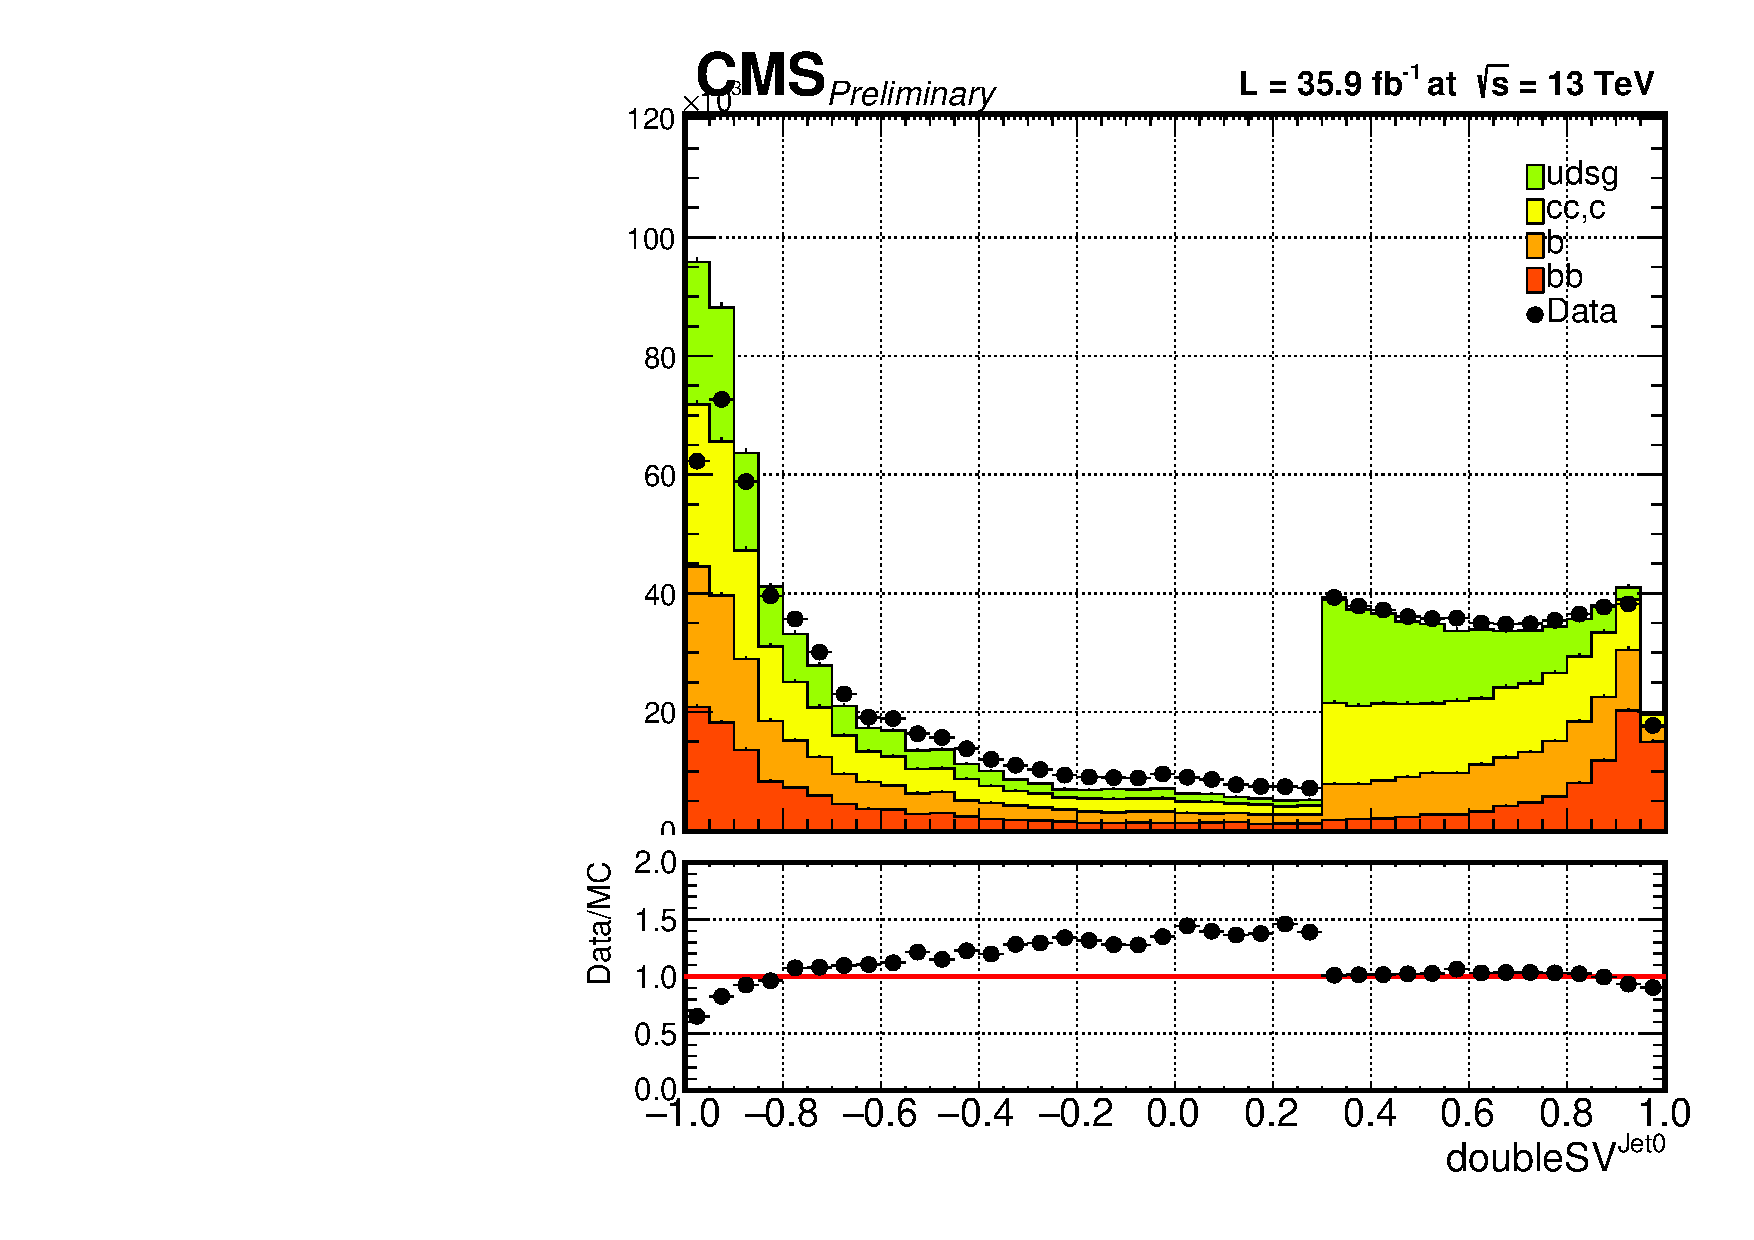
\includegraphics[width=0.45\textwidth]{Analysis/EventSelection/anti_tau21_rereco_doublebtagv4/doubleSV_j0.pdf}
\caption{ Comparison plots of data/simulation for kinematic observables and double-b tag value for the leading jet in the $\tau_{21}$ inverted control sample. From left to right: Thea-corrected softdrop mass, $p_{T}$, $\eta$ and double-b tag discriminator.}
\label{fig:jet1_tau_inverted}
\end{figure}

\begin{figure}[H]
\centering
\includegraphics[width=0.45\textwidth]{Analysis/EventSelection/anti_tau21_rereco_doublebtagv4/puppiSDMassThea_j1.pdf}
\includegraphics[width=0.45\textwidth]{Analysis/EventSelection/anti_tau21_rereco_doublebtagv4/pt_j1.pdf}
\includegraphics[width=0.45\textwidth]{Analysis/EventSelection/anti_tau21_rereco_doublebtagv4/eta_j1.pdf}
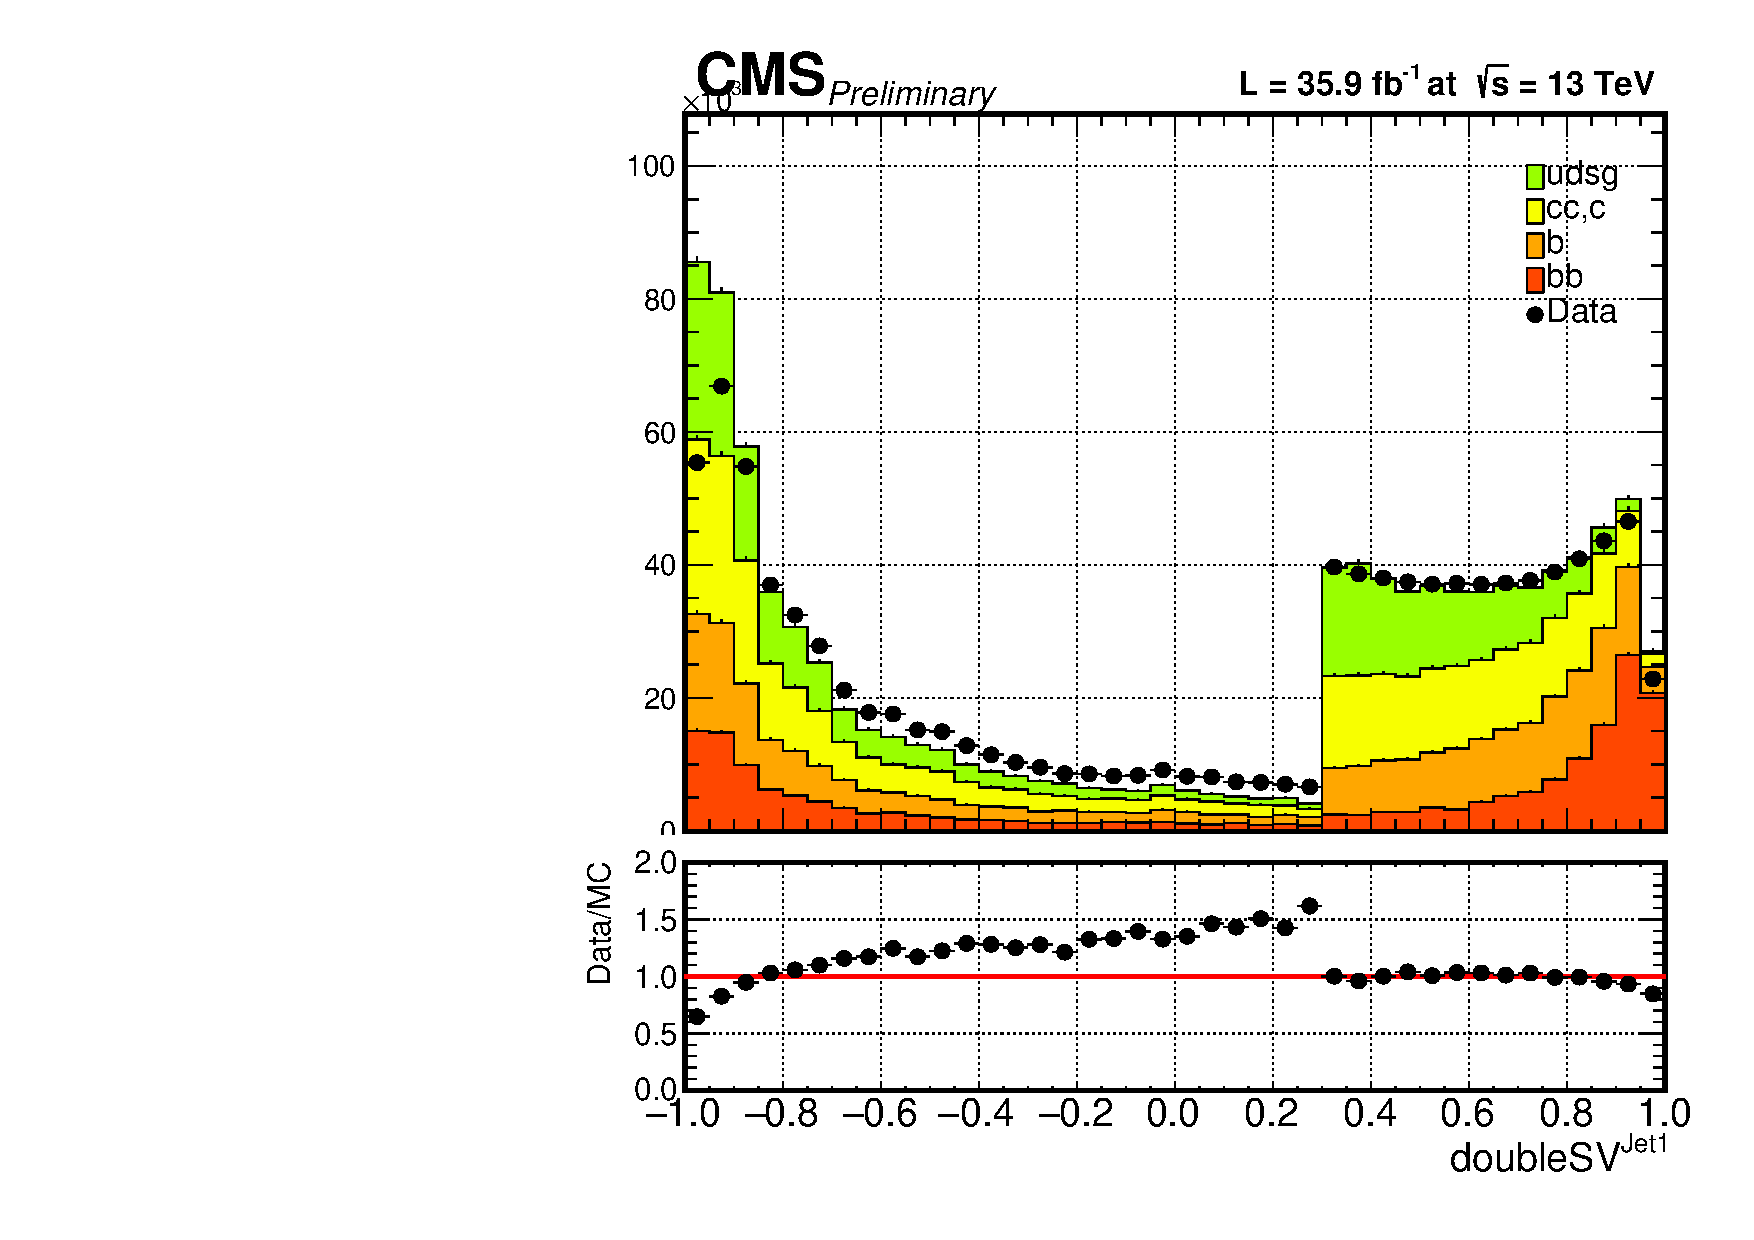
\includegraphics[width=0.45\textwidth]{Analysis/EventSelection/anti_tau21_rereco_doublebtagv4/doubleSV_j1.pdf}
\caption{ Comparison plots of data/simulation for kinematic observables and double-b tag value for the second jet in the $\tau_{21}$ inverted control sample. From left to right: Thea-corrected softdrop mass, $p_{T}$, $\eta$ and double-b tag discriminator.}
\label{fig:jet2_tau_inverted}
\end{figure}


\begin{figure}[H]
\centering
\includegraphics[width=0.9\textwidth]{Analysis/EventSelection/anti_tau21_rereco_doublebtagv4/deltaEta.pdf}
\caption{ Comparison plot of data/simulation for the pseudorapidity difference between the two Higgs-jet candidates $\Delta\eta_{jj}$ in the $\tau_{21}$ inverted control sample.}
\label{fig:deta_tau_inverted}
\end{figure}

\noindent
\textbf{Double-b inverted control region}:
The double-b tag inverted control region has been selected by applying all the event selection criteria except for the double-b tag requirement on the leading jet. Instead the leading jet is required to fail the double-b tag loose requirement.
In this comparison no SF is applied and simulation yield is scaled to match the one in data (Data/MC is $\approx 0.88$) in Figures \ref{fig:jet1_double-b_tag_inverted} and \ref{fig:jet2_double-b_tag_inverted}. The main contributing background is multi-jet production from QCD.

\begin{figure}[H]
\centering
\includegraphics[width=0.45\textwidth]{Analysis/EventSelection/anti_doublebtag_rereco_doublebtagv4/puppiSDMassThea_j0.pdf}
\includegraphics[width=0.45\textwidth]{Analysis/EventSelection/anti_doublebtag_rereco_doublebtagv4/pt_j0.pdf}
\includegraphics[width=0.45\textwidth]{Analysis/EventSelection/anti_doublebtag_rereco_doublebtagv4/eta_j0.pdf}
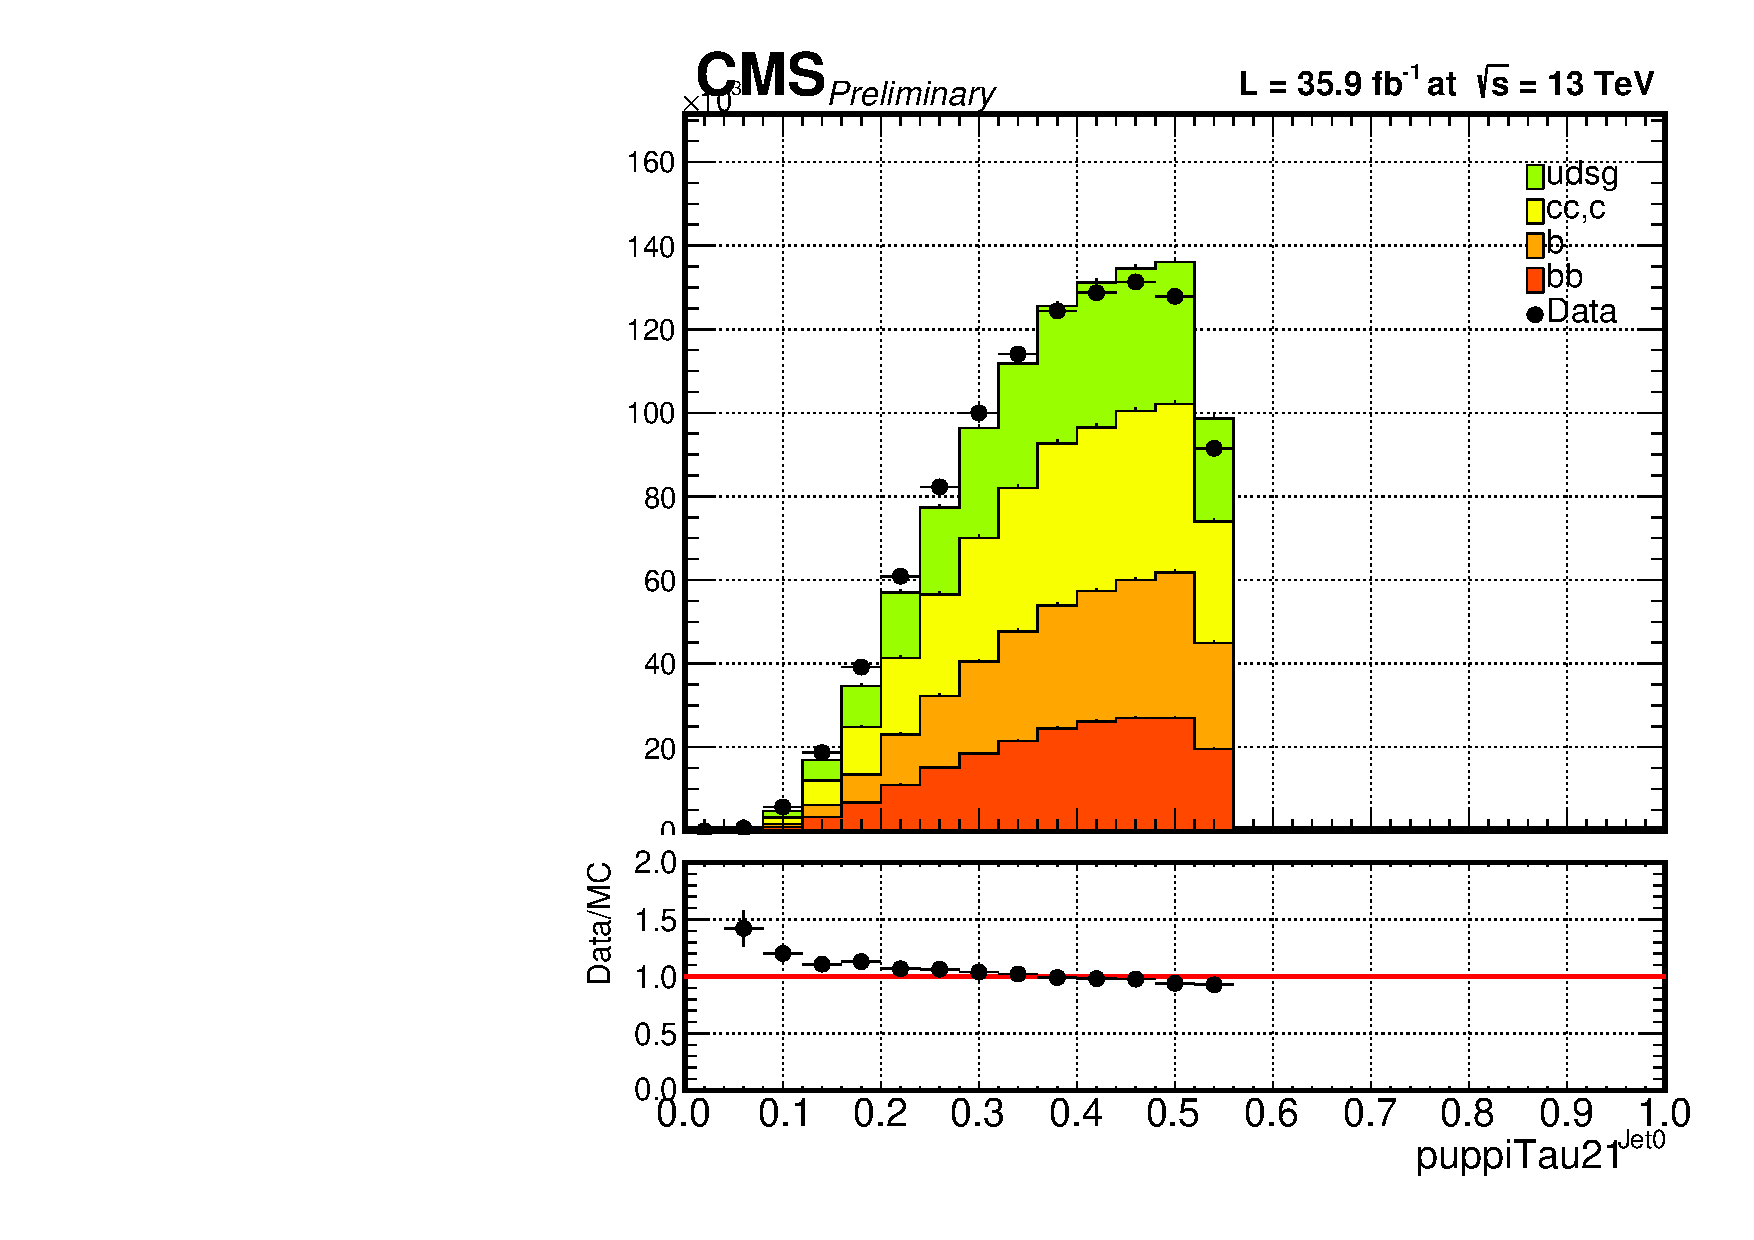
\includegraphics[width=0.45\textwidth]{Analysis/EventSelection/anti_doublebtag_rereco_doublebtagv4/puppiTau21_j0.pdf}
\caption{ Comparison plots of data/simulation for kinematic and substructure observables for the leading jet in the double-b tag inverted control sample. From left to right: Thea-corrected softdrop mass, $p_{T}$, $\eta$ and $\tau_{21}$.}
\label{fig:jet1_double-b_tag_inverted}
\end{figure}

\begin{figure}[H]
\centering
\includegraphics[width=0.45\textwidth]{Analysis/EventSelection/anti_doublebtag_rereco_doublebtagv4/puppiSDMassThea_j1.pdf}
\includegraphics[width=0.45\textwidth]{Analysis/EventSelection/anti_doublebtag_rereco_doublebtagv4/pt_j1.pdf}
\includegraphics[width=0.45\textwidth]{Analysis/EventSelection/anti_doublebtag_rereco_doublebtagv4/eta_j1.pdf}
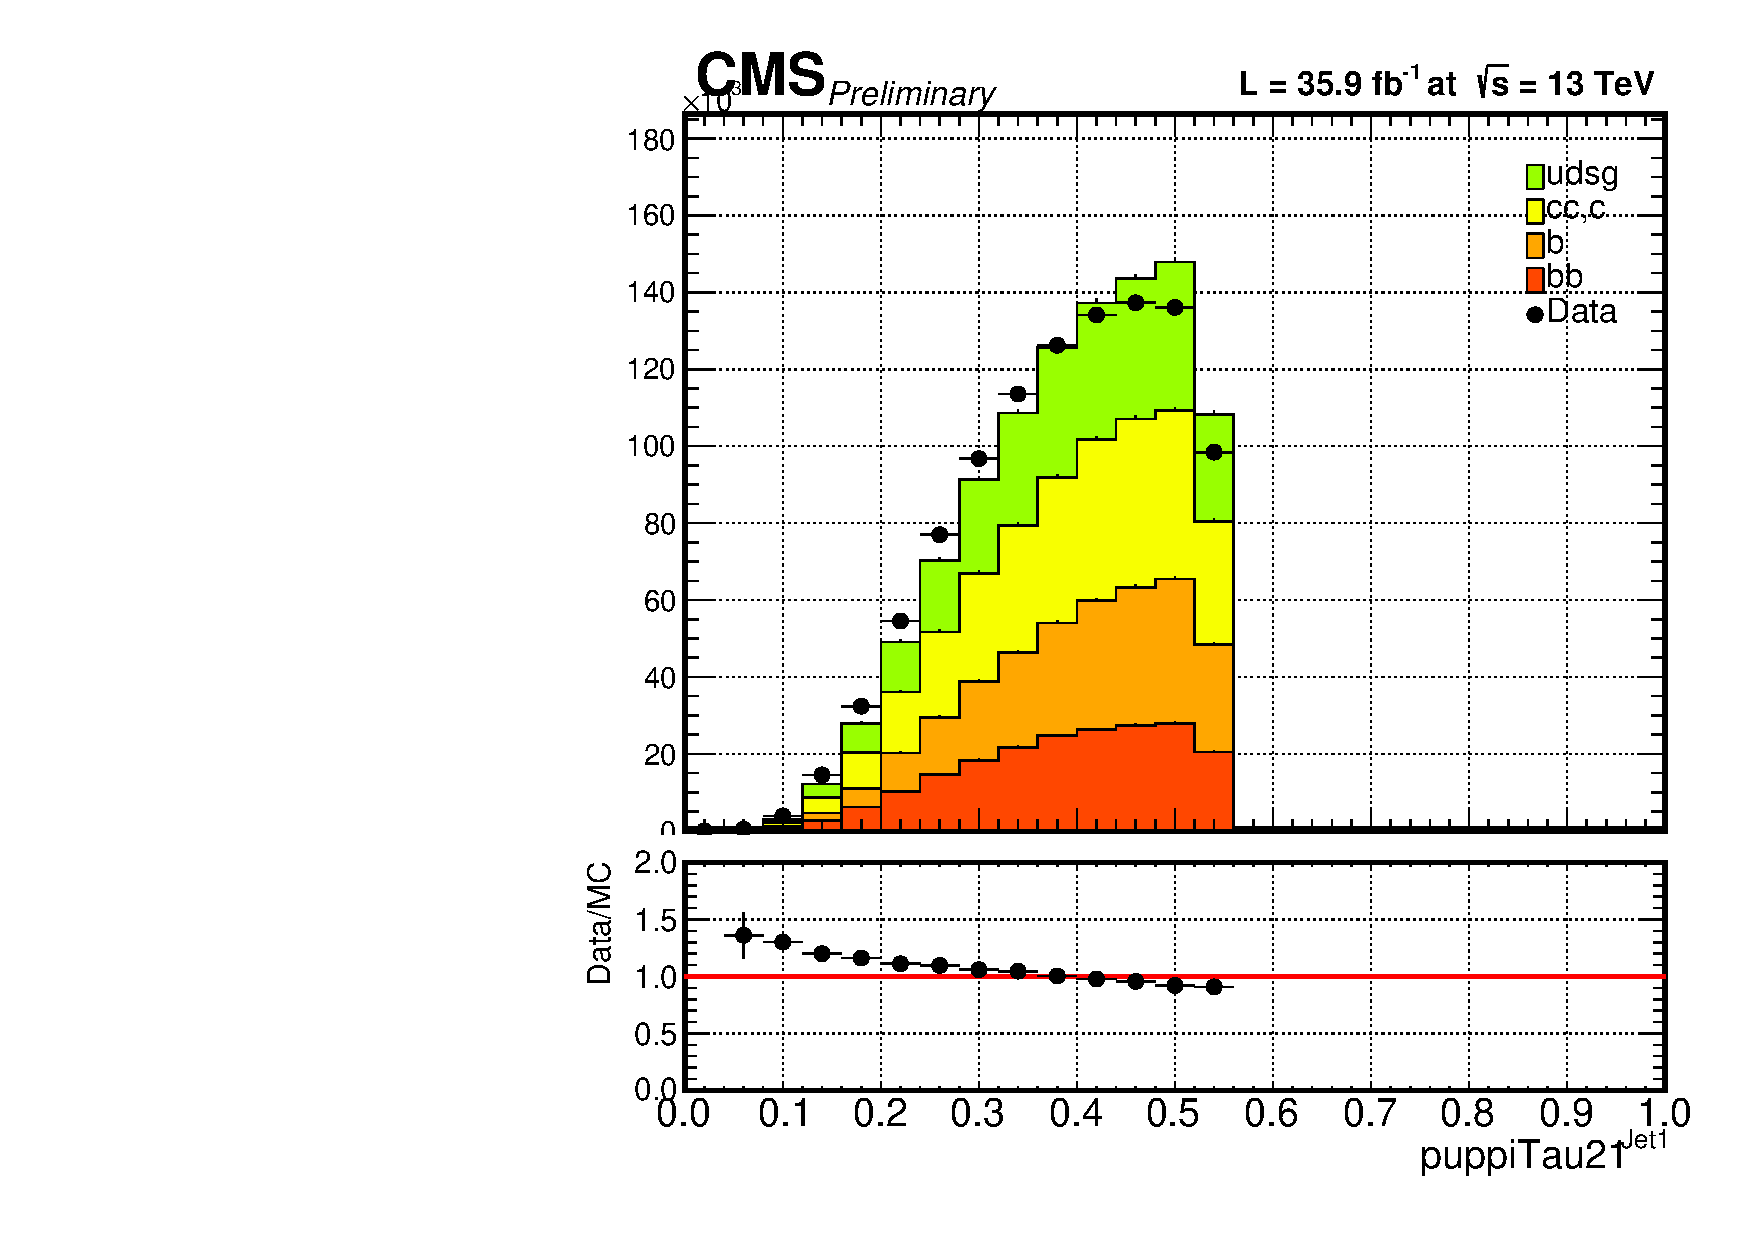
\includegraphics[width=0.45\textwidth]{Analysis/EventSelection/anti_doublebtag_rereco_doublebtagv4/puppiTau21_j1.pdf}
\caption{ Comparison plots of data/simulation for kinematic and substructure observables for the second jet in the double-b tag inverted control sample. From left to right: Thea-corrected softdrop mass, $p_{T}$, $\eta$ and $\tau_{21}$.}
\label{fig:jet2_double-b_tag_inverted}
\end{figure}

\begin{figure}[H]
\centering
\includegraphics[width=0.9\textwidth]{Analysis/EventSelection/anti_doublebtag_rereco_doublebtagv4/deltaEta.pdf}
\caption{ Comparison plot of data/simulation for the pseudorapidity difference between the two Higgs-jet candidates $\Delta\eta_{jj}$ in the double-b tag inverted control sample.}
\label{fig:deta_double-b_tag_inverted}
\end{figure}

\section{Background Estimation}
\label{sec:BkgEst}

Two different background modelling techniques are used depending on whether the $M_{jj}^{red}$ region is above or below the trigger turnon. Above the trigger turnon, $M_{jj}^{red} \ge 1200$ GeV, the background is smoothly falling and therefore the shape can be modeled by a smooth function and the "Alphabet Assisted Bump Hunt" method is used. Below the trigger turnon, $M_{jj}^{red} < 1200$ GeV, the inefficiency in the trigger causes the background to not fall smoothly and therefore an estimation is made by reweighting every event in a control region with a technique called the "Alphabet" method.

Both of these techniques are data-driven methods which exploit a number of sidebands. These sidebands are defined with respect to the leading $p_{T}$ jet based on its softdrop mass and the value of the double-b discriminant. Using these two variables, a set of regions is defined as outlined in Figure~\ref{fig:ABCDEFregions}. All of these regions together, defined as the pre-tag region, are populated by events that pass all selection requirements except for the soft-drop mass and double-b tagger requirements on the leading jet. The signal region is the subset of those events which pass the soft-drop mass and double-b requirements on the leading jet. The anti-tag region is the subset of pre-tag events which pass the soft-drop mass requirement but fail the double-b requirement on the leading jet. All other events in the pre-tag region constitute the mass sidebands. 

\begin{figure}[H]
  \centering
    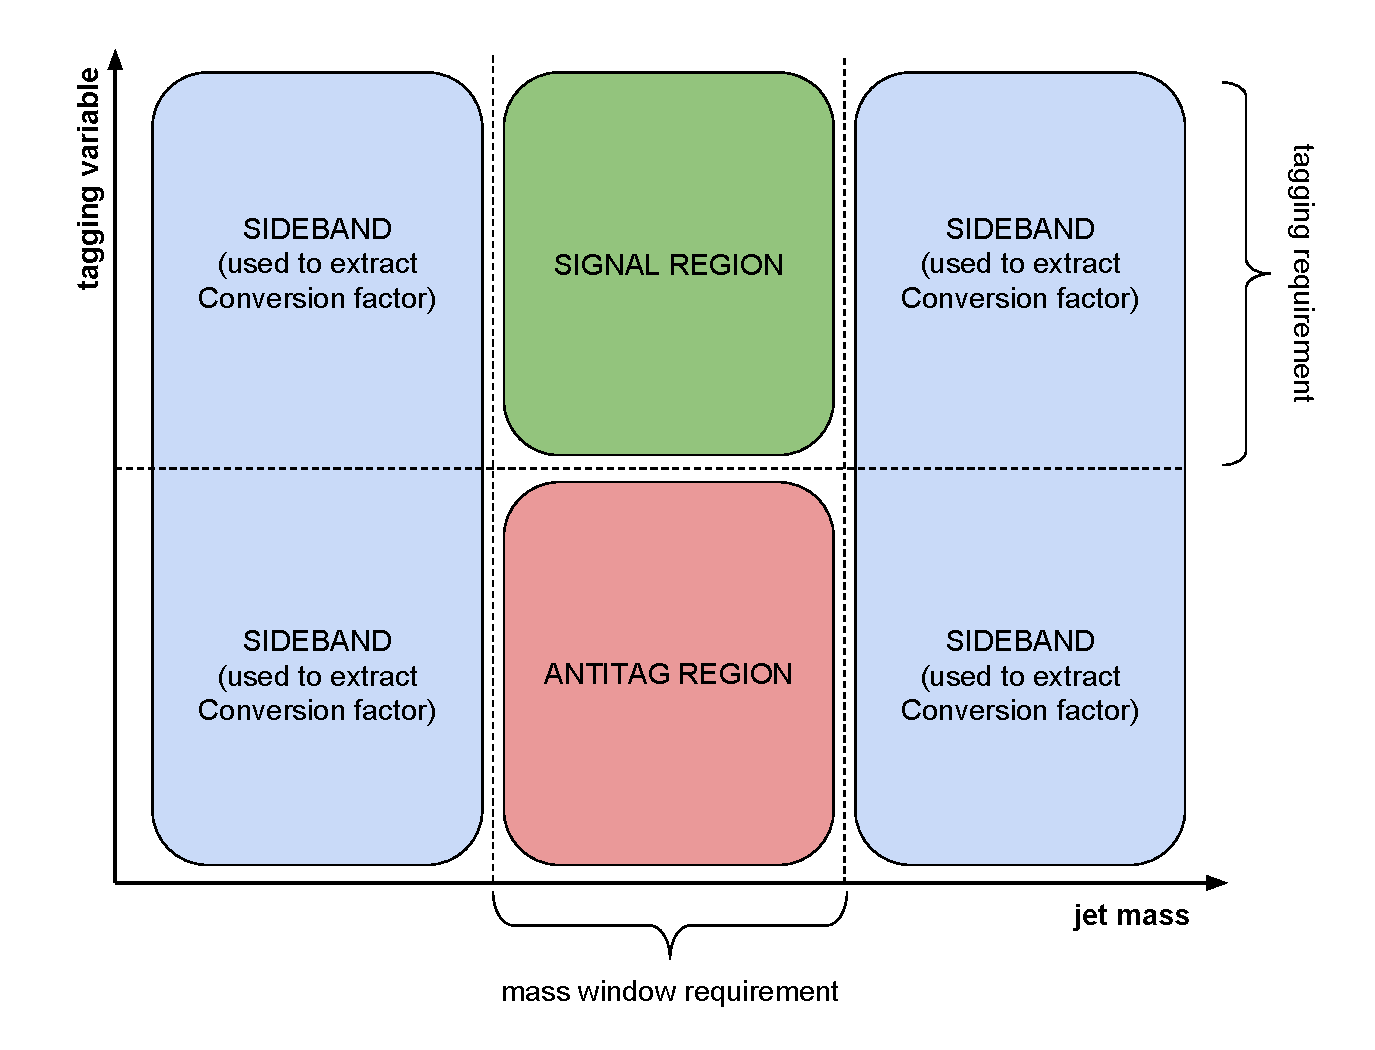
\includegraphics[width=\textwidth]{Analysis/BackgroundEstimation/pretag2.pdf}
  \caption{Schematic representation of the regions used to perform the background estimate.} \label{fig:ABCDEFregions}
\end{figure}

\subsection{Alphabet Method}

The Alphabet method is an extension of a common background estimation technique called the "ABCD" method. Both of these methods expect the shapes but not the normalizations of distributions of events in the signal and anti-tag regions to be the same. If there was no correlation between the soft-drop mass and the double-b tagger, the ABCD method could be used. This method only uses a single sideband to measure the ratio of passing to failing events and then scales the anti-tag region by this ratio to obtain an estimate of the signal region. As can be seen in Figure~\ref{fig:twotone2}, where the full preselection has been applied to simulated events, the double-b discriminator has a slight dependence on the soft-drop mass. Therefore, to obtain the normalization, a conversion ratio or the pass-faill ratio, $R_{p/f}$, that depends on the leading jet mass is extracted from the multiple jet mass sidebands. This is done by fitting a quadratic function to the variation of $R_{p/f}$ as a function of the leading jet mass. An alternative fit using a third order polynomial was found to give the same interpolated value of $R_{p/f}$ in the Higgs jet mass window. Every event in the antitag region is scaled by the pass-fail evaluated for the leading jet mass of that event, to obtain the background prediction in the signal region. 

\begin{figure}[H]
  \centering
    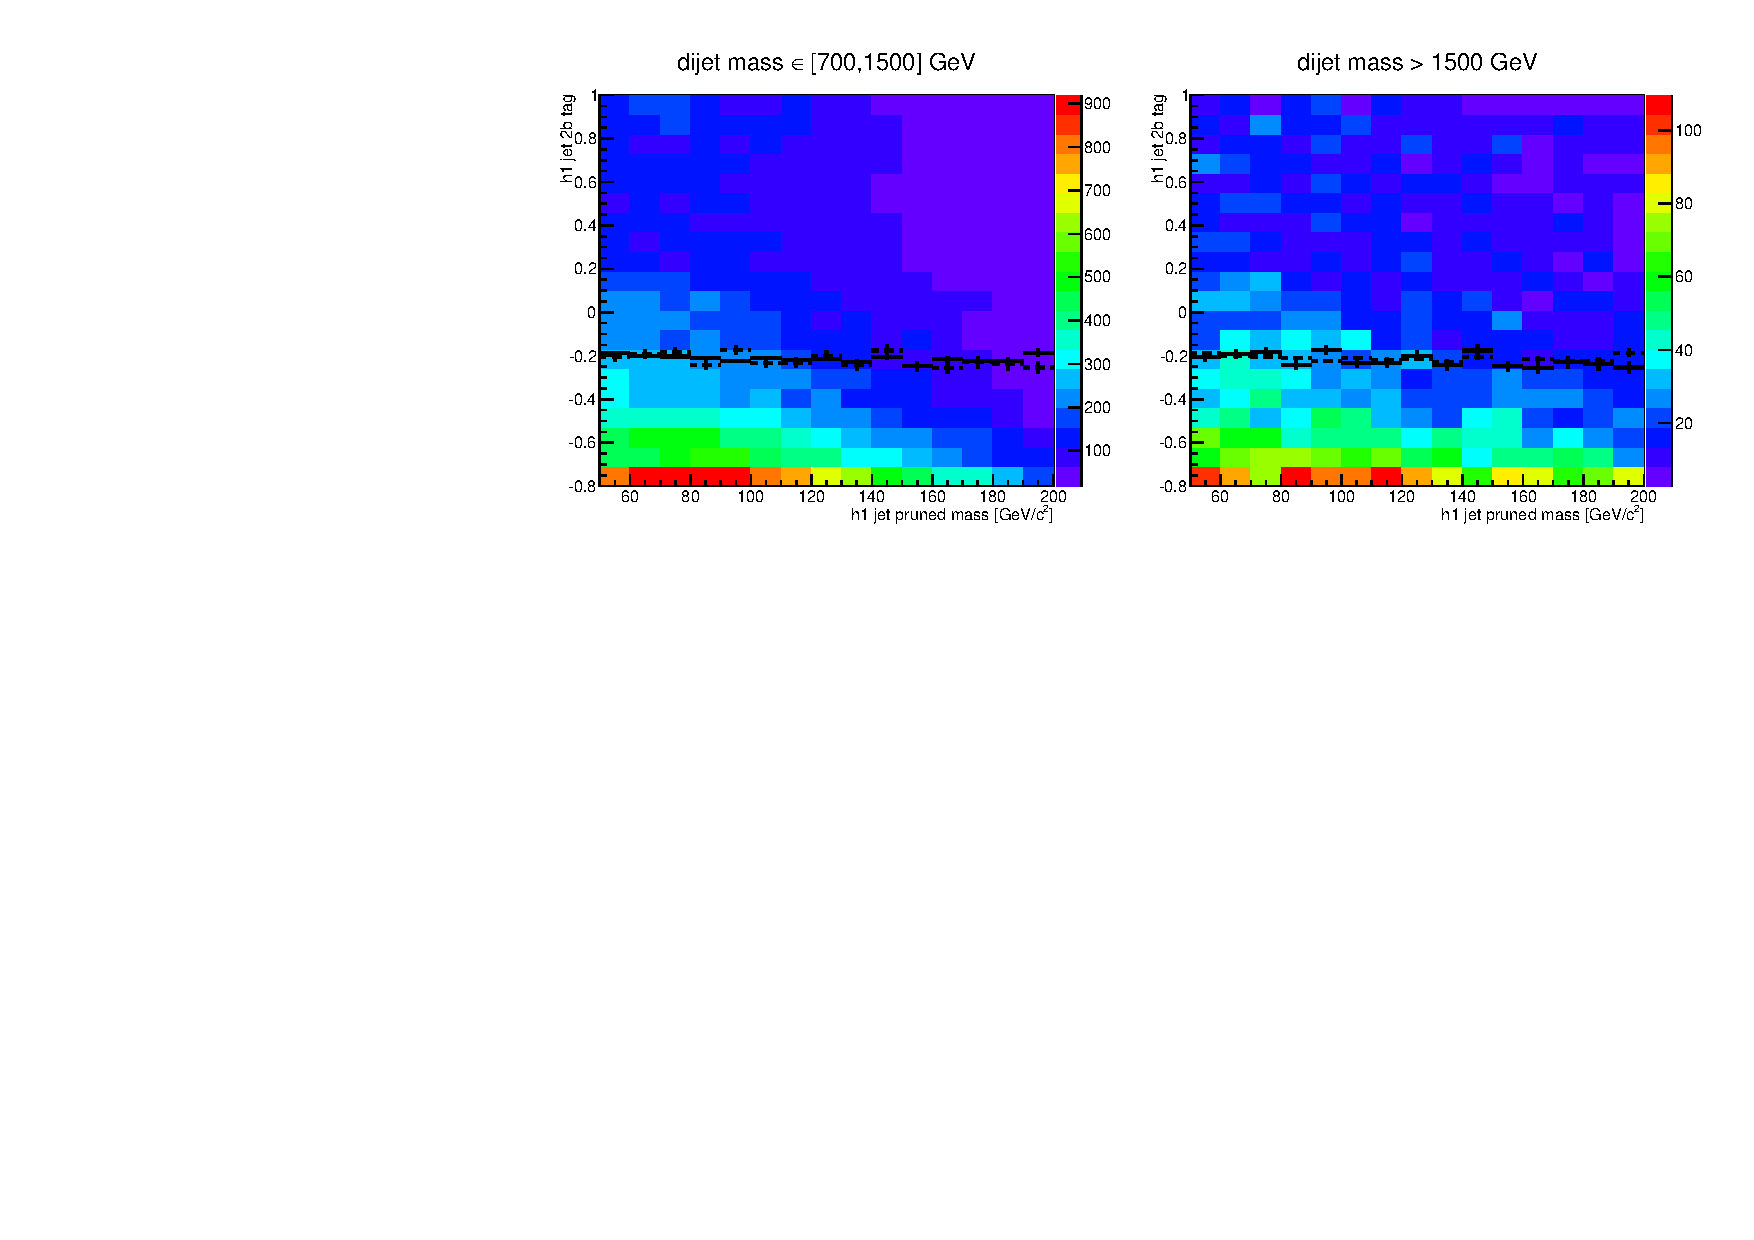
\includegraphics[width=\textwidth]{Analysis/BackgroundEstimation/TwoToneBAfter.pdf}
  \caption{Dependence of the double b-tagger on the jet mass after the preselection is applied. We separate high HT and low HT events. The solid curve represents the profile distribution of a respective region while the dashed line is the profile of the other HT region.} \label{fig:twotone2}
\end{figure}

\subsubsection{Results in Simulation}

Prior to unblinding the data, the validity of the Alphabet method needed to be tested. This was first done by using the Alphabet method on simulation. Figure \ref{F:closuresim} (left) shows a quadratic fit in the mass sidebands of the conversion rate $R_{p/f}$ to pass the requirement double-b$ > 0.6$, in QCD MC for the full selection. Note that the signal region and anti-tag regions are not included in the fit. The true value of the conversion rate in this mass window is also shown in the figure. This conversion rate is then applied (as a function of mass) to the anti-tag region to obtain an estimate of the signal region. The estimated and true background in signal region are shown in Figure \ref{F:closuresim} (right).Two systematic uncertainties arise naturally from this estimate. The dominant error is the uncertainty in the fit to the mass sideband regions. The uncertainty in the fit is shown as a dashed line enveloping the fit in Figure \ref{F:closuresim} (left). This error can be treated as fully correlated between all mass bins when setting limits. The second source of error comes from propagating the statistical uncertainty in the anti-tag region to the signal region. This error is uncorrelated between bins and is smaller than the fitting error. Both errors are shown in the figure.

\begin{figure}[H]
\centering
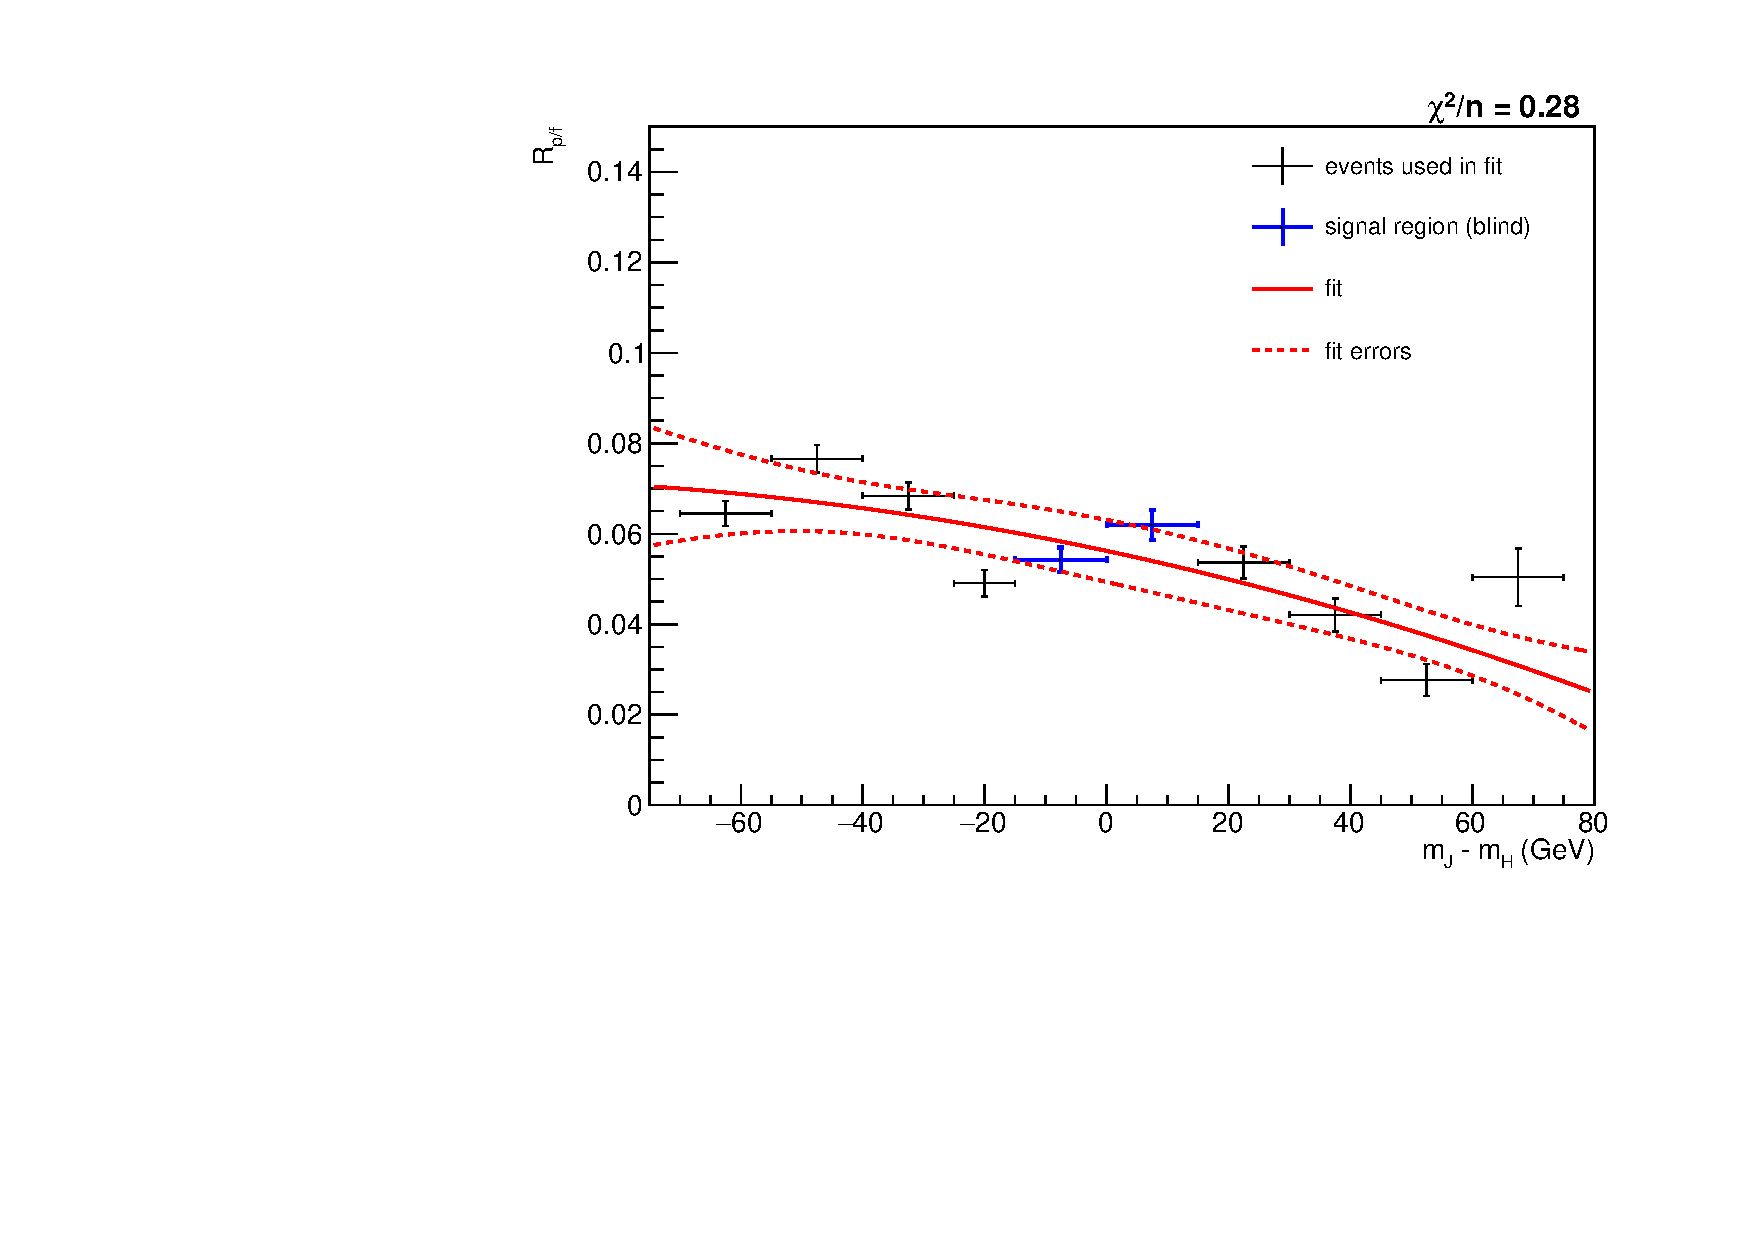
\includegraphics[width=0.45\textwidth]{Analysis/BackgroundEstimation/HHSR_Fit_HH_MM_QCD.pdf}
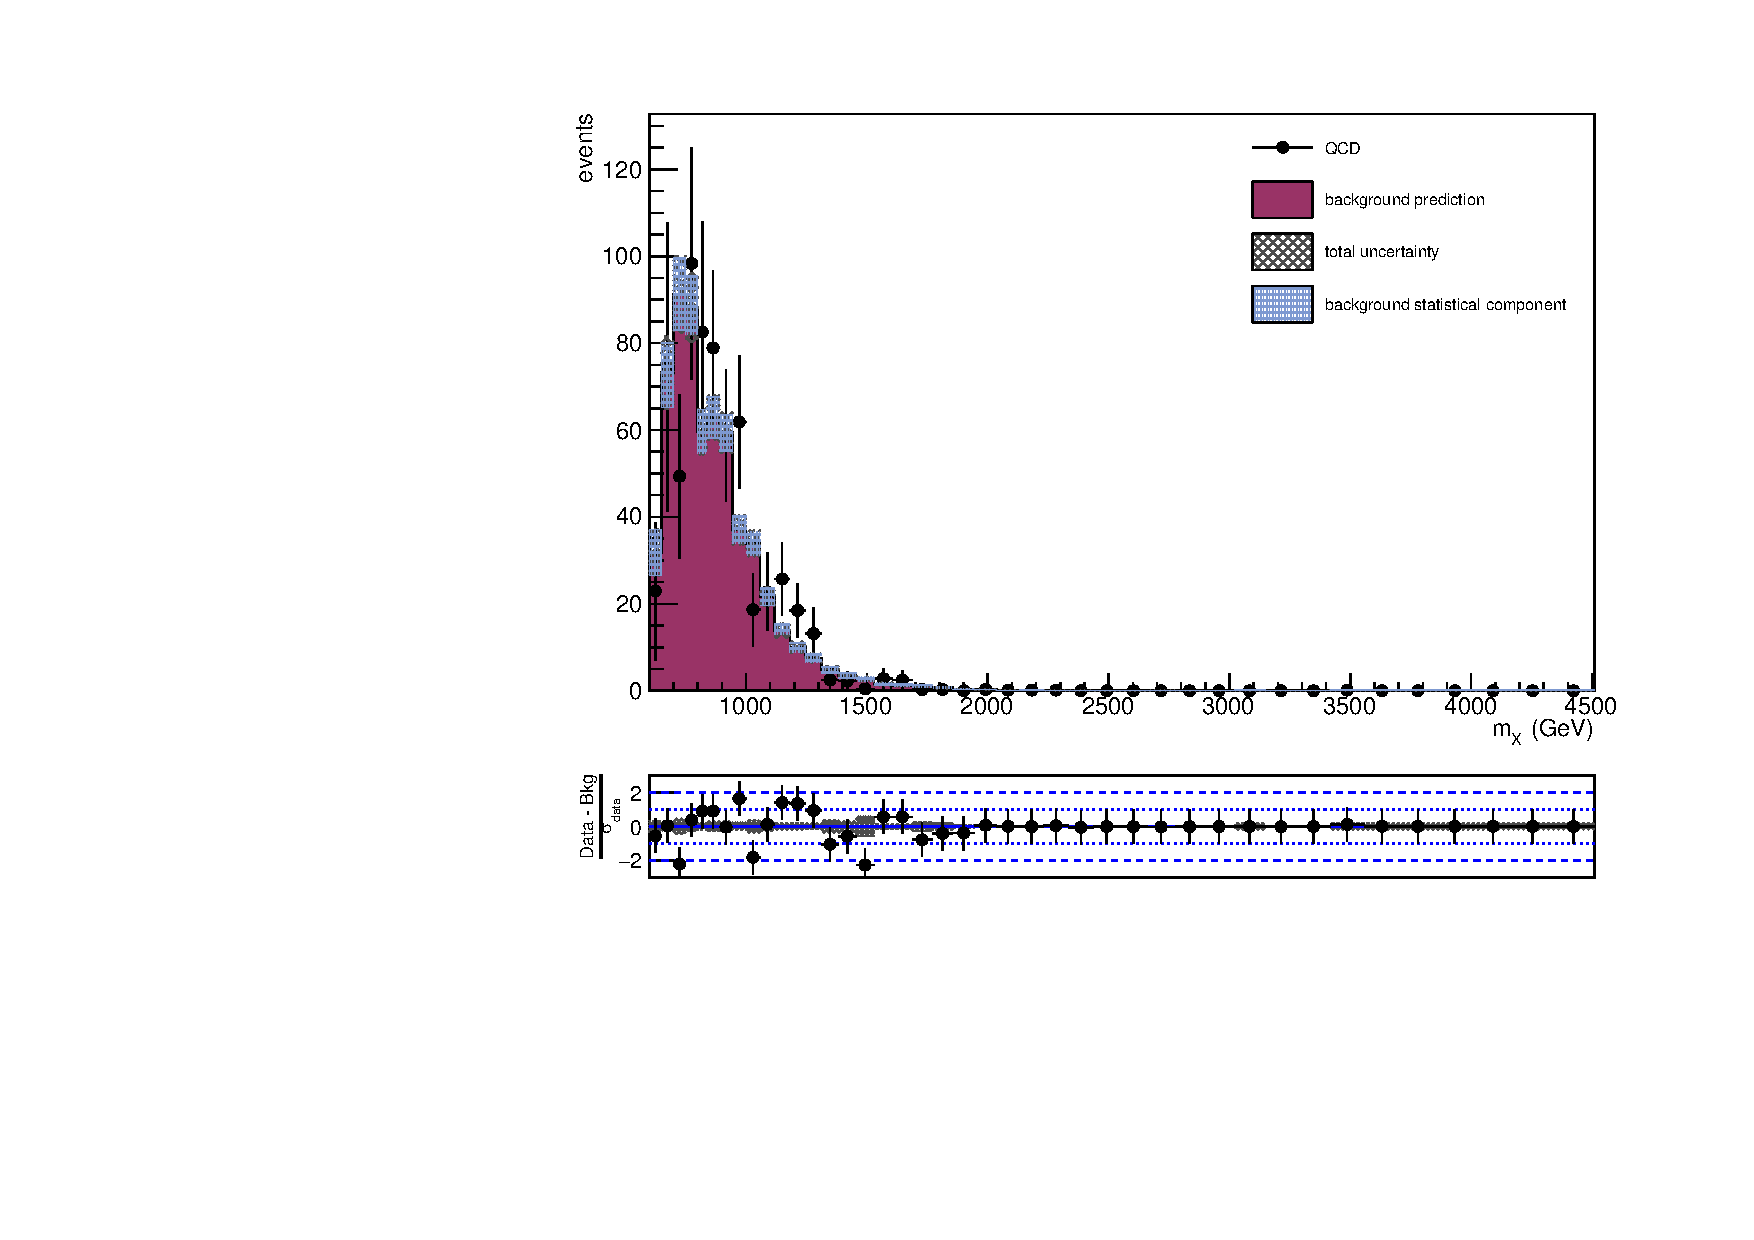
\includegraphics[width=0.45\textwidth]{Analysis/BackgroundEstimation/HHSR_Plot_SigTestQCD.pdf}\\
  \caption{For QCD simulation: (left) Fit in the mass sideband regions for the conversion rate $R_{p/f}$ and (right) application of that fit to the anti-tag region to estimate the background in the signal region, both jets pass the medium double-b tagger working point ($> 0.6$), compared with the true background (black markers).}
\label{F:closuresim}
\end{figure}

\subsubsection{Closure Test in Data}

As a further test of closure, we test our method in data, estimating the QCD content of a region similar to the signal region except that the 2$^{nd}$ jet is constrained to fail the double-b requirement. Results are shown in Figure \ref{F:closuredata} in the same format as for the closure test in QCD, for three values of the cut on the double-b: 0.8 (tight), 0.6 (medium) and 0.3 (loose).

\begin{figure}[H]
\centering
\includegraphics[width=0.45\textwidth]{Analysis/BackgroundEstimation/HHSR_Fit_T0.pdf}
\includegraphics[width=0.45\textwidth]{Analysis/BackgroundEstimation/HHSR_Plot_T0.pdf}
\includegraphics[width=0.45\textwidth]{Analysis/BackgroundEstimation/HHSR_Fit_M0.pdf}
\includegraphics[width=0.45\textwidth]{Analysis/BackgroundEstimation/HHSR_Plot_M0.pdf}
\includegraphics[width=0.45\textwidth]{Analysis/BackgroundEstimation/HHSR_Fit_L0.pdf}
\includegraphics[width=0.45\textwidth]{Analysis/BackgroundEstimation/HHSR_Plot_L0.pdf}
\caption{(left) Fits in the mass sideband regions for the conversion rates $R_{p/f}$ for (from top to bottom) the Tight, Medium and Loose working point.(right) Application of those fits to the anti-tag region to estimate the background in the control regions, compared with the true background (black markers).}
\label{F:closuredata}
\end{figure}

To further test this method, a check was performed to verify that the estimate is free of bias when a signal is introduced. This was done by injecting a bulk graviton signal sample with bulk graviton mass at 1800 GeV and the cross section scaled to $0.1$ fb into the QCD MC. The Alphabet method was then performed and the results can be seen in Figure~\ref{fig:INJ}. The background estimate performs well, with the addition of this signal having no significant effect on the background estimate.

\begin{figure}[H]
  \centering
    \includegraphics[width=0.45\textwidth]{Analysis/BackgroundEstimation/INJ.pdf}
  \caption{Reconstruction of QCD background in the presence of a large signal. the background estimate is not biased by the signal.} \label{fig:INJ}
\end{figure}

A check of whether the double-b tagger has no $p_T$ dependence which is not covered by its dependence on mass was also performed. This was done by comparing the rate in a number of different di-jet mass bins (see Figure \ref{F:INJ2}), all rates agree within the power of the fit.

\begin{figure}[H]
  \centering
    \includegraphics[width=0.45\textwidth]{Analysis/BackgroundEstimation/MaximeCheck.pdf}
  \caption{Conversion rate fit in different bins of di-jet mass.} \label{F:INJ2}
\end{figure}

As a second test, we explicitly measure any dependence of the transfer factor on the di-jet mass. The ratio of events in the antitag region to events predicted in the signal region by the transfer factor is shown, binned in mass, in Figure \ref{F:MaximeCheckII}. The jet flavour compositions are shown in Fig.~\ref{F:JetComposition} for a region where both jets fail the double b tagger, for the antitag region, and for the signal region. It shows that the second leading jet composition is the same for the signal and the antitag regions.

\begin{figure}[H]
  \centering
    \includegraphics[width=0.45\textwidth]{Analysis/BackgroundEstimation/MaximeCheckIII.png}
\caption{The ratio of events in the antitag region to events predicted in the signal region by the transfer factor is shown, binned in $M_{jj}$.} \label{F:MaximeCheckII}
\end{figure}

\begin{figure}[H]
  \centering
    \includegraphics[width=0.45\textwidth]{Analysis/BackgroundEstimation/JetComposition_2AT.pdf}
    \includegraphics[width=0.45\textwidth]{Analysis/BackgroundEstimation/JetComposition_CR.pdf}
    \includegraphics[width=0.45\textwidth]{Analysis/BackgroundEstimation/JetComposition_SR.pdf}
\caption{(left) The sub-leading jet flavor in the 2 jet antitag region. (middle) The sub-leading jet flavor in the antitag region. (right) The sub-leading jet flavor in the signal region region.} \label{F:JetComposition}
\end{figure}


\subsection{Alphabet Assisted Bump Hunt Method}

The Alphabet Assisted Bump Hunt takes the Alphabet method and combines it with the classic bump hunt technique, where the bump hunt technique consists of interpolating a smooth shape along the $M_{jj}$ variable in the signal region and any signal would appear as a bump above the smooth fit. Since the bump hunt and Alphabet method use completely orthogonal information, the events within the Higgs mass window from bump hunt and the events within the jet mass sidebands from Alphabet, they can be combined two into a better background estimate. This is done by using the mass sidebands in the Alphabet method to obtain the $R_{p/f}$ in the Higgs mass window. A parametric model is then simultaneously fit to both the anti-tag and signal region where the relative number of background events in the two regions is constrained by $R_{p/f}$:

\begin{equation}
B(M_{jj}^{red})= R_{p/f}\times A(M_{jj}^{red}).
\end{equation}

\noindent
Here $B(M_{jj}^{red})$ is the background model in the signal region and $A(M_{jj}^{red})$ is the model of anti-tag region. To account for a slight $R_{p/f}$ dependence on $M_{jj}^{red}$ at high $M_{jj}^{red}$  values (see Figure~\ref{F:MaximeCheckII}), $R_{p/f}$ is allowed to vary linearly in $M_{jj}^{red}$ by multiplying it by the factor $(1+lin\ast M_{jj}^{red})$. The signal normalization is unconstrained in the fit, while the uncertainties in the parameters of the functions used to model the background and $R_{p/f}$ are treated as nuisance parameters. 

Three models were considered to parameterize the background shape in the signal and anti-tag region: 

\begin{itemize}
\item
Exponential (1-parameter): $N e^{-a M_{jj}^{red}}$

\item
Levelled exponential (2-parameter): $N e^{\frac{-a M_{jj}^{red}}{1+abM_{jj}^{red}}}$

\item
Quadratic levelled exponential (3-parameter): $N e^{\frac{-aM_{jj}^{red}}{1+abM_{jj}^{red}}-\frac{c(M_{jj}^{red})^2}{1+bc(M_{jj}^{red})^2}}$
\end{itemize}

\noindent
To determine which function to use a Fisher F-test~\cite{FTest} was employed. An F-test is a way to compare statistical models that have been fitted to a data set, in order to identify the model that best fits the data. It compares variances between the data and the model for two different model functions and checks if there is a real variance reduction on using an extra parameter. The $p$-values tell the probability that $n$ parameters describe the data significantly worse than $n+1$ parameters. If the $p$-value is below 0.05 it means roughly that at 95\%~CL we need $(n+1)$ parameter. The results of the F-test are shown in Figure~\ref{fig:app_FTest} and indicates that a 2-parameter function is optimal for modeling the background. Therefore, the final models used are:

\begin{gather}
N\ast e^{-M_{jj}^{red}\ast bgp2/(1+M_{jj}^{red}\ast bgp1\ast bgp2)}\label{eq:SignalRg}\\
N\ast R_{p/f}\ast(1+lin\ast M_{jj}^{red}) e^{-M_{jj}^{red}\ast bgp2/(1+M_{jj}^{red}\ast bgp1\ast bgp2)} \label{eq:BackgroundRg}
\end{gather}

\noindent
where Eq~\ref{eq:SignalRg} and Eq~\ref{eq:BackgroundRg} parameterize the signal region and anti-tag regions, respectively. The parameters $N$, $bgp1$, and $bgp2$ are shared between the two fit functions. 

\begin{figure}[H]
\begin{center}
  \includegraphics[width=0.33\textwidth]{Analysis/BackgroundEstimation/1aLL.pdf}
  \includegraphics[width=0.33\textwidth]{Analysis/BackgroundEstimation/1aTT.pdf}
  \includegraphics[width=0.33\textwidth]{Analysis/BackgroundEstimation/1bLL.pdf}
  \includegraphics[width=0.33\textwidth]{Analysis/BackgroundEstimation/1bTT.pdf}
  \includegraphics[width=0.33\textwidth]{Analysis/BackgroundEstimation/1cLL.pdf}
  \includegraphics[width=0.33\textwidth]{Analysis/BackgroundEstimation/1cTT.pdf}
\end{center}
  \caption{The 1- (top), 2-(middle), and 3-parameter (bottom) fits of the backgrounds in the anti-tag region in the data for the LL (left column) and the TT (right column) categories. It is shown that there is no appreciable change in the $\chi^{2}/NDF$ going from the 2-parameter to the 3-parameter models. Thus the 2-parameter levelled-exponential is considered in the final fit.} \label{fig:app_FTest}
\end{figure}

\subsubsection{Closure Tests}

The first validation of this method is done using QCD Mont Carlo, using both the LL and TT regions. Plots of the signal and antitag regions with the AABH fit applied are shown in Figs.~\ref{fig:MCaabhLL} and \ref{fig:MCaabhTT}. The fits are shown with and without the linear constraint on the pass-fail ratio $R_{p/f}$ and these are consistent, showing that $R_{p/f}$ does not depend on $M_{jj}^{red}$.

\begin{figure}[H]
\centering
\includegraphics[width=0.45\textwidth]{Analysis/BackgroundEstimation/CR_RooFit_Exp_log_QCD_SR_LL_pvalue.pdf}
\includegraphics[width=0.45\textwidth]{Analysis/BackgroundEstimation/CR_RooFit_Exp_log_QCD_AT_LL_pvalue.pdf}
  \caption{Fits in the LL region in the SR and antitag regions from QCD as used by the AABH approach. The fits before (pre-fit) and after the likelihood fit are shown. The pre-fit curve is obtained using only the antitag region.}
\label{fig:MCaabhLL}
\end{figure}

\begin{figure}[H]
\centering
\includegraphics[width=0.45\textwidth]{Analysis/BackgroundEstimation/CR_RooFit_Exp_log_QCD_SR_TT_pvalue.pdf}
\includegraphics[width=0.45\textwidth]{Analysis/BackgroundEstimation/CR_RooFit_Exp_log_QCD_AT_TT_pvalue.pdf}
\caption{Fits in the TT region in the SR and antitag regions from QCD as used by the AABH approach. The fits before (pre-fit) and after the likelihood fit are shown. The pre-fit curve is obtained using only the antitag region.}
\label{fig:MCaabhTT}
\end{figure}

A goodness of fit (GOF) test is done using the data and the result is shown in Fig.~\ref{fig:gof_data}. The negative log-likelihood distribution and the $p$-value is shown. The signal strength is set to zero for this fit. The p-value shows that the chosen background model describes the data well for both the Alphabet and the AABH methods.

\begin{figure}[H]
\centering
\includegraphics[width=0.45\textwidth]{Analysis/BackgroundEstimation/goodness-hh-fit_AABHData.pdf}
\includegraphics[width=0.45\textwidth]{Analysis/BackgroundEstimation/goodness125AlphabetData}
  \caption{The goodness of fit test of the background model of the AABH method (left) and the Alphabet method (right) to the data and toy Monte Carlo. The negative log-likelihood is shown for the data and the MC toys. The signal strength is set to zero.}
\label{fig:gof_data}
\end{figure}


\section{Signal Modelling}
\label{sec:SignalModel}

Signal shape is modelled with a sum of a crystal ball function and a Gaussian to describe the tails. CB and Gaussian functions are constrained to have the same mean value. The $M_{jj}^{red}$ distributions for the signal are modelled using the sum of a Gaussian and a Crystal-Ball function, as shown in Figure~\ref{fig:sigfit}.

\begin{figure}[H]
\centering
\includegraphics[width=0.49\textwidth]{Analysis/BackgroundEstimation/c_Radion_LL.pdf}
\includegraphics[width=0.49\textwidth]{Analysis/BackgroundEstimation/c_Radion_TT.pdf}
\includegraphics[width=0.49\textwidth]{Analysis/BackgroundEstimation/c_BulkGrav_LL.pdf}
\includegraphics[width=0.49\textwidth]{Analysis/BackgroundEstimation/c_BulkGrav_TT.pdf}
\caption{Signal modelling for the radion (upper row) and bulk graviton (lower row) signal using the sum of Gaussian and Crystal-Ball functions. Shown are the probablity density functions (Pdfs) for the LL (left) and TT (right) categories.}
\label{fig:sigfit}
\end{figure}

\section{Systematic Uncertainties}
\label{sec:SysUnc}

The following sources of systematic uncertainty affect the expected signal yields without causing any significant change in the signal shape. The background is unaffected by them because it is computed entirely from data, which brings different uncertainties that will be described following the signal uncertainties. All of the systematic uncertainties are summarized in Table~\ref{tab:SysUnc}.

\begin{itemize}
\item \textbf{Luminosity:} The luminosity during 2016 data taking was measured with an overall uncertainty of $2.5\%$~\cite{Lumi}.

\item \textbf{Pileup:} Simulated samples are reweighted so that their pileup distribution matches the pileup distribution in data. The uncertainty on this reweighting is estimated by varying the minimum bias cross section by $\pm4.6\%$, resulting in an uncertainty of $2\%$.

\item \textbf{Parton Distribution Functions:} The impact on the signal acceptance due to the uncertainties in the parton distribution functions (PDFs) is estimated following the PDF4LHC procedure~\cite{PDFUncertinty}, where three different PDF sets are used: CT14~\cite{CT14}, MMHT2014~\cite{MMHT}, and NNPDF3.0~\cite{NNPDF}. The PDF uncertainties are found to be between $0.1-2\%$ depending on the resonance mass.

\item \textbf{Trigger Efficiency:} To correct the difference in trigger efficiency observed between the data and simulation a scale factor which is a function of $m_{jj}^{red}$ and $\Delta\eta$ (see Section~\ref{sec:Triggers}) is applied. For $m_{jj}^{red} > 1100$ GeV, the efficiency in data and MC is above $99\%$ and the uncertainty in the scale factor is negligible. For $m_{jj}^{red} < 1100$ GeV, the uncertainty in the scale factor is between $1\%$ and $15\%$. 

\item \textbf{Double-b Tagging:} The efficiency of the double-b tagger is measured in an enriched gluon splitting to $\mathrm{b\bar{b}}$ data sample and signal yields are corrected to match this efficiency~\cite{DoubleB}. The corresponding uncertainty is $2-5\%$ depending on the double-b tagger requirement.

\item \textbf{$\tau_{21}$ Scale Factor:} The data to simulation scale factor for the $\tau_{21}$ selection is measured using a semi-leptonic $\mathrm{t\bar{t}}$ sample of boosted hadronic W bosons and is found to be $+30/-26\%$ for the two Higgs jets combined. An additional correction factor is applied to account for the difference in the jet shower profile of $\mathrm{W}\rightarrow \mathrm{q\bar{q}}$ and $\mathrm{H}\rightarrow \mathrm{b\bar{b}}$ decays. This correction is calculated by taking the ratio of the Higgs-tagging efficiency to the W-tagging efficiency calculated in different shower generators, \textsc{pythia 8} and \textsc{herwig++}. The efficiencies are measured using different mass bulk gravition MC samples, where the bulk graviton either decays to a pair of Higgs bosons or a pair of W bosons. A double ratio, $R_{\textsc{herwig}}/R_{\textsc{pythia}}$, of efficiencies is then calculated to provide the correction factor. The double ratio provides an estimate of how different showering algorithms handle the difference between hadronically decaying Higgs and W bosons. The corresponding uncertainty from the correction factor is in the range $7-20\%$ depending on the resonance mass.

\item \textbf{Higgs Mass Tagging:} The difference in modeling in simulation compared to data of the jet mass scale and resolution is also measured using a semi-leptonic $\mathrm{t\bar{t}}$ sample of boosted hadronic W bosons. The scale factor for both is one, but a $1\%$ and $20\%$ uncertainty per jet is associated with each scale factor for the jet mass scale and resolution, respectively.

\item \textbf{Jet Energy Scale:} An uncertainty on the jet energy scale is applied to the signal acceptance, according to the CMS JetMET POG. The uncertainty causes a $2\%$ fluctuation to the signal yield.

\item \textbf{Jet Energy Resolution:} An uncertainty on the jet energy resolution is applied to the signal acceptance, according to the CMS JetMET POG. The uncertainty causes a $2\%$ fluctuation to the signal yield.

\end{itemize}

The remaining uncertainties impact the multijet background estimate and depend on which background estimation method is used.

\begin{itemize}

\item \textbf{Alphabet:} For $m_{jj}^{red} < 1100$ GeV, the main source of uncertainty is due to the statistical uncertainty in the fit to the $R_{p/f}$ ratio performed in the leading Higgs jet mass sidebands. This uncertainty is fully correlated between all $m_{jj}^{red}$ bins of a particular estimate and amounts to $2.6-6.8\%$. An additional statistical uncertainty in the anti-tag region is propagated to the signal region when the estimate is made. This uncertainty is uncorrelated from bin to bin. The Barlow-Beeston Lite method~\cite{Barlow} is used to treat the bin-by-bin statistical uncertainty. These uncertainties affect both the shape of the background and the total background yield.

\item \textbf{AABH:} For $m_{jj}^{red} > 1100$ GeV, the uncertainty from the AABH background estimate is simply the uncertainty in the simultaneous fit of the antitag and signal regions. The dependence of $R_{p/f}$ on $m_{jj}^{red}$ is accounted for by providing a Gaussian constraint on this dependence. However, this was found to be negligible.

\end{itemize}

\begin{table}[htb]
\begin{center}
    \begin{tabular}{l c}
    \hline
    \hline
    Source &  Uncertainty($\%$) \\
    \hline
    \multicolumn{2}{c}{Signal Yield}\\
    Trigger efficiency & $1-15$\\
    H jet energy scale & 2 \\
    H jet energy resolution & 2 \\
    H jet mass scale & 1 \\
    H jet mass resolution & 20 \\
    H jet $\tau_{21}$ selection & $+30/-26$ \\
    H-tagging correction factor & $7-20$\\
    Double-b tagger & $2-5$ \\
    Pileup modeling & 2 \\
    PDFs & $0.1-2$ \\
    Luminosity & 2.5 \\
    \multicolumn{2}{c}{Background Yield}\\
    $R_{p/f}$ fit & $2.6-6.8$ \\
    \hline
    \hline
    \end{tabular}
    \caption{Summary of systematic uncertainties in the signal and background yields. \label{tab:SysUnc}}
\end{center}
\end{table}


\section{Results}
\label{sec:Results}

The background prediction from the Alphabet method for the LL and TT regions is shown in Figures~\ref{fig:AlphabetLL} and~\ref{fig:AlphabetTT}, respectively. The quadratic fit in the leading jet $p_{T}$ sidebands of the pass-fail ratio for each region is also shown in these figures. A representative signal of a bulk graviton of mass 1000 GeV is overlaid for comparison. Figures~\ref{fig:AABH_AT} and~\ref{fig:AABH_SR} present the results of the AABH method's simultaneous fits for both the antitag and signal regions in both the LL and TT categories. In these figures the expected distribution from bulk gravitons of masses 1600 and 2500 GeV are overlaid in the signal regions. Over the whole mass range searched, $750-3000$ GeV, the data and the estimated backgrounds agree within uncertainties and therefore we interpret our results in terms of upper limits on the product of the production cross sections and the branching fractions, $\sigma(\mathrm{pp}\rightarrow \mathrm{X})B(\mathrm{X}\rightarrow\mathrm{HH}\rightarrow\mathrm{b\bar{b}b\bar{b}})$, for bulk graviton and radion of various mass hypothesis.

The fit to the background in the AABH method is extended just beyond the last observed event in the four fitted regions which occurs in the antitag region in the LL category, which is at 2838 GeV. As the parametric model is only reliable within the range of observed events, the likelihood is only evaluated up to $m_{jj}^{red} = 3000$ GeV. This results in a truncation of the signal distribution for resonances having $m_{X}$ of 2800 GeV and above, with the signal efficiency losses increasing to $30\%$ for $m_{X}=3000$ GeV, as shown in Figure~\ref{fig:sigfit}.

\begin{figure}[h]
\centering
\includegraphics[width=0.45\textwidth]{Analysis/Results/LL_TransferFactor.png}
\includegraphics[width=0.45\textwidth]{Analysis/Results/LL_Alphabet.png}
\caption{LL Region: (left) Fit in the mass sideband regions for the conversion rate $R_{p/f}$ as a function of the difference between the soft-drop mass of the leading jet and the Higgs bsons mass, $m_{j1}-m_{H}$. The measured ratio in different bins of $m_{j1}-m_{H}$  is used in the fit (red solid line), except in the region around $m_{j1}-m_{H}=0$, which corresponds to the signal region (blue triangular markers). (right) The application of that fit to the anti-tag region to estimate the background in the signal region as a function of $m_{jj}^{red}$. The points with bars show data, the histogram with haded band shows estimated background and associated uncertainty. The signal predictions for a bulk gravition of mass 1000 GeV, are overlaid for comparison, assuming a production cross section of 10 fb.}
\label{fig:AlphabetLL}
\end{figure}

\begin{figure}[h]
\centering
\includegraphics[width=0.45\textwidth]{Analysis/Results/TT_TransferFactor.png}
\includegraphics[width=0.45\textwidth]{Analysis/Results/TT_Alphabet.png}
\caption{TT Region: (left) Fit in the mass sideband regions for the conversion rate $R_{p/f}$ as a function of the difference between the soft-drop mass of the leading jet and the Higgs bsons mass, $m_{j1}-m_{H}$. The measured ratio in different bins of $m_{j1}-m_{H}$  is used in the fit (red solid line), except in the region around $m_{j1}-m_{H}=0$, which corresponds to the signal region (blue triangular markers). (right) The application of that fit to the anti-tag region to estimate the background in the signal region as a function of $m_{jj}^{red}$. The points with bars show data, the histogram with haded band shows estimated background and associated uncertainty. The signal predictions for a bulk gravition of mass 1000 GeV, are overlaid for comparison, assuming a production cross section of 10 fb.}
\label{fig:AlphabetTT}
\end{figure}

\begin{figure}[h]
\centering
\includegraphics[width=0.45\textwidth]{Analysis/Results/AABH_LL_AT.png}
\includegraphics[width=0.45\textwidth]{Analysis/Results/AABH_TT_AT.png}
\caption{The $m_{jj}^{red}$ distributions in the antitag region for the LL (left) and TT (right) categories. The black markers are the data while the curves show the pre-fit and post-fit background shapes.}
\label{fig:AABH_AT}
\end{figure}

\begin{figure}[h]
\centering
\includegraphics[width=0.45\textwidth]{Analysis/Results/AABH_LL_SR.png}
\includegraphics[width=0.45\textwidth]{Analysis/Results/AABH_TT_SR.png}
\caption{The $m_{jj}^{red}$ distributions in the signal region for the LL (left) and TT (right) categories. The black markers are the data while the curves show the pre-fit and post-fit background shapes. The contributions of bulk gravitons of masses 1600 and 2500 GeV are shown assuming a production cross section of 10 fb. }
\label{fig:AABH_SR}
\end{figure}

The asymptotic approximation of the modified frequentist approach for confidence levels, taking the profile likelihood as a test statistic~\cite{CLs,CLs2,CLs3}, is used to compute the limit as $95\%$ confidence. The limits are shown by combining the LL and TT regions in Figure~\ref{fig:Limits} and Table~\ref{tab:limits} for a narrow width radion and a bulk graviton produced through gluon-gluon fusion and assumed to decay to a pair of Higgs bosons with a branching fraction of $23\%$ and $10\%$, respectively.

The expected limit on the bulk graviton is more stringent than those on the radion due to the $|\Delta\eta(j_{1},j_{2})| < 1.3$ requirement. The bulk gravitons, being spin-2 particles, produce more central jets, and hence have higher efficiency with respect to this selection criteria, than the radions. Thus the signal sensitivity for a bulk graviton is higher than that for a radion of the same mass.

The upper limits on the production cross sections and branching fraction lies in the range $126-1.4$ fb for a narrow resonance $X$ of mass $750 < m_{X} < 3000$ GeV. Assuming $\Lambda_{R}= 3$ TeV, a radion with a mass between 970 and 1400 GeV is excluded at $95\%$ confidence level, except in a small region close to 1200 GeV, where the observed limit is 11.4 pb, the theoretical prediction being 11.2 pb. 

\begin{figure}[h]
\centering
\includegraphics[width=0.45\textwidth]{Analysis/Results/Radion_Limit.png}
\includegraphics[width=0.45\textwidth]{Analysis/Results/BulkGraviton_Limit.png}
\caption{The limits for the spin-0 radion (left) and the spin-2 bulk graviton (right) models. The result for $m_{X}<1200$ GeV uses the background predicted by the Alphabet method, while for $m_{X}\ge 1200$ GeV the background is derived from the AABH method. The predicted theoretical cross sections for a narrow radion or a bulk graviton are also shown.}
\label{fig:Limits}
\end{figure}

\begin{table}
  \begin{center}
    \begin{tabular}{c|c|c|c|c}
      \hline\hline
      Resonance Mass & \multicolumn{2}{c|}{Radion} & \multicolumn{2}{c}{Bulk graviton} \\ \cline{2-5}
      (GeV)          & Expected & Observed & Expected & Observed \\
      \hline\hline
      750  & 81.6 & 125.9 & 50.2 & 79.4\\
      800  & 46.4 & 90.4  & 29.9 & 59.9\\
      900  & 29.8 & 44.0  & 19.5 & 29.0\\
      1000 & 20.4 & 14.2  & 13.4 & 9.3 \\
      1200 & 10.4 & 11.4  & 6.9  & 7.6 \\
      1400 & 6.3  & 6.0   & 4.4  & 4.3 \\
      1600 & 4.7  & 5.5   & 3.2  & 3.8 \\
      1800 & 3.8  & 3.8   & 2.4  & 2.4 \\
      2000 & 3.0  & 3.5   & 2.0  & 2.4 \\
      2500 & 2.0  & 1.7   & 1.4  & 1.4 \\
      3000 & 2.5  & 1.4   & 1.7  & 1.1 \\
      \hline\hline
    \end{tabular}
    \caption{Comparison of expected and observed limits on the production cross section of a resonance decaying to $\mathrm{HH}$ for the bulk graviton and the radion signal hypotheses, for different values of the resonance mass. The limits for masses below 1200 GeV are obtained using the ``Alphabet'' background estimation method, while those above use the ``AABH'' method.}\label{tab:limits}
  \end{center}
\end{table}


































